\part{复分析}
\chapter{复数}
\section{复数的形式与运算}
\subsection{复数的三角形式}
\begin{definition}[复数的三角形式]
由于平面直角坐标系上的点\((x,y)\)也可以用极坐标\(\opair{r,\theta}\)表示,因此根据极坐标和直角坐标间的关系,复数\(z=x+\iu y\)也可以表示成\[
z = r(\cos\theta+\iu\sin\theta).
\]这就是复数\(z\)的\DefineConcept{三角形式}.其中\[
r = \sqrt{x^2+y^2} = \abs{z},
\]\[
\tan\theta = \frac{y}{x},
\]\(\theta\)称作复数\(z\)的\DefineConcept{辐角},记作\(\theta = \Arg{z}\).

对于复数\(z=x+\iu y=r(\cos\theta+\iu\sin\theta)\),使得\(\tan\theta=\frac{y}{x}\)成立的\(\theta=\Arg{z}\)值有无穷多个.规定落在区间\((-\pi,\pi]\)内的辐角值为\(\Arg{z}\)的\DefineConcept{主值},或称之为\DefineConcept{主辐角},记作\(\arg{z}\),即\[
\Arg{z} = \arg{z} + 2k\pi, \quad k\in\mathbb{Z},
\]则主辐角\(\arg{z}\)是唯一确定的.
有时候主辐角\(\arg{z}\)被规定落在区间\([0,2\pi)\)内.

注意:\begin{enumerate}
\item 对复数\(z = x + \iu y\),若\(z \neq 0\)且\(z \neq \infty\),则满足\(\tan \theta = \frac{y}{x}\)的\(\theta\)的取值有无穷多个,因此辐角\(\Arg z\)有无穷多个值,但主辐角\(\arg z\)只有一个值;
\item 当复数\(z = 0\)或\(z = \infty\)时,辐角\(\Arg{z}\)、主辐角\(\arg{z}\)均无意义.
\end{enumerate}
\end{definition}

\begin{theorem}
设非零复数\(z=r(\cos\theta+\iu\sin\theta)\)的主辐角为\(\arg{z} \in (-\pi,\pi]\),则有\[
\def\arraystretch{1.5}
\arg{z} = \left\{ \begin{array}{lc}
\arctan{\frac{y}{x}}, &\quad x > 0, \\
\frac{\pi}{2}, &\quad x = 0 \land y > 0, \\
\arctan{\frac{y}{x}} + \pi, &\quad x < 0 \land y \geq 0, \\
\arctan{\frac{y}{x}} - \pi, &\quad x < 0 \land y < 0, \\
-\frac{\pi}{2}, &\quad x = 0 \land y < 0,
\end{array} \right.
\]
\end{theorem}

\begin{theorem}
设非零复数\(z=x+\iu y=r(\cos\theta+\iu\sin\theta)\)的主辐角为\(\arg{z} = \alpha\),则\[
\tan{\frac{\alpha}{2}}
= \frac{\sin\alpha}{1+\cos\alpha}
= \frac{r\sin\alpha}{r+r\cos\alpha}
= \frac{y}{r+x}
= \frac{y}{x+\sqrt{x^2+y^2}}
\]所以\[
\arg{z} = \alpha
= 2 \arctan{ \frac{y}{x+\sqrt{x^2+y^2}} }
\]
\end{theorem}

\begin{lemma}
设非零复数\(z_1=\cos\theta_1+\iu\sin\theta_1\)、\(z_2=\cos\theta_2+\iu\sin\theta_2\),则\[
z_1z_2 = (\cos\theta_1+\iu\sin\theta_1)(\cos\theta_2+\iu\sin\theta_2)
= \cos(\theta_1+\theta_2) + \iu\sin(\theta_1+\theta_2),
\]\[
\frac{z_1}{z_2} = \frac{\cos\theta_1+\iu\sin\theta_1}{\cos\theta_2+\iu\sin\theta_2}
= \cos(\theta_1-\theta_2) + \iu\sin(\theta_1-\theta_2),
\]
\end{lemma}

\subsection{复数的指数形式}
根据以上引理,只要定义
\begin{equation}\label{equation:复数.欧拉公式}
	e^{\iu\theta}
	\defeq
	\cos\theta+\iu\sin\theta,
\end{equation}
就有\[
	e^{\iu\theta_1} e^{\iu\theta_2} = e^{\iu(\theta_1+\theta_2)}
	\quad \text{和} \quad
	\frac{e^{\iu\theta_1}}{e^{\iu\theta_2}} = e^{\iu(\theta_1-\theta_2)}
\]成立,
继而可以将任意非零复数\(z=x+\iu y\)写成指数形式,即\[
	z = r e^{\iu\theta}.
\]

复数0的辐角无意义,不能写成指数形式.

\begin{theorem}[指数形式下的复数的乘除法]
设非零复数\(z_1 = r_1 e^{\iu\theta_1}\)、\(z_2 = r_2 e^{\iu\theta_2}\),则\[
z_1 z_2 = r_1 e^{\iu\theta_1} \cdot r_2 e^{\iu\theta_2} = r_1 r_2 e^{\iu(\theta_1+\theta_2)}
\]\[
\frac{z_1}{z_2} = \frac{r_1 e^{\iu\theta_1}}{r_2 e^{\iu\theta_2}} = \frac{r_1}{r_2} e^{\iu(\theta_1-\theta_2)}
\]
\end{theorem}

\begin{property}
设复数\(z_1\)、\(z_2\),则有\begin{align*}
\Arg{z_1 z_2} &= \Arg{z_1} + \Arg{z_2} \\
\Arg{\frac{z_1}{z_2}} &= \Arg{z_1} - \Arg{z_2} \\
\Arg{\complexconjugate{z}} &= -\Arg{z}
\end{align*}
注意以上等式两边各是无穷多个角度值的集合.

同样地,存在\(k_1,k_2 \in \mathbb{Z}\),使得\begin{align*}
\arg{z_1 z_2} &= \arg{z_1} + \arg{z_2} + 2 k_1 \pi \\
\arg{\frac{z_1}{z_2}} &= \arg{z_1} - \arg{z_2} + 2 k_2 \pi
\end{align*}
成立.
\end{property}

\begin{theorem}[指数形式下复数相等条件]
非零复数\(z_1=r_1 e^{\iu\theta_1}\)、\(z_2=r_2 e^{\iu\theta_2}\)相等的充分必要条件是:\[
\left\{ \begin{array}{l}
r_1 = r_2 \\
\theta_1 = \theta_2 + 2k\pi
\end{array} \right. \quad (k \in \mathbb{Z})
\]
\end{theorem}

我们可以利用指数形式的复数作出对三角函数和积互化公式的证明.
由于\[
e^{\iu(\alpha+\beta)}
= e^{\iu\alpha} e^{\iu\beta}
\]
可以写为代数形式
\[\begin{aligned}
\cos(\alpha+\beta)+\iu\sin(\alpha+\beta)
&= (\cos\alpha+\iu\sin\alpha)(\cos\beta+\iu\sin\beta) \\
&= (\cos\alpha \cos\beta - \sin\alpha \sin\beta)
    + \iu(\cos\alpha \sin\beta + \sin\alpha \cos\beta),
\end{aligned}\]
那么,稍加比较便知\[
\cos(\alpha+\beta) = \cos\alpha \cos\beta - \sin\alpha \sin\beta,
\]\[
\sin(\alpha+\beta) = \cos\alpha \sin\beta + \sin\alpha \cos\beta.
\]

\begin{example}
证明:\begin{gather}
\sum_{k=1}^n \cos kx
    = \cos(\frac{n+1}{2}x)
    \csc(\frac{1}{2}x)
    \sin(\frac{n}{2}x). \\
\sum_{k=1}^n \sin kx
    = \sin(\frac{n+1}{2}x)
    \csc(\frac{1}{2}x)
    \sin(\frac{n}{2}x).
\end{gather}
\end{example}

\subsection{复数的乘幂与方根}
\begin{definition}
设\(n\)是正整数,则\(z^n\)表示\(n\)个\(z\)的乘积.
规定:\(0^n=0\),\(z^0=1\),\(z^{-n}=\frac{1}{z^n}\).
当\(z=re^{\iu\theta} \neq 0\)时,\[
z^n = r^n e^{in\theta} = r^n(\cos n\theta+\iu\sin n\theta),
\quad n \in \mathbb{Z}.
\]
\end{definition}

\begin{theorem}[棣莫弗公式]
\begin{equation}\label{equation:复数.棣莫弗公式}
	(\cos\theta+i\sin\theta)^n = \cos{n\theta}+\iu\sin{n\theta}
\end{equation}
\end{theorem}
我们称\cref{equation:复数.棣莫弗公式} 为\DefineConcept{棣莫弗公式}.

\begin{definition}[复数的方根]
已知\(z\in\mathbb{C}\),关于复数\(w\)的方程\[
w^n = z \quad (n \geq 2, n \in \mathbb{Z})
\]的根称为\(z\)的\DefineConcept{\(n\)次方根}.
记所有根的总体为\(\sqrt[n]{z}\).

当\(z=0\)时,以上方程只有唯一解\(w = 0\).

当\(z \neq 0\)时,设\(z=re^{\iu\theta}\),\(w=\rho e^{\iu\phi}\)(其中\(r,\theta,\rho,\phi\in\mathbb{R}^+\))代入原方程,得\[
\rho^n e^{\iu n \phi} = r e^{\iu\theta}
\]根据复数相等的充分必要条件,得\[
\left\{ \begin{array}{l}
\rho^n = r \\
n\phi = \theta + 2k\pi
\end{array} \right. \quad (k \in \mathbb{Z})
\]由于\(\rho\)和\(r\)都是正实数,故可由\(\rho^n=r\)得出唯一确定的算术根\(\rho=\sqrt[n]{r}\);
又可由\(n\phi=\theta+2k\pi\)得出\(\phi=\frac{\theta+2k\pi}{n}\).
也就是说,\(z\)的\(n\)次方根为\[
w_k = (\sqrt[n]{z})_k = \sqrt[n]{r} e^{\iu \frac{\theta + 2k\pi}{n}} \quad (k=0,1,\dotsc,n-1)
\]
\end{definition}

在复平面上,\(\sqrt[n]{z}\)的不同值\(w_k\)表示为\[
w_k = w_0 e^{\iu\frac{2k\pi}{n}} \quad (k \in \mathbb{Z}),
\]对给定的复数\(z\),由\(z\)的模\(r\)和辐角\(\theta\)先在复平面上确定\(w_0 = \sqrt[n]{r} e^{\iu\frac{\theta}{n}}\),然后将\(w_0\)依次绕原点旋转\[
\def\f{\frac{2\pi}{n}}
\f,\,2\cdot\f,\,3\cdot\f,\,\dots,\,(n-1)\cdot\f,
\]包括\(w_0\)在内,就在复平面上得到\(\sqrt[n]{z}\)的总共\(n\)个值的几何表示.它们均匀地分布在中心在原点、半径为\(\sqrt[n]{r}\)的圆周上,即它们是内接于此圆周的正\(n\)角形的\(n\)个顶点.

\section{复平面上的几何图形}
复数乘除法的几何意义可由指数形式下的乘除法运算公式得到.

复数\(z=z_1 z_2\)对应的向量是把复数\(z_1\)对应的向量先伸缩\(r_2 = \abs{z_2}\)倍,
再旋转一个角度\(\theta_2 = \arg z_2\)得到的.

直角坐标平面上任意一条用隐函数方程\(F(x,y)=0\)表示的曲线,经过变量代换即可得到其复方程为\[
F\left(\frac{z+\complexconjugate{z}}{2},\frac{z-\complexconjugate{z}}{2\iu}\right)=0.
\]

\begin{example}[射线]
从点\(z_0\)出发,与正实轴夹角为\(\theta_0\)的射线的复变数方程为\[
\arg(z-z_0) = \theta_0.
\]
\end{example}

\begin{example}[线段]
连接\(z_1\)、\(z_2\)两点的线段的参数方程为\[
z = z_1 + t(z_2 - z_1), \qquad t \in [0,1].
\]
\end{example}

\begin{example}[直线]
过\(z_1\)、\(z_2\)两点的直线的参数方程为\[
z = z_1 + t(z_2 - z_1), \qquad t \in (-\infty,+\infty).
\]

实轴的方程为\(\Im z = 0\);
虚轴的方程为\(\Re z = 0\).
\end{example}

\begin{example}[三点共线的充分必要条件]
三点\(z_1\)、\(z_2\)、\(z_3\)共线的充分必要条件为\[
\frac{z_3 - z_1}{z_2 - z_1} = t \neq 0, \qquad t \in \mathbb{R}.
\]
\end{example}

\begin{example}[圆]
以\(z_0\)为圆心,\(R\)为半径的圆周的方程为\[
\abs{z - z_0} = R.
\]而\(\abs{z-z_0}<R\)表示圆的内部,\(\abs{z-z_0}>R\)表示圆的外部.

复平面上圆周的一般方程为\[
A z \complexconjugate{z} + \beta \complexconjugate{z} + \complexconjugate{\beta} z + C = 0
\]其中\(A,C\in\mathbb{R}\),\(A \neq 0\),\(\beta\in\mathbb{C}\),且\[
\abs{\beta}^2 > AC
\]

以\(z_0\)为圆心,\(R\)为半径的圆周的方程还可表示为\[
z - z_0 = R e^{\iu \theta}.
\]
\end{example}

\begin{definition}
设圆\(C: \abs{z - a} = R\).
如果点\(z_1,z_2\)都在从圆心\(a\)出发的同一条射线上,且满足\[
\abs{z_1 - a} \abs{z_2 - a} = R^2,
\]则称点\(z_1,z_2\)关于圆周\(C\)对称.

特别地,规定圆心\(a\)与无穷远点\(\infty\)关于圆周\(C\)对称.
\end{definition}

\begin{theorem}
点\(z_1,z_2\)关于圆周\(C: \abs{z - a} = R\)对称的充分必要条件是:\[
\complexconjugate{z_a - a} (z_2 - a) = R^2.
\]
\end{theorem}

\begin{theorem}
点\(z_1,z_2\)关于圆周\(C: \abs{z - a} = R\)对称的充分必要条件是:通过\(z_1,z_2\)的任意圆周都与\(C\)正交.
\end{theorem}
%复数
\chapter{复变函数}
\section{复变函数及其极限与连续性}
\subsection{复平面上的点集}
\subsubsection{简单曲线}
\begin{definition}
设\(x(t)\)和\(y(t)\)是实变数\(t\)的两个实函数,且在闭区间\([\alpha,\beta]\)上连续,则由方程组\[
\left\{ \begin{array}{l}
x = x(t) \\
y = y(t)
\end{array} \right., \quad t \in [\alpha,\beta]
\]所确定的点集\(C = \{ z \mid z = x + \iu y \}\)称为复平面上的一条连续曲线.上式称为曲线\(C\)的参数方程.

\(z(\alpha)\)和\(z(\beta)\)分别称为曲线\(C\)的\DefineConcept{起点}和\DefineConcept{终点}.
若存在\(t_1\)、\(t_2\)满足:\(\alpha \leqslant t_1 < t_2 \leqslant \beta\),且\(\alpha \leqslant t_1\)与\(t_2 \leqslant \beta\)不同时取等号,使得\(z(t_1) = z(t_2) = z\)成立,则称点\(z\)为曲线\(C\)的\DefineConcept{重点}.

无重点的连续曲线称为\DefineConcept{若尔当曲线}或\DefineConcept{简单曲线}.
仅起点和终点重合(即\(z(\alpha)=z(\beta)\))的简单曲线,称作\DefineConcept{若尔当闭曲线}或\DefineConcept{简单闭曲线}.
\end{definition}

\begin{property}
简单曲线是复平面上的有界闭集.
\end{property}

\begin{example}
线段、圆弧、抛物线段等是简单曲线;圆(周)、椭圆等是简单闭曲线.
\end{example}

\begin{definition}
设简单(闭)曲线\(C\)的参数方程为\[
z = x(t) + \iu y(t), \quad t \in [\alpha,\beta].
\]若在\([\alpha,\beta]\)上,\(x'(t)\)与\(y'(t)\)存在、连续且不全为零,则称曲线\(C\)为\DefineConcept{光滑曲线}.由有限条光滑曲线衔接而成的连续曲线称为\DefineConcept{逐段光滑曲线}.
\end{definition}

\begin{example}
简单折线是逐段光滑曲线.
\end{example}

\begin{theorem}[若尔当定理]
任一简单闭曲线\(C\)将复平面唯一地分成\(C\)、\(I(C)\)和\(E(C)\)三个点集.
它们具有如下的性质:\begin{enumerate}
\item 三个点集彼此不交,即\[
C \cap I(C) = \emptyset,
\qquad
C \cap E(C) = \emptyset,
\qquad
I(C) \cap E(C) = \emptyset;
\]
\item \(I(C)\)是一个有界区域,称作\(C\)的内部(interior);
\item \(E(C)\)是一个无界区域,称作\(C\)的外部(exterior);
\item 若简单折线\(L\)的一个端点属于\(I(C)\),另一个端点属于\(E(C)\),则\(L\)必与\(C\)相交.
\end{enumerate}
\end{theorem}

参照\cref{definition:线积分与面积分.平面闭区域的边界曲线的取向},我们可以规定复平面上任一简单闭曲线的取向.
\begin{definition}
沿着一条简单闭曲线\(C\)有两个相反的方向.当观察者按逆时针方向沿\(C\)行进时,\(C\)的内部\(I(C)\)一直在\(C\)的左边,称这个方向为曲线\(C\)的正方向;当光插着按顺时针方向沿\(C\)行进时,\(C\)的外部\(E(C)\)一直在\(C\)的左边,称这个方向为曲线\(C\)的负方向.
\end{definition}

\subsubsection{单连通区域与多连通区域}
在简单闭曲线\(\Gamma\)的内部\(I(\Gamma)\)无论怎样画简单闭曲线\(C\),则\(C\)的内部\(I(C)\)必全含于\(I(\Gamma)\).对上述现象进行一般化,可以得到如下定义:
\begin{definition}
若在区域\(D\)内无论怎样画简单闭曲线\(C\),其内部\(I(C)\)仍全含于\(D\),即\(I(C) \subseteq D\),则称\(D\)为\DefineConcept{单连通区域}.
非单连通的区域称为\DefineConcept{多连通区域}(或称\DefineConcept{复连通区域}).
\end{definition}

复平面上的区域通常是由复数的实部、虚部、模、辐角的不等式(组)所确定的点集.
\begin{example}
常见的复平面区域有:\begin{enumerate}
\item 以点\(z_0\)为圆心,\(R\)为半径的开圆:\(\abs{z-z_0}<R\);
\item 以点\(z_0\)为圆心,\(R\)为半径的闭圆:\(\abs{z-z_0} \leqslant R\);
\item 单位开圆的上半部分:\(\left\{ \begin{array}{l}
\abs{z}<1, \\
\Im z > 0;
\end{array} \right.\)
\item 下半平面:\(\Im z < 0\);
\item 右半平面:\(\Re z > 0\);
\item 水平带域:\(0 < \Im z < \pi\);
\item 角形区域:\(\theta_1 < \arg z < \theta_2\ (\theta_1,\theta_2\in\mathbb{R})\);
\item 以点\(\pm\iu\)为焦点,\(a\)为半长轴长的闭椭圆:\(\abs{z-\iu}+\abs{z+\iu}\leqslant2a\).
\end{enumerate}
\end{example}

\subsubsection{序列}
\begin{definition}
复数序列\(\{z_n\}\)作为复平面\(C\)上的一个点列,也可视作一个平面点集\(E\).
点集\(E\)有界也就是序列\(\{z_n\}\)有界.
点集\(E\)的聚点也称为序列\(\{z_n\}\)的聚点.
规定:序列\(\{z_n\}\)中重复出现无限多次的点也称为\(\{z_n\}\)的聚点.
\end{definition}

\begin{example}
在序列\(\{z_n = (-1)^n\}\)中,点\(x_1=1\)和\(x_2=-1\),但由于它们在\(\{z_n\}\)中反复出现无限多次,故\(z_1,z_2\)都是\(\{z_n\}\)的聚点.
\end{example}

\begin{theorem}[Borel-Weierstrass定理]\label{theorem:复变函数.BW定理}
有界点列\(\{z_n\}\)必有聚点.
\end{theorem}

\subsubsection{序列的极限}
\begin{definition}
若\(\lim\limits_{n \to \infty} \abs{z_n - z_0} = 0\),即\[
\forall \varepsilon > 0, \exists N \in \mathbb{N}^+ \bigl(
n > N \implies \abs{z_n - z_0} < \varepsilon
\bigr),
\]则称\(\{z_n\}\)为收敛序列,\(z_0\)为序列\(\{z_n\}\)的极限,也称序列\(\{z_n\}\)收敛于\(z_0\),又记作\[
\lim\limits_{n \to \infty} z_n = z_0.
\]
\end{definition}

\begin{definition}
若序列\(\{z_n\}\)满足\[
\forall \varepsilon > 0, \exists N \in \mathbb{N}^+, \forall p\in\mathbb{N}^+ \bigl(
n > N  \implies  \abs{z_{n+p} - z_n} < \varepsilon
\bigr),
\]则称\(\{z_n\}\)为\DefineConcept{基本序列}或\DefineConcept{Cauchy序列}.
\end{definition}

\begin{theorem}
对于序列\(\{z_n = x_n + \iu y_n\}\),以下命题相互等价:
\begin{enumerate}
\item \(\lim\limits_{n \to \infty} z_n = z_0\);

\item \(\{z_n\}\)有界且以\(z_0\)为唯一聚点;

\item \(\{z_n\}\)是Cauchy序列;

\item \(\lim\limits_{n \to \infty} x_n = x_0 \land \lim\limits_{n \to \infty} y_n = y_0\),其中\[
z_n = x_n + \iu y_n \quad(n = 1,2,\dotsc),
\]\[
z_0 = x_0 + \iu y_0.
\]
\end{enumerate}
\end{theorem}

\begin{definition}
在包含无穷远点\(\infty\)的闭平面\(C_\infty\)上,任一圆周的外部(包含点\(\infty\))皆可称为无穷远点的邻域.将有限点\(a\in\mathbb{C}\)和有限数\(r\in(0,+\infty)\)确定的点集\[
\Set*{ z\in\mathbb{C} \given \abs{z-a}>r }
\]可称为\DefineConcept{以\(a\)为中心的无穷远点的邻域}.

特别地,以原点为中心的无穷远点邻域\[
\Set*{ z \given \abs{z} > \frac{1}{\varepsilon} }
\]常称为\(\infty\)的\(\varepsilon\)邻域,记作\(N_{\varepsilon}(\infty)\).
\end{definition}
经此推广后,在闭平面\(C_\infty\)上,无穷远点也可以是某个点集的聚点:
若点列\(\{z_n\}\)无界,则称无穷远点\(\infty\)是点列\(\{z_n\}\)的聚点.
换言之,若在以原点为圆心、半径无论多么大的圆周外部总含有\(\{z_n\}\)中的点,则称\(\infty\)是\(\{z_n\}\)的聚点.

再考虑到\cref{theorem:复变函数.BW定理},我们得到这样一个结论:
\begin{theorem}
在闭平面\(C_\infty\)上,任意点列\(\{z_n\}\)都有聚点.
\end{theorem}
这样一来,不论序列\(\{z_n\}\)是否有界,也不论\(z_0\)是有限点或无穷远点,在闭平面上\[
\lim\limits_{n\to\infty} z_n = z_0
\]的充要条件是:\(z_0\)是\(\{z_n\}\)的唯一聚点.

\subsection{复变函数的概念}
\begin{definition}
若对复平面上点集\(E\)中的每一个复数\(z\),有唯一确定的复数\(w\)与之对应,则称在\(E\)上确定了\(w\)为\(z\)的一个\DefineConcept{单值函数}.
若对\(E\)中每个复数\(z\),有确定的两个或更多个复数\(w\)与之对应,则称在\(E\)上确定了一个\DefineConcept{多值函数}.
对于复变函数\(w = f(z)\ (z \in E)\),称点集\(E\)为复变函数的\DefineConcept{定义域},记作\(\dom f\),即\(\dom f = E\);而由复数\(w\)构成的集合\[
M = \Set*{ w \given w = f(z), z \in E }
\]称作复变函数的\DefineConcept{值域},记作\(\ran f\),即\(\ran f = M\).

设\(z_1,z_2 \in E\),若对于复变函数\(w=f(z)\)总有\[
z_1 \neq z_2 \implies f(z_1) \neq f(z_2),
\]则称复变函数\(w=f(z)\)是在\(E\)上的\DefineConcept{单叶函数};否则称之在\(E\)上的\DefineConcept{多叶函数}.
\end{definition}

\begin{definition}
若由函数\(w=f(z)\)确定了值域\(M\)中的点\(w\)与定义域\(E\)中的点\(z\)之间的对应关系\(z=g(w)\),则称\(z=g(w)\)为\(w=f(z)\)的\DefineConcept{反函数},记作\(z=f^{-1}(w)\).
\end{definition}

\begin{property}
已知复变函数\(w=f(z)\)的定义域、值域分别为\(E\)、\(M\).如果\[
\forall w \in M: w=f[f^{-1}(w)]
\]且当反函数\(z=f^{-1}(w)\)也是单值函数时,还有\[
\forall z \in E : z=f^{-1}[f(z)].
\]
\end{property}

\begin{property}
多值函数的反函数是多叶的.多叶函数的反函数是多值的.
\end{property}

\begin{definition}
如果函数\(w = F(\zeta)\ (\zeta \in M)\)和\(\zeta = f(z)\ (z \in E)\),且\(\ran f \subseteq M\),则函数\[
w = F[f(z)] \quad (z \in E)
\]称为由函数\(w = F(\zeta)\)与函数\(\zeta = f(z)\)构成的\DefineConcept{复合函数}.
\end{definition}

一个复变函数等价于两个二元实函数的有序组合.
当复变量\(z\)用代数形式\(z = x + \iu y\)表示时,函数\(w = f(z)\)可表为\[
w = u(x,y) + \iu v(x,y);
\]其中\(u(x,y), v(x,y)\)是二元实函数;
当复变量\(z\)用指数形式\(z = r e^{\iu \theta}\)表示时,函数\(w = f(z)\)可表为\[
w = p(r,\theta) + \iu q(r,\theta),
\]其中\(p(r,\theta), q(r,\theta)\)也是二元实函数.

在实分析中,我们常常借助函数的几何图形来研究函数的性质,这些几何图形为我们提供了很多直观上的帮助.
现在,对于复变函数\(w = f(z)\),若仍简单采用实分析中描绘函数图形的方法来赋予复函数以几何意义,就需要在四维空间中绘出点\(\opair{x,y,u,v}\),这不能带来直观上的帮助.
为此,我们取两张复平面:\(z\)平面和\(w\)平面.
对于\(z\)平面上点集\(E\)中的每个点\(z\),我们按\(f(z)\)计算出相应的复数\(w\),在\(w\)平面上描出相应的点\(w\).
当我们在\(z\)平面上取尽\(f(z)\)的定义域\(E = \dom f\)中的点时,\(w\)就相应地在\(w\)平面上穷尽\(f(z)\)的值域\(M = \ran f = f(E)\)中的点.
这样一来,复函数\(w = f(z)\)就可看成是\(z\)平面上点集\(E\)与\(w\)平面上点集\(M\)之间的一个变换(或映射).
在变换(或映射)\(w=f(z)\)下,点\(w_0=f(z_0)\)和点集\(M=f(E)\)分别称作点\(z_0\)和点集\(E\)的\DefineConcept{象},而点\(z_0\)和点集\(E\)则分别称作点\(w_0\)和点集\(M=f(E)\)的\DefineConcept{原象}.

\begin{definition}
设\(E\)是\(z\)平面上的点集,\(F\)是\(w\)平面上的点集.

若\[
\forall z \in E, \exists w \in F : w = f(z),
\]则称“\(w=f(z)\)把\(E\)变(映)入\(F\)”,或称“\(w=f(z)\)是\(E\)到\(F\)的\DefineConcept{入变换}”,记为\(f(E) \subseteq F\).

若\(f(E) \subseteq F\),且\[
\forall w \in F, \exists z \in E : w = f(z),
\]则称“\(w = f(z)\)把\(E\)变换成\(F\)”或称“\(w = f(z)\)是\(E\)到\(F\)的\DefineConcept{满变换}”,记作\(f(E) = F\).

由点集\(E\)到点集\(F\)的满变换\(w = f(z)\)所确定的\(F\)到\(E\)的反函数\(z=f^{-1}(w)\)又称为变换\(w = f(z)\)的\DefineConcept{逆变换}.
若\(z=f^{-1}(w)\)也是\(F\)到\(E\)的单值变换,则称“\(w = f(z)\)是\(E\)到\(F\)的\DefineConcept{双方单值变换}或\DefineConcept{一一变换}”.
显然地,若\(E\)到\(F\)的满变换\(w = f(z)\)既是单值的又是单叶的,则\(w = f(z)\)就是\(E\)到\(F\)的一一变换.
\end{definition}

\begin{example}
求直线\(x=1\)在变换\(w=z^2\)下的象.
\begin{solution}
令\(z=x+\iu y\),\(w=u+\iu v\),则由\(w=z^2\)可得\(u=x^2-y^2\)和\(v=2xy\),代入\(x=1\)可得\[
u=1-y^2, \qquad v=2y,
\]消去\(y\)得\[
u=1-\frac{1}{4} v^2.
\]这是\(w\)平面上开口向左的一条抛物线.
\end{solution}
\end{example}

\subsection{复变函数的极限}
\begin{definition}
设复函数\(w=f(z)\)在点集\(E\)上有定义,\(z_0\)为\(E\)的聚点.若\(\exists w_0 \in \mathbb{C}\),使对\(\forall \varepsilon > 0\),总\(\exists \delta > 0\),只要\(0<\abs{z-z_0}<\delta, z \in E\),就有\(\abs{f(z)-w_0} < \varepsilon\),则称\(f(z)\)在\(z\)沿\(E\)趋于\(z_0\)时以\(w_0\)为\DefineConcept{极限},记为\[
\lim\limits_{\substack{z \to z_0 \\ (z \in E)}} f(z) = w.
\]

不特别强调变量\(z\)所在点集时,符号\(\lim\limits_{\substack{z \to z_0 \\ (z \in E)}}\)可以简化为\(\lim\limits_{z \to z_0}\).
\end{definition}
从几何上看,\(z\)趋近于\(z_0\)时\(f(z)\)以\(w_0\)为极限的意义是:只要自变量点\(z\)进入\(z_0\)的充分小去心邻域,对应的象点\(f(z)\)就一定落入\(w_0\)的任意给定的\(\varepsilon\)邻域.

\begin{theorem}
若函数\(f(z)\)、\(g(z)\)沿点集\(E\)在点\(z_0\)有极限,则\(f(z) \pm g(z)\)、\(f(z) \cdot g(z)\)和\(\frac{f(z)}{g(z)}\ \bigl(g(z) \neq 0\bigr)\)沿点集\(E\)有极限,且其极限值等于\(f(z)\)、\(g(z)\)在点\(z_0\)的函数值的和、差、积、商.
\end{theorem}

\begin{example}
证明\(\lim\limits_{z\to0} \frac{z}{\abs{z}}\)极限不存在.
\begin{proof}
当\(z\)沿正实轴\(E: x > 0\)趋于0时,\[
\lim\limits_{\substack{z\to0 \\ (z \in E)}} \frac{z}{\abs{z}}
= \lim\limits_{x\to0^+} \frac{x}{x} = 1.
\]

当\(z\)沿负实轴\(E: x < 0\)趋于0时,\[
\lim\limits_{\substack{z\to0 \\ (z \in E)}} \frac{z}{\abs{z}}
= \lim\limits_{x\to0^-} \frac{x}{-x} = -1.
\]

所以\(\lim\limits_{z\to0} \frac{z}{\abs{z}}\)极限不存在.
\end{proof}
\end{example}

\begin{example}
证明\(\lim\limits_{z\to0} \frac{\Re z}{z}\)极限不存在.
\begin{proof}
令\(z = x + \iu y\).当\(z\)沿直线\(E: y = kx\)趋于零时,有\[
\lim\limits_{\substack{z\to0 \\ (z \in E)}} \frac{\Re z}{z}
= \lim\limits_{x\to0} \frac{x}{x + \iu kx}
= \lim\limits_{x\to0} \frac{1}{1+\iu k}.
\]显然上式随\(k\)变化而变化,所以\(\lim\limits_{z\to0} \frac{\Re z}{z}\)极限不存在.
\end{proof}
\end{example}

可见,从某种意义上说,复变函数的极限类似于二元实变函数的极限.
\begin{theorem}\label{theorem:复变函数.复变函数极限与二元实变函数的关系}
设\(f(z)=u(x,y)+\iu v(x,y)\)在点集\(E\)上有定义,\(z_0=x_0+\iu y_0\)为\(E\)的聚点,\(w_0=u_0+\iu v_0\)为已知复数,则\[
\lim\limits_{\substack{z \to z_0 \\ (z \in E)}} f(z) = w_0
\iff
\left\{ \begin{array}{l}
\lim\limits_{\substack{\opair{x,y}\to\opair{x_0,y_0} \\ (\opair{x,y} \in E)}} u(x,y) = u_0, \\
\lim\limits_{\substack{\opair{x,y}\to\opair{x_0,y_0} \\ (\opair{x,y} \in E)}} v(x,y) = v_0.
\end{array} \right.
\]
\end{theorem}

\begin{example}
设\(z_0\neq0,\infty\).证明:\[
\lim\limits_{n\to\infty} z_n = z_0
\iff
\lim\limits_{n\to\infty} \abs{z_n} = \abs{z_0},
\lim\limits_{n\to\infty} \Arg z_n = \Arg z_0.
\]其中\(\lim\limits_{n\to\infty} \Arg z_n = \Arg z_0\)应这样理解:对\(\Arg z_0\)的任意一个确定值\(\arg z_0\),总可以选取一个\(z_n\)的辐角取确定值的(不必取主值)数列\(\{ \arg z_n \}\),使得\(n\to\infty\)时,有\(\arg z_n \to \arg z_0\).
\end{example}

\subsection{复变函数的连续性}
\begin{definition}\label{definition:复变函数.复变函数的连续性}
设函数\(w=f(z)\)在点集\(E\)上有定义,\(z_0\)为\(E\)的聚点,且\(z_0 \in E\),令\(\increment z = z - z_0\).如果\[
\lim\limits_{\substack{\increment z\to0 \\ (z \in E)}} f(z+\increment z) - f(z) = 0
\]或\[
\lim\limits_{\substack{z \to z_0 \\ (z \in E)}} f(z) = f(z_0),
\]
则称“\(f(z)\)沿\(E\)在点\(z_0\) \DefineConcept{连续}”.
若\(E\)内每一点都是聚点,
且\(f(z)\)在\(E\)内每点都连续,
则称\(f(z)\)在点集\(E\)内连续.
\end{definition}

由\cref{theorem:复变函数.复变函数极限与二元实变函数的关系} 和\cref{definition:复变函数.复变函数的连续性},显然有:
\begin{theorem}
函数\(f(z)=u(x,y)+\iu v(x,y)\)在点\(z_0=x_0+\iu y_0\)连续的充要条件是:
二元实函数\(u(x,y)\)和\(v(x,y)\)在点\(\opair{x_0,y_0}\)连续.
\end{theorem}

由于上面引入的连续定义与实函数的连续定义在形式上完全相仿,因此连续函数的一些性质对复函数仍然成立.
\begin{property}\label{theorem:复变函数.连续函数的性质}
连续函数具有以下性质:
\begin{enumerate}
\item 若\(f(z)\)、\(g(z)\)在点\(z_0\)连续,则\(f(z) \pm g(z)\)、\(f(z) \cdot g(z)\)和\(\frac{f(z)}{g(z)}\ \bigl(g(z) \neq 0\bigr)\)也在\(z_0\)连续;

\item 若\(\eta = f(z)\)沿点集\(E\)在点\(z_0\)连续,且\(f(E) \subseteq G\),又有\(w=g(\eta)\)沿点集\(G\)在点\(\eta_0=f(z_0)\)连续,则复合函数\(w=g[f(z)]=F(z)\)沿点集\(E\)在\(z_0\)连续;

\item 若函数\(f(z)\)在有界闭集\(E\)上连续,则\begin{enumerate}
\item\label{theorem:复变函数.连续函数的性质.3a} \(f(z)\)在\(E\)上有界,即\[
\exists M>0 \bigl[
z \in E \implies \abs{f(z)} \leqslant M
\bigr];
\]

\item\label{theorem:复变函数.连续函数的性质.3b} \(\abs{f(z)}\)在\(E\)上有最大值\(M\)与最小值\(m\),即\[
\exists z_1 \in E, \forall z \in E : \abs{f(z)} \leqslant \abs{f(z_1)} = M,
\]\[
\exists z_2 \in E, \forall z \in E : \abs{f(z)} \geqslant \abs{f(z_2)} = m;
\]

\item\label{theorem:复变函数.连续函数的性质.3c} \(f(z)\)在\(E\)上一致连续,即\[
\forall \varepsilon>0, \exists \delta>0, \forall z_1,z_2 \in E \bigl[
\abs{z_1-z_2}<\delta
\implies
\abs{f(z_1)-f(z_2)}<\varepsilon
\bigr].
\]
\end{enumerate}
\end{enumerate}
\end{property}
\cref{theorem:复变函数.连续函数的性质}  3(a) 对开区域不一定成立.
例如\(f(z) = \frac{1}{1-z}\)在圆\(\abs{z} < 1\)内连续,但无界.

\begin{example}
证明:\(\arg z\ (-\pi < \arg z \leqslant \pi)\)在负实轴上(包括原点)不连续,但除此之外在\(z\)平面上处处连续.
\begin{proof}
当\(z = 0\)时,\(\arg z\)无定义,当然不连续.
当\(z\)从上、下半平面趋于负实轴上的点时,\[
\lim\limits_{\substack{\Im z \to 0^+ \\ (\Re z < 0)}} \arg z = \pi,
\qquad
\lim\limits_{\substack{\Im z \to 0^- \\ (\Re z < 0)}} \arg z = -\pi,
\]故\(\arg z\)在负实轴上不连续.

取动点\(z_0\neq0,Ce^{\pm\iu\pi}\ (C\in\mathbb{R}^+)\)(即点\(z_0\)不在原点或负实轴上).
\(\forall \varepsilon > 0\),取\(\delta = \abs{z_0} \sin\varepsilon\),则以\(z_0\)为心、\(\delta\)为半径的邻域\(N_{\delta}(z_0)\)包含在以原点为顶点、张角为\(2\varepsilon\)的角形区域内.
\(N_{\delta}(z_0)\)内任一点\(z\)都满足\(\arg z < \arg z_0 + \varepsilon\),于是,当\(\abs{z - z_0} < \delta\)时,总有\[
\abs{\arg z - \arg z_0} < \varepsilon.
\]

综上所述,\(\arg z\)在\(z\)平面上除负实轴上的点以外处处连续.
\end{proof}
\end{example}
%复变函数
\chapter{解析函数}
本章内容是围绕解析函数概念展开的.
首先,在讨论复变函数可微性的基础上,引入解析函数的一个分析定义:解析函数是在一个区域内处处可微的函数.
关于在无源、无旋区域内平面稳定流动的内容,一方面是为了加深解析函数在概念上总是联系着一个区域的,哪怕所联系的区域只是一个点的邻域;另一方面也表明解析函数在刻画平面稳定流动问题中有着广阔的应用前景.
接下来,在讨论导数几何意义的基础上引入了保形变换的概念,这是从几何意义上描述单叶解析函数的特征.
然后,在第三节,从分析性质和变换性质两个方面具体介绍一些常用的初等解析函数.
其中,对初等多值函数还着重分析了产生多值性的元音,并说明如何找出支点以及在什么样的区域内多值函数可以分成单值的解析分支.
最后,为了体现保形变换是用化繁为简的方法解决实际问题的有力工具,举了一些应用初等函数的变换特征实现区域间变换的具体例子.

\section{复变函数的可微性与解析函数概念}
\subsection{复变函数的导数及求导法则}
\begin{definition}
设函数\(w=f(z)\)在点\(z_0\)的某个邻域\(N(z_0)\)内有定义,且\(z=z_0+\increment z \in N(z_0)\),若极限\[
\lim\limits_{z \to z_0} \frac{f(z)-f(z_0)}{z-z_0}
\quad\text{或}\quad
\lim\limits_{\increment z\to0} \frac{f(z_0+\increment z)-f(z_0)}{\increment z}
\]存在,且极限值为有限复数\(v_0\ (\abs{v_0}<+\infty)\),
则称函数\(w=f(z)\)在点\(z_0\) \DefineConcept{可导}(或\DefineConcept{可微}),
极限值称为\(f(z)\)在点\(z_0\)的\DefineConcept{导数}(或\DefineConcept{微商}),
记作\(f'(z_0)\),
或\(\eval{\dv{f}{z}}_{z=z_0}\),
或\(\eval{\dv{w}{z}}_{z=z_0}\),
即\begin{equation}\label{equation:解析函数.导数的定义式}
	f'(z_0)
	= \lim\limits_{z \to z_0} \frac{f(z)-f(z_0)}{z-z_0}
	= \lim\limits_{\increment z\to0} \frac{f(z_0+\increment z)-f(z_0)}{\increment z}
	= v_0.
\end{equation}

若\(f(z)\)在区域\(D\)内任一点均可微,即\[
{ \def\arraystretch{.7} \begin{array}{c}
\forall z_0 \in D, \exists v_0 \in \mathbb{C}, \\
\forall \epsilon > 0, \exists \delta > 0
\end{array} }
\left[
0 < \abs{z - z_0} < \delta
\implies
\abs{\frac{f(z) - f(z_0)}{z - z_0} - v_0} < \epsilon
\right],
\]则称\(f(z)\)在区域\(D\)内可微.
\end{definition}

由极限的唯一性,可知:
\begin{theorem}
若\(f(z)\)在区域\(D\)内可微,则\(f(z)\)在\(D\)内的导数\(f'(z)\)仍是在\(D\)内有定义的一个单值函数.
\end{theorem}

\begin{theorem}[可微的必要条件]
若\(f(z)\)在点\(z\)可微,则\(f(z)\)在点\(z\)必定连续.
\begin{proof}
固定点\(z\),令\[
\alpha = \frac{f(z+\increment z)-f(z)}{\increment z} - f'(z).
\]显然\(\alpha\)是\(\increment z \to 0\)时的无穷小.因为\(\abs{\alpha \increment z}\)是\(\increment z \to 0\)时较\(\abs{\increment z}\)高阶的无穷小,且\(f'(z)\)在定点\(z\)处是一个有限常数,以及\(f(z+\increment z) - f(z) = f'(z) \increment z + \alpha \increment z\),所以\[
\lim\limits_{\increment z \to 0} f(z + \increment z) = f(z).
\qedhere
\]
\end{proof}
\end{theorem}

由于复函数导数的定义与一元实函数导数的定义在形式上完全相同,容易验证:微积分中所有一元实函数的基本求导运算法则及求导公式,对可微的复变函数仍然适用.
\begin{theorem}\label{theorem:解析函数.函数的和差积商的导数}
设复变函数\(u=u(z)\)和\(v=v(z)\)都可导,则\(u \pm v\)、\(u \cdot v\)和\(\frac{u}{v}\ (v\neq0)\)也都可导,且有:
\begin{enumerate}
\item \((u \pm v)' = u' \pm v'\);
\item \((u v)' = u' v + u v'\);
\item \(\left(\frac{u}{v}\right)' = \frac{u' v - u v'}{v^2} \quad (v \neq 0)\).
\end{enumerate}
\end{theorem}

\begin{theorem}\label{theorem:解析函数.反函数的导数}
若\(w=f(z)\)与\(z=\phi'(w)\)是两个互为反函数的单值函数,且\(\phi'(w) \neq 0\),则\[
f'(z) = \frac{1}{\phi'(z)}.
\]
\end{theorem}

\begin{theorem}\label{theorem:解析函数.复合函数的导数}
如果\(u=g(z)\)在点\(z\)可导,而\(w=f(u)\)在点\(u=g(z)\)可导,则复合函数\(w=f[g(z)]\)在点\(z\)可导,且其导数为\[
\dv{w}{z} = \dv{w}{u} \cdot \dv{u}{z}.
\]
\end{theorem}

\begin{theorem}\label{theorem:解析函数.基本导数}
\begin{gather}
(C)' = 0, \\
(z^n)' = n z^{n-1} \quad (n\in\mathbb{N}).
\end{gather}
\begin{proof}
首先证明\((C)' = 0\).记\(f(z) = C\),则根据\cref{equation:解析函数.导数的定义式} 有\[
f'(z_0) = \lim\limits_{z \to z_0} \frac{f(z)-f(z_0)}{z-z_0}
= \lim\limits_{z \to z_0} \frac{C-C}{z-z_0} = 0.
\]

再证明\((z^n)' = n z^{n-1}\ (n\in\mathbb{N})\).利用牛顿二项式可以得到\[
(z_0 + \increment z)^n = z_0^n + n z_0^{n-1} \increment z + \dotsb + (\increment z)^n,
\]再根据\cref{equation:解析函数.导数的定义式} 和\cref{theorem:解析函数.函数的和差积商的导数} 有\begin{align*}
f'(z_0) &= \lim\limits_{\increment z\to0} \frac{f(z_0+\increment z)-f(z_0)}{\increment z} \\
&= \lim\limits_{\increment z\to0} \frac{(z_0+\increment z)^n-z_0^n}{\increment z} \\
&= \lim\limits_{\increment z\to0} \frac{n z_0^{n-1} \increment z + \dotsb + (\increment z)^n}{\increment z} \\
&= \lim\limits_{\increment z\to0} \left[ n z_0^{n-1} + \dotsb + (\increment z)^{n-1} \right] \\
&= n z_0^{n-1}.
\qedhere
\end{align*}
\end{proof}
\end{theorem}

\begin{example}
求函数\(f(z) = \frac{1}{z}\)的导数.
\begin{solution}
记\(u = 1\),\(v = z\),则由\cref{theorem:解析函数.函数的和差积商的导数} 和\cref{theorem:解析函数.基本导数} 有\[
\left(\frac{u}{v}\right)' = \frac{u' v - u v'}{v^2}
= \frac{0 \cdot z - 1 \cdot 1}{z^2}
= - \frac{1}{z^2}.
\]
\end{solution}
\end{example}

我们要强调的是,尽管复函数导数的定义在形式上与一元实函数导数的定义完全相同,但实际上复函数在一点可导的定义比实函数的情形要苛刻得多.
这是因为在复函数导数的定义中,只有出现“当\(z\)沿复平面上任意路径趋于\(z_0\)时,\(\frac{f(z) - f(z_0)}{z - z_0}\)总趋于唯一有限复数”这种情况时,我们才能说导数\(f'(z_0)\)存在,而实函数\(\phi(x)\)在点\(x_0\)处的导数存在只要“其左右导数同时存在且相等”即可.
正是由于在可导性定义要求上的这种不同,才给可导的复变函数带来许多我们后面将看到的特殊性质;也由于这种定义要求上的不同,在复变函数中,处处连续又处处不可微的函数几乎唾手可得;而在一元实函数中,要构造一个这样的函数却不是那么容易的事情.

\begin{example}
试证\(f(z)=x+\iu \lambda y\)在\(z\)平面上处处连续但处处不可微,其中\(\lambda \in \mathbb{C}\)且\(\lambda \neq 1\).
\begin{proof}
对\(z\)平面上任意取定一点\(z=x+\iu y\),\[
f(z+\increment z)-f(z) = [x + \increment x + \iu \lambda (y + \increment y)] - (x + \iu \lambda y) = \increment x + \iu \lambda \increment y,
\]进而有\[
\lim\limits_{\increment z\to0} f(z+\increment z)-f(z)
= \lim\limits_{\substack{\increment x\to0 \\ \increment y\to0}} \increment x + \iu \lambda \increment y
= 0,
\]所以,\(f(z)\)在点\(z\)处连续.

但当\(\increment z\)沿实轴方向(即\(\increment z = \increment x\),\(\increment y = 0\))趋于零时,\[
\lim\limits_{\substack{\increment z\to0 \\ (z \in \mathbb{R})}} \frac{f(z+\increment z)-f(z)}{\increment z}
= \eval{\lim\limits_{\increment x\to0} \frac{\increment x + \iu \lambda \increment y}{\increment x + \iu \increment y}}_{\increment y = 0} = 1;
\]当\(\increment z\)沿虚轴方向(即\(\increment z = \iu \increment y\),\(\increment x = 0\))趋于零时,\[
\lim\limits_{\substack{\increment z\to0 \\ (z \in \iu \mathbb{R})}} \frac{f(z+\increment z)-f(z)}{\increment z}
= \eval{\lim\limits_{\increment y\to0} \frac{\increment x + \iu \lambda \increment y}{\increment x + \iu \increment y}}_{\increment x = 0} = \lambda \neq 1.
\]故\(f(z)\)在点\(z\)处不可微.

综上所述,\(f(z)\)在\(z\)平面上处处连续但处处不可微.
\end{proof}
\end{example}
在上例中,若取\(\lambda=-1\)则得\(f(z) = \overline{z}\),若取\(\lambda=0\)则得\(f(z) = \Re z\),说明\(f(z) = \overline{z}\)、\(f(z) = \Re z\)也都是\(z\)平面上处处连续但处处不可微的函数.
根据对称性,函数\(f(z) = \Im z = \frac{z - \overline{z}}{2\iu}\)也是\(z\)平面上处处连续但处处不可微的函数.

\begin{example}
证明:函数\(f(z) = \abs{z} = z \overline{z}\)在\(z\)平面上处处连续但处处不可微.
\end{example}

\begin{example}
证明:函数\(f(z) = x^3 - \iu y^3\)仅在原点处可导.
\begin{proof}
因为\[
\lim\limits_{z\to0} \frac{f(z) - f(0)}{z - 0}
= \lim\limits_{(x,y)\to(0,0)} \frac{x^3 - \iu y^3}{x + \iu y}
= \lim\limits_{(x,y)\to(0,0)} x^2 - y^2 - \iu xy
= 0,
\]故\(f(z)\)在点\(z = 0\)处可导,\(f'(0) = 0\).

再任取\(z\)平面上一点\(z_0 = x_0 + \iu y_0 \neq 0\).
当\(z = x + \iu y\)沿路径\(y = y_0\)趋于\(z_0\)时,\[
\lim\limits_{z \to z_0} \frac{f(z) - f(z_0)}{z - z_0}
= \lim\limits_{x \to x_0} \eval{\frac{(x^3 - \iu y^3) - (x_0^3 - \iu y_0^3)}{(x + \iu y) - (x_0 + \iu y_0)}}_{y = y_0}
= \lim\limits_{x \to x_0} \frac{x^3 - x_0^3}{x - x_0}
= 3 x_0^3;
\]而当\(z = x + \iu y\)沿路径\(x = x_0\)趋于\(z_0\)时,\[
\lim\limits_{z \to z_0} \frac{f(z) - f(z_0)}{z - z_0}
= \lim\limits_{y \to y_0} \frac{-\iu y^3 + \iu y_0^3}{\iu (y - y_0)}
= -3 y_0^3.
\]因此\(f(z)\)在非零点\(z\)处不可导.
\end{proof}
\end{example}

\subsection{复函数可微与实部、虚部函数可微的联系\ 柯西--黎曼条件}
我们知道,复函数\(f(z)=u(x,y)+\iu v(x,y)\)在点\(z=x+\iu y\)连续,等价于二元实函数\(u(x,y)\)和\(v(x,y)\)在点\((x,y)\)连续.但是,\(f(z)\)在点\(z\)可微却不等价于\(u(x,y)\)和\(v(x,y)\)在点\((x,y)\)可微.

\begin{theorem}\label{theorem:解析函数.柯西--黎曼条件}
函数\(f(z)=u(x,y)+\iu v(x,y)\)在点\(z=x+\iu y\)可微的充要条件为:
\begin{enumerate}
\item 二元实函数\(u(x,y)\)和\(v(x,y)\)在点\((x,y)\)可微;
\item \(u(x,y)\)和\(v(x,y)\)在点\((x,y)\)满足\DefineConcept{柯西--黎曼条件}(简称C-R条件),即\[
\left\{ \def\arraystretch{1.5} \begin{array}{lcr}
\pdv{u}{x} &=& \pdv{v}{y}, \\
\pdv{u}{y} &=& -\pdv{v}{x},
\end{array} \right.
\quad\text{或}\quad
\left(\pdv{x}+\iu\pdv{y}\right)u = \frac{1}{\iu} \left(\pdv{x}+\iu\pdv{y}\right)v.
\]
\end{enumerate}

若函数\(f(z)\)在点\(z\)处可微,则函数\(f(z)\)的导数为\begin{equation}\label{equation:解析函数.导数的计算式}
f'(z)
= \left(\pdv{u}{x} + \iu \pdv{v}{x}\right)
= \left(\pdv{v}{y} - \iu \pdv{u}{y}\right)
= \left(\pdv{u}{x} - \iu \pdv{u}{y}\right)
= \left(\pdv{v}{y} + \iu \pdv{v}{x}\right).
\end{equation}
\begin{proof}
\def\odz{o(\increment z)}%
先证必要性.设\(f(z)\)在点\(z\)可微,即\[
f(z+\increment z) - f(z) = f'(z) \increment z + \odz,
\]其中\(\odz\)是当\(\increment z\to0\)时的无穷小.

令\(f'(z) = a+\iu b,%
\increment z = \increment x + \iu \increment y,%
f(z+\increment z) - f(z) = \increment u+\iu \increment v,%
\odz = \beta_1 + \iu \beta_2\),则有\begin{align*}
\increment u + \iu \increment v
&= (a+\iu b) (\increment x + \iu \increment y) + (\beta_1 + \iu \beta_2) \\
&= (\alpha \increment x - b \increment y + \beta_1) + \iu (b \increment x + a \increment y + \beta_2),
\end{align*}当\(\increment z\to0\)时,\(\beta_1\)和\(\beta_2\)是\(\abs{\increment z} = \sqrt{\increment x^2 + \increment y^2}\)的高阶无穷小.比较可得\[
\increment u = a \increment x - b \increment y + \beta_1,
\qquad
\increment v = b \increment x + a \increment y + \beta_2,
\]这也意味着\(u(x,y)\)和\(v(x,y)\)在点\((x,y)\)可微,且有\[
a = \pdv{u}{x} = \pdv{v}{y},
\qquad
-b = \pdv{u}{y} = -\pdv{v}{x}.
\]

再证充分性.设\(u(x,y)\)和\(v(x,y)\)在点\((x,y)\)可微且满足C-R条件,则\[
\increment u = \pdv{u}{x} \increment x + \pdv{u}{y} \increment y + \beta_1,
\qquad
\increment v = \pdv{v}{x} \increment x + \pdv{v}{y} \increment y + \beta_2,
\]其中当\(\increment z\to0\)时,\(\beta_1\)和\(\beta_2\)是\(\abs{\increment z} = \sqrt{\increment x^2 + \increment y^2}\)的高阶无穷小.又令\[
\pdv{u}{x} = \pdv{v}{y} = a,
\qquad
\pdv{u}{y} = -\pdv{v}{x} = -b,
\]则有\begin{align*}
\increment f(z) &= \increment u + \iu \increment v \\
&= a \increment x - b \increment y + \beta_1 + \iu (b \increment x + a \increment y + \beta_2) \\
&= (a+\iu b)(\increment x + \iu \increment y) + \beta_1 + \iu \beta_2,
\end{align*}或\[
\frac{\increment f}{\increment z} = a + \iu b + \beta,
\]其中\(\beta = \frac{\beta_1 + \iu \beta_2}{\increment z}\).
因为\[
\abs{\beta} \leq
\frac{\abs{\beta_1}}{\abs{\increment z}} + \frac{\abs{\beta_2}}{\abs{\increment z}},
\]所以\[
\lim\limits_{\increment z\to0} \beta = 0,
\qquad
\lim\limits_{\increment z\to0} \frac{\increment f}{\increment z} = a+\iu b.
\]
也就是说\(f(z)\)在点\(z\)可微.
\end{proof}
\end{theorem}

\cref{theorem:解析函数.柯西--黎曼条件} 把复函数可微性的判定问题,拆解成了我们已熟知的二元实函数的可微性的判定和实部、虚部函数是否满足C-R条件两个问题.
只有当这两个条件同时成立,给定的复函数才可微.
如果这两个条件中任有一个不成立,则给定的复函数不可微.

虽然理论上可以用\cref{equation:解析函数.导数的定义式} 计算复函数的导数,而且\cref{equation:解析函数.导数的定义式} 确实可以求出一些诸如幂函数\(f(z) = z^n\)等简单初等函数的导数,但一般说来,由于\cref{equation:解析函数.导数的定义式} 是一个二重极限,用它来求一般复函数的导数是比较困难的.

现如今证明\cref{theorem:解析函数.柯西--黎曼条件} 后,依靠\cref{equation:解析函数.导数的计算式} 就可以把复函数的求导问题,转化为求解其实部、虚部函数在点\((x,y)\)处的偏导数,从而避免了计算二重极限所带来的困难.

另一方面,我们在微积分中还知道一个事实:若二元实函数\(\phi(x,y)\)的偏导数\(\phi'_x,\phi'_y\)在点\((x,y)\)连续,则\(\phi(x,y)\)在点\((x,y)\)处必定可微.
藉此可以把\cref{theorem:解析函数.柯西--黎曼条件} 中的条件加强,得到复函数可微的充分条件,即:
\begin{theorem}\label{theorem:解析函数.复函数可微的充分条件}
如果函数\(f(z)=u(x,y)+\iu v(x,y)\)的实部\(u(x,y)\)和虚部\(v(x,y)\)在点\((x,y)\)具有一阶连续偏导数,且满足C-R条件,则\(f\)在点\(z=x+\iu y\)可微.
\end{theorem}

\begin{example}
考察函数\(f(z) = \sqrt{\abs{xy}}\)在点\(z = 0\)处的可微性.
\begin{solution}
记\(f(z) = u(x,y) + \iu v(x,y)\),显然\(u(x,y) = \sqrt{\abs{xy}}\),\(v(x,y) = 0\),\[
u'_x(0,0) = u'_y(0,0) = v'_x(0,0) = v'_y(0,0) = 0,
\]也就是说\(u'_x,u'_y,v'_x,v'_y\)在点\((x,y)\)处存在,且满足C-R条件.
但差商\[
\frac{f(\increment z) - f(0)}{\increment z}
= \frac{ \sqrt{ \abs{ \increment x \increment y } } }{ \increment x + \iu \increment y }
\]在\(\increment z \to 0\)时的极限不存在.
这是因为只要让\(\increment z = \increment x + \iu \increment y\)沿射线\(\increment y = k \increment x \ (\increment x > 0)\)随\(\increment x \to 0\)而趋于零,即可得差商\(\frac{f(\increment z) - f(0)}{\increment z}\)趋于一个与\(k\)有关的值\(\frac{\sqrt{\abs{k}}}{1 + \iu k}\).
因此\(f(z)\)在点\(z = 0\)处不可微.
\end{solution}
这里例子说明,利用\cref{theorem:解析函数.复函数可微的充分条件} 判定函数可微性时,如果不能断定其实部、虚部函数一阶偏导数的连续性,即便已知实部、虚部函数一阶偏导数存在且满足C-R条件,也不能认定该函数是可微的.
\end{example}

\begin{example}
考察函数\(f(z) = x^3 - y^3 + \iu 2 x^2 y^2\)的可微性,并求其在各可微点的导数.
\begin{solution}
记\(f(z) = u(x,y) + \iu v(x,y)\),\(u(x,y) = x^3 - y^3\),\(v(x,y) = 2 x^2 y^2\).
显然实部、虚部函数的一阶偏导数\[
u'_x = 3x^2,
\qquad
u'_y = -3y^2,
\qquad
v'_x = 4xy^2,
\qquad
v'_y = 4x^2y
\]都在\(z\)平面上连续.依据C-R条件联立方程组\[
\left\{ \begin{array}{*7r}
u'_x &=& 3x^2 &=& 4x^2y &=& v'_y, \\
u'_y &=& -3y^2 &=& -4xy^2 &=& -v'_x
\end{array} \right.
\]解得\[
(x,y)\in\left\{ (0,0), \opair*{\frac{3}{4},\frac{3}{4}} \right\}.
\]也就是说,函数\(f(z)\)只在点\((0,0)\)和\(\opair*{\frac{3}{4},\frac{3}{4}}\)满足C-R条件,也只在这两点可微.

接下来,根据\cref{equation:解析函数.导数的计算式} 可以计算得到\[
f'(0) = \eval{u'_x + \iu v'_x}_{(0,0)} = 0,
\]\[
f'\left(\frac{3}{4}+\iu\frac{3}{4}\right)
= \eval{u'_x + \iu v'_x}_{\opair*{\frac{3}{4},\frac{3}{4}}}
= \frac{27}{16} (1+\iu).
\]
\end{solution}
\end{example}

\begin{theorem}\label{theorem:解析函数.函数在区域内处处可微的条件}
函数\(f(z)=u(x,y)+\iu v(x,y)\)在区域\(D\)内可微的充要条件为:
\begin{enumerate}
\item 二元实函数\(u(x,y)\)和\(v(x,y)\)在区域\(D\)内可微;
\item \(u(x,y)\)和\(v(x,y)\)在区域\(D\)内处处满足C-R条件.
\end{enumerate}
\end{theorem}

\begin{example}
考察函数\(f(z) = e^x (\cos y + \iu \sin y)\)的可微性,并求其在各可微点的导数.
\begin{solution}
由二元初等实函数的可微性,\(u = e^x \cos y\)和\(v = e^x \sin y\)都是全平面上的可微函数,且C-R条件\[
\left\{ \begin{array}{*5r}
u'_x &=& e^x \cos y &=& v'_y, \\
u'_y &=& - e^x \sin y &=& - v'_x
\end{array} \right.
\]在全平面上处处成立,故\(f(z)\)在全平面可微,且\[
f'(z) = u'_x + \iu v'_x = e^x (\cos y + \iu \sin y) = f(z).
\]
\end{solution}
\end{example}

\subsection{解析函数的定义}
\begin{definition}\label{definition:解析函数.解析函数的定义}
若函数\(w=f(z)\)在点\(z_0\)的一个邻域\(N(z_0)\)内处处可微,
则称“\(f(z)\)在点\(z_0\) \DefineConcept{解析}”,
或称“点\(z_0\)是\(f(z)\)的\DefineConcept{解析点}”.

若函数\(w=f(z)\)在区域\(D\)内处处可微,
则称“\(f(z)\)在区域\(D\)内\DefineConcept{解析}”,
或称“\(f(z)\)是区域\(D\)内的\DefineConcept{解析函数}”.

若函数\(w=f(z)\)在点\(z_0\)不解析,
但在点\(z_0\)的任意邻域内存在\(f(z)\)的解析点,
则称“点\(z_0\)为\(f(z)\)的\DefineConcept{奇点}”.
\end{definition}
以后当我们说函数\(f(z)\)在闭区域\(\overline{D}\)上解析时,
其意义是指\(f(z)\)在某个包含\(\overline{D}\)的开区域内解析.

从\cref{definition:解析函数.解析函数的定义} 可以看出,
“函数\(f(z)\)在区域\(D\)内解析”与“函数\(f(z)\)在区域\(D\)内处处可微”等价.
但“函数\(f(z)\)在点\(z_0\)解析”却只是“函数\(f(z)\)在点\(z_0\)可微”的充分不必要条件.

\subsection{解析函数的判定}
\begin{theorem}\label{theorem:解析函数.函数在区域内处处解析的充要条件}
函数\(f(z)=u(x,y)+\iu v(x,y)\)在区域\(D\)内解析的充要条件为:
\begin{enumerate}
\item 二元实函数\(u(x,y)\)和\(v(x,y)\)在区域\(D\)内可微;
\item \(u(x,y)\)和\(v(x,y)\)在区域\(D\)内处处满足C-R条件.
\end{enumerate}
\begin{proof}
根据\cref{definition:解析函数.解析函数的定义} 和\cref{theorem:解析函数.函数在区域内处处可微的条件} 显然成立.
\end{proof}
\end{theorem}

\begin{theorem}\label{theorem:解析函数.函数的和差积商的解析性}
设复变函数\(u=u(z)\)和\(v=v(z)\)都在区域\(D\)内解析,则\(u \pm v\)、\(u \cdot v\)和\(\frac{u}{v}\ \bigl( z \in D : v(z) \neq 0 \bigr)\)也都在区域\(D\)内解析.
\end{theorem}

\begin{theorem}\label{theorem:解析函数.复合函数的解析性}
如果函数\(u=g(z)\)在区域\(D\)内解析,函数\(w=f(u)\)在区域\(G\)内解析,且\(g(D) \subseteq G\),则复合函数\(w=f[g(z)]\)在\(D\)内解析.
\end{theorem}

现在就可以依据\cref{theorem:解析函数.函数在区域内处处解析的充要条件,theorem:解析函数.函数的和差积商的解析性,theorem:解析函数.复合函数的解析性} 判定函数\(f(z)\)是否在区域\(D\)内解析.

\begin{example}
多项式函数\[
p(z) = a_0 z^n + a_1 z^{n-1} + \dotsb + a_n \quad (a_0 \neq 0)
\]在\(z\)平面解析.
\end{example}

\begin{example}
有理分式函数\[
\frac{p(z)}{q(z)} = \frac{a_0 z^n + a_1 z^{n-1} + \dotsb + a_n}{b_0 z^m + b_1 z^{m-1} + \dotsb + b_m} \quad (a_0 \neq 0,\ b_0 \neq 0)
\]在\(z\)平面上除使分母\(q(z)=0\)的各点外解析.
\end{example}

\begin{example}
讨论函数\(f(z) = x^2 - \iu y\)的可微性和解析性.
\begin{solution}
令\(u(x,y) = x^2, v(x,y) = -y\),由实函数的可微性可知\(u,v\)都在\(z\)平面上可微.
求偏导得\[
u_x' = 2x, \qquad u_y' = 0, \qquad v_x' = 0, \qquad v_y' = -1.
\]显然有\(u_y' = 0 = -v_x'\).但要使\(u_x' = 2x = -1 = v_y'\),必有\(x = -1/2\),即仅在直线\(x=-1/2\)上满足C-R条件,从而\(f(z)\)仅在直线\(x=-1/2\)上可微,在\(z\)平面上处处不解析.
\end{solution}
\end{example}

\begin{example}
讨论函数\(f(z) = \abs{z}^2\)的可微性和解析性.
\begin{solution}
令\(u(x,y) = x^2 + y^2, v(x,y) = 0\),显然\(u,v\)都在\(z\)平面上可微.
求偏导得\[
u_x' = 2x, \qquad u_y' = 2y, \qquad v_x' = 0, \qquad v_y' = 0.
\]要满足C-R条件,必有\(u_x' = 2x = 0 = v_y' \land u_y' = 2y = 0 = -v_y'\),即\(x=y=0\).
也就是说仅在原点0处满足C-R条件,从而\(f(z)\)仅在原点可微,在\(z\)平面上处处不解析.
\end{solution}
\end{example}

\subsection{解析函数的性质}
如果函数\(w=f(z)\)在点\(z_0\)处解析,则\(f(z)\)在点\(z_0\)处无穷次可微,其各阶导函数\(f^{(n)}(z)\ (n=1,2,\dotsc)\)也在点\(z_0\)处解析,\(f(z)\)可以在点\(z_0\)的邻域内展开成幂级数.

\subsection{解析函数的散度与旋度}
设函数\(w=f(z)=u(x,y)+\iu v(x,y)\)在点\(z_0\)

\section{导数的几何意义与解析变换的几何特性}
\subsection{导数的几何意义}
我们已经知道,从几何上看,
定义在\(z\)平面点集\(E\)上的函数\(w = f(z)\)
是点集\(E\)到\(w\)平面上点集\(f\ImageOfSetUnderRelation{E}\)的一个变换或映射.
因此,区域\(D\)内的一个解析函数又称为\(D\)内的一个\DefineConcept{解析变换}.
区域\(D\)上的一个单叶函数又称为\(D\)上的一个\DefineConcept{单叶变换}.

设\(w = f(z)\)在区域\(D\)内解析,且\(\forall z_0 \in D\)都有\(f'(z_0) \neq 0\).
过点\(z_0\)任意作一条有向光滑曲线\[
	C: z = z(t)
	\quad(t_0 \leq t \leq t_1),
\]
并假设\(C\)在点\(z_0 = z(t_0)\)的切向量\(z'(t_0)\)存在且不为零,
显然原象曲线的切向量与\(z\)平面实轴间的夹角(也称为切线倾角)为\(\arg z'(t_0)\).
又假设,经变换\(w = f(z)\)之后,\(C\)的象曲线\[
	\Gamma = f\ImageOfSetUnderRelation{C}: w = f[z(t)]
	\quad(t_0 \leq t \leq t_1)
\]在点\(z_0\)的象点\(w_0 = f(z_0) = f[z(t_0)]\)的邻域内是光滑的;
象曲线\(\Gamma\)在\(w_0\)点的切向量\(w'(t_0)\)存在且不为零
(即\(w'(t_0) = f'(z_0) z'(t_0) \neq 0\)).
象曲线的切向量\(w'(t_0)\)与\(w\)平面实轴间的夹角为\[
	\arg w'(t_0) = \arg f'(z_0) + \arg z'(t_0),
\]
从而有\begin{equation}\label{equation:解析函数.导函数的辐角的几何意义}
	\arg f'(z_0) = \arg w'(t_0) - \arg z'(t_0).
\end{equation}

如果我们把\(z\)平面和\(w\)平面重叠在一起,使点\(z_0\)与\(z_0\)重合,\(z\)平面实轴与\(z\)平面实轴同向平行,注意到过点\(z_0\)的有向光滑曲线\(C\)是任意作出的,则\cref{equation:解析函数.导函数的辐角的几何意义} 意味着:
无论过点\(z_0\)作怎样的光滑曲线,它在点\(z_0\)的正向切线与象曲线在点\(w_0\)的正向切线之间的夹角总是\(\arg f'(z_0)\);
或者说,象曲线过点\(w_0\)的切线相比于原象曲线过点\(z_0\)的切线,总是绕点\(z_0\)旋转了一个角度\(\arg f'(z_0)\).
变换\(w = f(z)\)取定之后,角\(\arg f'(z_0)\)仅与点\(z_0\)有关,而与原象曲线\(C\)无关,因此称\(\arg f'(z_0)\)为变换\(w = f(z)\)在点\(z_0\)的\DefineConcept{旋转角}.
这就是导数辐角的几何意义.
“变换\(w = f(z)\)取定之后,旋转角\(\arg f'(z_0)\)仅与点\(z_0\)有关,而与过点\(z_0\)的曲线\(C\)的无关”这个特性,通常也称为“旋转角的不变性”.

下面再看导数的模的几何意义.根据\hyperref[equation:解析函数.导数的定义式]{导数的定义}有\[
f'(z_0) = \lim\limits_{z \to z_0} \frac{f(z) - f(z_0)}{z - z_0},
\]又因为\(f'(z)\)是连续的,根据\cref{theorem:复变函数.连续函数的性质}  2,函数\(\abs{f'(z)}\)也是连续的,所以\[
\abs{f'(z_0)}
= \abs{ \lim\limits_{z \to z_0} \frac{f(z) - f(z_0)}{z - z_0} }
= \lim\limits_{z \to z_0} \abs{ \frac{f(z) - f(z_0)}{z - z_0} }.
\]因此\begin{equation}\label{equation:解析函数.导函数的模的几何意义}
\abs{f'(z_0)}
= \lim\limits_{z \to z_0} \frac{\abs{f(z) - f(z_0)}}{\abs{z - z_0}}.
\end{equation}
由于曲线\(C\)是过点\(z_0\)任意作的一条光滑曲线,所以\cref{equation:解析函数.导函数的模的几何意义} 表明:
象点之间的距离\(\abs{w - w_0}\)与原象之间的距离\(\abs{z - z_0}\)之比的极限为\(\abs{f'(z_0)}\),且此极限值仅与点\(z_0\)的选择有关,而与曲线\(C\)的选择无关,也与点\(z\)沿曲线\(C\)从什么方向逼近点\(z_0\)无关.
因此称导数模\(\abs{f'(z_0)}\)为变换\(w = f(z)\)在点\(z_0\)的\DefineConcept{伸缩率}(特别地,\(0 < \abs{f'(z_0)} < 1\)时缩短,\(\abs{f'(z_0)} > 1\)时伸长).
这就是导数模的几何意义.而这个特性通常也称为“伸缩率的不变性”.

上面的讨论说明:\emph{解析函数在导数不为零的点处具有旋转角不变性和伸缩率不变性}.
\(f'(z_0)\)表达的是变换\(w = f(z)\)在点\(w_0\)处的旋转角和伸缩率.

在清楚了导数辐角的几何意义之后,我们立刻可以看到以下现象:
设\(w = f(z)\)在区域\(D\)内解析,且\(\forall z_0 \in D\)都有\(f'(z_0) \neq 0\),则过点\(z_0\)的任意两条有向光滑曲线\(C_1\)和\(C_2\)之间的夹角\footnote{两条有向光滑曲线\(C_1\)和\(C_2\)之间的夹角定义为它们在交点\(z_0\)处的正向切线之间的夹角.},经\(w = f(z)\)变换之后将保持不变 —— 不但不改变夹角的大小,而且也不改变构成夹角的旋转方向.

事实上,设\(C_1\)与\(C_2\)在点\(z_0\)处的正向切线倾角分别为\(\psi_1\)与\(\psi_2\),\(C_1\)和\(C_2\)在变换\(w = f(z)\)下的象曲线\(\Gamma_1\)和\(\Gamma_2\)在点\(w_0 = f(z_0)\)的切线倾角分别为\(\Psi_1\)与\(\Psi_2\).则由\cref{equation:解析函数.导函数的辐角的几何意义} 有\[
\Psi_1 - \psi_1 = \arg f'(z_0) = \Psi_2 - \psi_2,
\]整理得\[
\Psi_2 - \Psi_1 = \psi_2 - \psi_1.
\]上式左端是象曲线\(\Gamma_1\)与\(\Gamma_2\)之间的夹角,右端是原象曲线\(C_1\)和\(C_2\)之间的夹角,它们相等表示夹角大小经变换后保持不变.
注意到\(C_1\)和\(C_2\)是任意选定的,于是我们看到:解析函数在其导数不为零处具有保持任意两条曲线间夹角大小和旋转方向不变的特性.
通常称此特性为“保角性”.

\begin{definition}\label{definition:解析函数.保角变换}
若变换\(w = f(z)\)在点\(z_0\)处具有保角性及伸缩率不变性,则称“变换\(w = f(z)\)在点\(z_0\)是保角的”,或称“\(w = f(z)\)在点\(z_0\)处是\DefineConcept{保角变换}”.
若\(w = f(z)\)在区域\(D\)内处处是保角的,则称“变换\(w = f(z)\)在区域\(D\)内是保角的”,或称“\(w = f(z)\)在区域\(D\)内是保角变换”.
\end{definition}
从\cref{definition:解析函数.保角变换} 可以看出,“变换在一点具有保角性”与“变换在该点是保角变换”是有区别的.

\begin{theorem}
若\(w = f(z)\)在区域\(D\)内解析,则它在导数不为零处是保角的.
\end{theorem}

\begin{corollary}
若\(w = f(z)\)在区域\(D\)内解析,且\(\forall z \in D\)都有\(f'(z) \neq 0\),则\(w = f(z)\)在区域\(D\)内是保角变换.
\end{corollary}

\subsection{单叶解析变换的保形性}
一般说来,在区域\(D\)内解析的变换,其导数未必在\(D\)内处处都不等于零,因此,区域\(D\)内解析的变换未必在区域\(D\)内是保角变换.
但我们不加证明地指出:若变换\(w = f(z)\)在区域\(D\)内既是解析的,又是单叶的,则在区域内将处处有\(f'(z)\neq0\),从而\(w = f(z)\)在区域\(D\)内是保角的.
同时我们也指出:在区域\(D\)内解析的保角变换,未必一定在区域\(D\)内也是单叶的.

\begin{definition}
若变换\(w = f(z)\)在区域\(D\)内既是单叶的又是保角的,则称此变换在\(D\)内是\DefineConcept{保形的}或\DefineConcept{共形的},也称它为区域\(D\)内的\DefineConcept{保形变换}或\DefineConcept{共形映射}.
\end{definition}

我们知道,区域\(D\)内的单值单叶的满变换是一一变换;再注意到我们规定除特别声明外一个函数总是指单值函数(变换),因此区域\(D\)内的保形变换一定是\(D\)内的一一保角变换;反之,\(D\)内的一一保角变换显然也是\(D\)内的单叶保角变换.于是我们得到:
\begin{property}
“变换\(w = f(z)\)为区域\(D\)内的保形变换”的充要条件是“\(w = f(z)\)为区域\(D\)内的一一保角变换”.
\end{property}
在下一章我们将证明:解析函数在解析点处是无穷次可微的.
因此,若\(w = f(z)\)在点\(z_0\)处解析,则\(f(z)\)在点\(z_0\)的邻域内连续.
于是,若\(f'(z_0)\neq0\),则由\(f'(z)\)的连续性可知,必定存在点\(z_0\)的一个邻域\(N(z_0)\),在\(z \in N(z_0)\)时,\(f'(z)\neq0\);从而在邻域\(N(z_0)\)内\(w = f(z)\)是保角的.
根据隐函数存在定理,容易证明:在\(w = f(z)\)的解析点\(z_0\)处,若\(f'(z_0)\neq0\),则在点\(z_0\)的邻域\(N(z_0)\)内,\(w = f(z)\)是单叶的.于是我们得到:
\begin{theorem}
解析变换在其导数不为零的点的邻域内是保形的.
\end{theorem}

通常称在一点邻域内保形的变换是在该点“局部保形的”.
显然,变换\(w = f(z)\)在区域\(D\)内(整体)保形时,它必然在\(D\)内处处局部保形.
但反过来未必一定成立,这是因为在区域\(D\)内处处有\(f'(z)\neq0\)时,\(w = f(z)\)虽然在\(D\)内处处局部单叶,缺未必在区域\(D\)内(整体)单叶.

关于单叶解析变换,有下述定理成立:
\begin{theorem}\label{theorem:解析函数.单叶解析变换的性质}
设\(w = f(z)\)在区域\(D\)内单叶解析,则\begin{enumerate}
\item \(w = f(z)\)将\(D\)保形变换成区域\(G = f\ImageOfSetUnderRelation{D}\).
\item 反函数\(z = f^{-1}(w)\)在区域\(G\)内单叶解析,且\[
[ f^{-1}(w_0) ]' = \frac{1}{f'(z_0)}
\quad(z_0 \in D, w_0 = f(z_0) \in G).
\]
\end{enumerate}
\end{theorem}

\begin{theorem}
若\(w = f(z)\)将区域\(D\)保形变换成区域\(G\),则\(w = f(z)\)在\(D\)内单叶解析.
\end{theorem}
由此可见,“\(w = f(z)\)在\(D\)内单叶解析”的充要条件是:\(w = f(z)\)将区域\(D\)保形变换成区域\(G\).

根据上述讨论可知,保形变换\(w = f(z)\)将区域\(D\)保形变换成区域\(G = f\ImageOfSetUnderRelation{D}\)(保形、保域),而其反函数\(z = f^{-1}(w)\)将区域\(G\)保形变换成区域\(D\)(即保形变换的逆变换仍保形、保域).
这时,\(D\)内任一点\(z_0\)邻域内的任一小三角形,通常会变换为\(G\)内的象邻域内的一个小曲边三角形,这两个三角形的对应角相等,对应边长近似成比例,因此,它们是近似的相似形.
这就是保形变换的名称的由来.

显然,两个保形变换的复合仍然是一个保形变换.
具体说,如果\(\xi = g(z)\)把\(z\)平面上的区域\(D\)保形变换成\(\xi\)平面上的区域\(D_1\),而\(w = f(\xi)\)把区域\(D_1\)保形变换成\(w\)平面上的区域\(G\),则复合函数\(w = f[g(z)]\)是一个把\(D\)变换成\(G\)的保形变换.
这一事实在求具体的保形变换时常常要用到.

\section{初等解析函数及其分析性质、变换特性}
在前两节,我们对解析函数的概念及变换特性作了一般性讨论.
这一节我们将具体地研究一些初等解析函数,它们是实分析中通常初等函数在复数域中的自然推广.
经过推广之后的初等函数,往往会获得一些新的性质.
例如,复指数函数\(e^z\)是周期函数,复三角函数\(\sin z\)及\(\cos z\)已不再是有界函数,等等.
我们将着重从分析性质和变换特性这两个方面来研究这些复初等函数.

\subsection{指数函数}
\begin{definition}\label{definition:解析函数.指数函数}
对任意复数\(z=x+\iu y\),定义复指数函数\begin{equation}
e^z = e^{x+\iu y} = e^x(\cos y + \iu \sin y).
\end{equation}
\end{definition}

在\cref{definition:解析函数.指数函数} 中,若取\(y = 0\),则\(e^z = e^x\)就是实指数函数,可见复指数函数是实指数函数\(e^x\)的推广,但复指数函数\(e^z\)已没有幂的意义;若取\(x = 0\),则\(e^z = \cos y + \iu \sin y\),所以复指数函数是欧拉公式的推广.

\begin{property}
复指数函数具有以下性质:
\begin{enumerate}
\item \(\forall z\in\mathbb{C} : e^z \neq 0, \abs{e^z} = e^x > 0\);
\item \(\forall z_1,z_2\in\mathbb{C} : e^{z_1+z_2} = e^{z_1}e^{z_2}\);
\item \(e^{2k\pi\iu} = 1\ (k\in\mathbb{Z})\);
\item \(e^z\)是以\(2\pi\iu\)为基本周期的周期函数,即\[
e^{z + 2k\pi\iu} = e^z \quad (k\in\mathbb{Z});
\]
\item 因为沿正实轴有\(\lim\limits_{\substack{z\to\infty \\ (x>0,y=0)}} e^z = \lim\limits_{x\to+\infty} e^x = +\infty\),而沿负实轴有\(\lim\limits_{\substack{z\to\infty \\ (x<0,y=0)}} e^z = \lim\limits_{x\to-\infty} e^x = 0\),所以\(\lim\limits_{z\to\infty} e^z\)不存在;
\item \(e^z\)在\(z\)平面解析,且\begin{equation}\label{equation:解析函数.指数函数的导数}
(e^z)'=e^z.
\end{equation}
\end{enumerate}
\end{property}

因为变换\(w=e^z\)满足\((e^z)' \neq 0\),所以\(w=e^z\)是\(z\)平面上的保角变换.

变换\(w=e^z\)的单叶性区域是\(z\)平面上宽不超过\(2\pi\)的水平带状区域,即\[
A = \Set{ z=x+\iu y \in \mathbb{C} \given (2k-1)\pi < y-\alpha < (2k+1)\pi }\ (\alpha\in\mathbb{R}, k\in\mathbb{Z}).
\]事实上,若\(z_1,z_2\)有\(z_1 \neq z_2\),但使得\(e^{z_1} = e^{z_2}\),或\(e^{x_1}e^{\iu y_1} = e^{x_2}e^{\iu y_2}\),或\[
e^{x_1}(\cos y_1 + \iu \sin y_1) = e^{x_2}(\cos y_2 + \iu \sin y_2),
\]则\(x_1 = x_2\),\(y_1 = y_2 + 2k\pi\ (k\in\mathbb{Z}^*)\),于是有\[
z_1 - z_2 = 2k\pi\iu.
\]由此可知,区域\(A\)是\(w = e^z\)的单叶性区域的充要条件为:
对\(A\)内任意一点\(z_1\),满足条件\(z_1 - z_2 = 2k\pi\iu\)的点\(z_1\)都不属于\(A\).
也就是说,不包含满足\(z_1 - z_2 = 2k\pi\iu\)的\(z_1,z_2\)的区域都可以作为\(w = e^z\)的单叶性区域.
有时候为简单起见,可以取\[
A = \Set{ z=x+\iu y \given (2k-1)\pi < y < (2k+1)\pi,\ x \in \mathbb{R} }\ (k\in\mathbb{Z})
\]作为\(w = e^z\)的单叶性区域.

这样,解析变换\(w = e^z\)在宽不超过\(2\pi\)的水平带状区域\(A\)内是单叶、保角的,从而是保形的.

\subsection{茹科夫斯基函数}
\begin{definition}
定义茹科夫斯基函数\[
w = \frac{1}{2} \left(z + \frac{1}{z}\right).
\]
\end{definition}

显然,茹科夫斯基函数在\(z=0\)处无定义,自然不可微.
它在\(z\)平面的其他点处都是可微的,且有\[
w' = \frac{1}{2} \left(1 - \frac{1}{z^2}\right).
\]令\(w' = 0\),解得\(z=\pm1\),说明茹科夫斯基函数只在\(z=\pm1\)处导数为零.
因此,它在除去\(0,\pm1\)三点后的\(z\)平面内是保角的解析变换.

现在我们来研究茹科夫斯基函数的单叶性区域.
取\(z_1,z_2\in\mathbb{C}\)使得\[
\frac{1}{2} \left(z_1 + \frac{1}{z_1}\right)
= \frac{1}{2} \left(z_2 + \frac{1}{z_2}\right),
\]或\[
(z_1-z_2)\left(1-\frac{1}{z_1 z_2}\right) = 0,
\]解得\(z_1 = z_2\)或\(z_1 z_2 = 1\).
由此可知,“茹科夫斯基函数在区域\(D\)内是单叶的”的充要条件是:\(D\)内不含满足\(z_1 z_2 = 1\)的不同两点\(z_1,z_2\).
所以除去原点的单位圆内区域\(D_1\)和单位圆外区域\(D_2\)分别都可以作为茹科夫斯基函数的单叶性区域;上半平面\(B_1\)和下半平面\(B_2\)也可分别作为它的单叶性区域.
在这些区域内,茹科夫斯基函数都是单叶解析的,从而是保形的.

下面我们来考察茹科夫斯基函数把区域\(D_1\)和\(D_2\)变为什么样的区域.
设\[
z = r e^{\iu\theta}, \qquad
w = u + \iu v.
\]那么\[
u + \iu v = w
= \frac{1}{2} \left(z + \frac{1}{z}\right)
= \frac{1}{2} \left( r e^{\iu\theta} + \frac{1}{r} e^{-\iu\theta} \right).
\]因为\(e^{\iu\theta} = \cos\theta + \iu \sin\theta\),所以\begin{align*}
r e^{\iu\theta} + \frac{1}{r} e^{-\iu\theta}
&= r (\cos\theta + \iu \sin\theta)
+ \frac{1}{r} (\cos\theta - \iu \sin\theta) \\
&= \cos\theta \left( r + \frac{1}{r} \right)
+ \iu \sin\theta \left( r - \frac{1}{r} \right),
\end{align*}故\[
u = \frac{1}{2} \cos\theta \left( r + \frac{1}{r} \right),
\qquad
v = \frac{1}{2} \sin\theta \left( r - \frac{1}{r} \right).
\]由此可见,\(z\)平面上每个圆周\(C: \abs{z} = r_0 > 0\)都会变成\(w\)平面上的一个椭圆\[
\Gamma: \left\{ \def\arraystretch{1.5} \begin{array}{l}
u = \frac{1}{2} \left( r_0 + \frac{1}{r_0} \right) \cos\theta, \\
v = \frac{1}{2} \left( r_0 - \frac{1}{r_0} \right) \sin\theta.
\end{array} \right.
\]椭圆\(\Gamma\)的半长轴、半短轴分别是\[
a = \frac{1}{2} \left( r_0 + \frac{1}{r_0} \right),
\qquad
b = \frac{1}{2} \left( r_0 - \frac{1}{r_0} \right).
\]
对于区域\(D_1\)内以原点为圆心的任意圆周\(C\),其半径满足\(0 < r_0 < 1\),这时\(C\)的上半圆周会变成下半椭圆,其下半圆周会变成上半椭圆;
对于区域\(D_2\)内以原点为圆心的任意圆周\(C\),其半径满足\(r_0 > 0\),这时\(C\)的上半圆周会变成上半椭圆,其下半圆周会变成下半椭圆.
所以,对于不同的\(r_0\),由于焦距总是\(c = \sqrt{a^2-b^2} = 1\),即对应的椭圆是共焦的,焦点为\(\pm1\).
当\(r_0\to1\)时,\(a\to1,b\to0\),椭圆“压缩”成接近于实轴上的线段\([-1,1]\);
当\(r_0\to1\)或\(r_0\to+\infty\)时,\(a,b\to+\infty\).
由此可见,在除去原点的\(z\)平面上,茹科夫斯基函数是双叶的.

设原象曲线是射线\(C: \arg z = \theta_0\),那么\(z\)平面上的动点\(z = r e^{\iu\theta_0}\)在\(w\)平面上对应的是双曲线\[
\Gamma: \left\{ \def\arraystretch{1.5} \begin{array}{l}
u = \frac{1}{2} \left( r + \frac{1}{r} \right) \cos\theta_0, \\
v = \frac{1}{2} \left( r - \frac{1}{r} \right) \sin\theta_0
\end{array} \right.
\]上的点.
当\(\theta_0=0,2\pi\)时,象曲线是射线\(\Set{ w = u + \iu v \given u\geq1, v=0 }\)(分别称为射线的“上岸”和“下岸”);
当\(\theta_0=\pi\)时,象曲线是射线\(\Set{ w = u + \iu v \given u\leq-1, v=0 }\);
当\(\theta_0=\frac{1}{2}\pi,\frac{3}{2}\pi\)时,象曲线是\(w\)平面上的虚轴.
除这些特殊的\(\theta_0\)值外,对于不同的\(\theta_0\),它们所对应的双曲线是共焦的,焦点都是\(\pm1\).
总之,茹科夫斯基函数将\(z\)平面上去掉原点的单位圆内部区域和单位圆外部区域都分别地保形变换为去掉线段\([-1,1]\)后的\(w\)平面.

如果把上半\(z\)平面或下半\(z\)平面作为茹科夫斯基函数的单叶性区域,与上面的讨论相仿,茹科夫斯基函数把上半\(z\)平面\(\Im z > 0\)和下半\(z\)平面\(\Im z < 0\)都分别保形地变换成去掉实轴上射线\[
\Set{ \mathbb{C} \ni w = u + \iu v \given -\infty < u \leq -1 }
\quad\text{和}\quad
\Set{ \mathbb{C} \ni w = u + \iu v \given 1 \leq u < +\infty }
\]后的整个\(w\)平面.

\begin{definition}
定义机翼剖面函数\[
w = \frac{1}{2} \left(z + \frac{l^2}{z}\right).
\]
\end{definition}

\subsection{三角函数}
\begin{definition}
定义复三角函数\[
\sin z = \frac{e^{\iu z}-e^{-\iu z}}{2\iu},
\qquad
\cos z = \frac{e^{\iu z}+e^{-\iu z}}{2}.
\]
\end{definition}

\begin{property}
复三角函数具有以下性质:
\begin{enumerate}
\item \(\sin z\)和\(\cos z\)都以\(2\pi\)为基本周期,即\[
\sin(z+2\pi) = \sin z, \qquad
\cos(z+2\pi) = \cos z;
\]
\item \(\sin z\)是奇函数,\(\cos z\)是偶函数,即\[
\sin(-z) = -\sin z, \qquad
\cos(-z) = \cos z;
\]
\item \(\abs{\sin z}\)和\(\abs{\cos z}\)都是无界的;
\item 当且仅当\(z = k\pi\)时\(\sin z = 0\),当且仅当\(z = k\pi+\frac{\pi}{2}\)时\(\cos z = 0\),其中\(k\in\mathbb{Z}\);
\item \(\sin z\)和\(\cos z\)在\(z\)平面上解析,且\begin{gather}
(\sin z)' = \cos z, \label{equation:解析函数.正弦函数的导数} \\
(\cos z)' = -\sin z. \label{equation:解析函数.余弦函数的导数}
\end{gather}
\end{enumerate}
\end{property}

\begin{theorem}
实三角函数通常的恒等式仍然成立,例如,\(\forall z,z_1,z_2 \in \mathbb{C}\),有\begin{gather}
\sin^2 z + \cos^2 z = 1, \\
\sin(z_1 \pm z_2) = \sin z_1 \cos z_2 \pm \cos z_1 \sin z_2, \\
\cos(z_1 \pm z_2) = \cos z_1 \cos z_2 \mp \sin z_1 \sin z_2, \\
\sin(\frac{\pi}{2}-z)=\cos z.
\end{gather}
\end{theorem}

下面考察余弦函数\(w = \cos z\)的单叶性区域和变换特性.
余弦函数是由\[
\xi = \iu z,
\qquad
\zeta = e^{\xi},
\qquad
w = \frac{1}{2} \left( \zeta + \frac{1}{\zeta} \right)
\]三个函数复合而成.
第一个函数只是旋转\(\frac{\pi}{2}\)的变换,显然在\(z\)平面单叶.
第二函数单叶的充要条件是:在\(\xi\)平面上的区域不包含满足\(\xi_1 - \xi_2 = 2k\pi\iu\ (k\in\mathbb{Z}^*)\)的两点\(\xi_1,\xi_2\),换到\(z\)平面就是在\(z\)平面上的区域不包含\(z_1 - z_2 = 2k\pi\)的两点\(z_1,z_2\).
第三个函数单叶的充要条件是:在\(\zeta\)平面上的区域不包含满足\(\zeta_1 \zeta_2 = 1\)的两点\(\zeta_1,\zeta_2\),换到\(z\)平面就是不包含满足\(e^{\iu z_1} \cdot e^{\iu z_2} = e^{\iu(z_1+z_2)} = 1\),即\(z_1 + z_2 = 2k\pi\)的两点\(z_1,z_2\).
因此,宽不超过\(\pi\)的垂直带状区域,例如\(0 < \Re z < \pi\),就可以作为\(\cos z\)的单叶性区域.

\begin{definition}
在复正弦函数和复余弦函数的基础上,可以进一步定义\begin{gather}
\tan z = \frac{\sin z}{\cos z}, \\
\cot z = \frac{\cos z}{\sin z}, \\
\sec z = \frac{1}{\cos z}, \\
\csc z = \frac{1}{\sin z}.
\end{gather}
\end{definition}

\begin{property}
正切函数\(\tan z\)和余切函数\(\cot z\)都以\(\pi\)为基本周期,即\[
\tan(z+\pi) = \tan z,
\qquad
\cot(z+\pi) = \cot z.
\]

正割函数\(\sec z\)和余割函数\(\csc z\)都以\(2\pi\)为基本周期,即\[
\sec(z+2\pi) = \sec z,
\qquad
\csc(z+2\pi) = \csc z.
\]
\end{property}

\begin{property}
\(\tan z\)、\(\cot z\)、\(\sec z\)和\(\csc z\)都在分母不为零的点处解析,且\begin{gather}
(\tan z)' = \sec^2 z, \label{equation:解析函数.正切函数的导数} \\
(\cot z)' = -\csc^2 z, \label{equation:解析函数.余切函数的导数} \\
(\sec z)' = \sec z \tan z, \label{equation:解析函数.正割函数的导数} \\
(\csc z)' = -\csc z \cot z. \label{equation:解析函数.余割函数的导数}
\end{gather}
\end{property}

\subsection{反三角函数}
\begin{definition}
定义复反三角函数为复三角函数的反函数.对任意复变量\(z\),称满足方程\[
z = \sin w
\]的复数\(w\)为复数\(z\)的反正弦函数,记作\(w = \Arcsin z\);称满足方程\[
z = \cos w
\]的复数\(w\)为复数\(z\)的反余弦函数,记作\(w = \Arccos z\).
\end{definition}

\begin{property}
复反正弦函数满足\[
w = \Arcsin z = -\iu \Ln(\iu z + \sqrt{1-z^2}).
\]这里,根式理解为双值函数,故不必像实根式一样在前面添加“\(\pm\)”号.
\end{property}

\subsection{双曲函数}
\begin{definition}
定义复双曲函数\begin{gather}
	\sinh z = \frac{e^z-e^{-z}}{2}, \\
	\cosh z = \frac{e^z+e^{-z}}{2}, \\
	\tanh z = \frac{\sinh z}{\cosh z}, \\
	\coth z = \frac{\cosh z}{\sinh z}, \\
	\sech z = \frac{1}{\cosh z}, \\
	\csch z = \frac{1}{\sinh z}.
\end{gather}
\end{definition}

\begin{property}
双曲正弦\(\sinh z\)和双曲余弦\(\cosh z\)都是以\(2\pi\iu\)为基本周期的周期函数,
即\begin{gather}
	\sinh(z+2\pi\iu) = \sinh z, \\
	\cosh(z+2\pi\iu) = \cosh z.
\end{gather}
\end{property}

\begin{property}
比较三角函数和双曲函数的定义,立即有以下性质:\begin{gather}
	\sinh(\iu z) = \iu\sin z, \\
	\cosh(\iu z) = \cos z, \\
	\sin(\iu z) = \iu\sinh z, \\
	\cos(\iu z) = \cosh z.
\end{gather}
\end{property}

\begin{property}
双曲函数满足恒等式:\begin{gather}
	\cosh^2 z - \sinh^2 z = 1.
\end{gather}
\end{property}

\subsection{对数函数}
对数函数是作为指数函数的反函数来定义的,
即对任意非零有限复数\(z\ (z \neq 0 \land z \neq \infty)\),称满足方程\[
	e^w = z
\]的复数\(w\)为复数\(z\)的对数,记作\(w = \Ln z\).

显然,由于指数函数是周期函数,周期函数是多叶函数,多叶函数的反函数是多值函数,故\(\Ln z\)是(无穷)多值函数.
若设\(z = r e^{\iu\theta}\),\(w = u + \iu v\),则由\(e^w = z\)可得\[
e^{u + \iu v} = r e^{\iu\theta},
\]因而\[
\left\{ \begin{array}{l}
u = \ln r, \\
v = \theta+2k\pi
\end{array} \right.
\quad(k\in\mathbb{Z}),
\]所以\[
w = \ln r + \iu(\theta+2k\pi)
\quad(k\in\mathbb{Z}),
\]即\begin{equation}\label{equation:解析函数.对数函数与辐角的关系式}
w = \Ln z = \ln\abs{z} + \iu \Arg z
\end{equation}或\[
w_k = (\Ln z)_k = \ln\abs{z} + \iu(\arg z + 2k\pi)
\quad(k\in\mathbb{Z}).
\]

在\cref{equation:解析函数.对数函数与辐角的关系式} 中,用\(\Arg z\)的无穷多值性表达了对数函数\(\Ln z\)的无穷多值性.
若把\cref{equation:解析函数.对数函数与辐角的关系式} 看作复对数函数的定义式,则其多执行的根源在于辐角\(\Arg z\)是无穷多值函数.
当限定\(z\)的辐角主值\(\arg z \in (-\pi,\pi]\)时,称\(\ln\abs{z}+\iu\arg z\)为\(\Ln z\)的主值(支),并记作\(\ln z\),即\begin{equation}\label{equation:解析函数.对数函数的主值支}
\ln z = \ln\abs{z} + \iu\arg z
\quad(-\pi < \arg z \leq \pi),
\end{equation}则对数函数的一般值是\[
\Ln z = \ln z + 2k\pi\iu
\quad(k\in\mathbb{Z}).
\]

\begin{theorem}
设\(z_1\)和\(z_2\)都是非零有限复数,即\(z_1,z_2\neq0,\infty\),则\begin{gather}
\Ln(z_1 z_2) = \Ln z_1 + \Ln z_2, \\
\Ln \frac{z_1}{z_2} = \Ln z_1 - \Ln z_2.
\end{gather}
\end{theorem}

\begin{example}
设\(a > 0\),则\[
\Ln a = \ln a + 2k\pi\iu \quad(k\in\mathbb{Z}).
\]同时\[
\Ln(-a) = \ln a + (2k+1)\pi\iu \quad(k\in\mathbb{Z}),
\]\[
\ln(-a) = \ln a + \pi\iu.
\]特别地,\[
\ln(-1) = \pi\iu,
\]\[
\Ln(-1) = (2k+1)\pi\iu \quad(k\in\mathbb{Z}).
\]
\end{example}
此例说明:复对数是实对数在复数域内的推广.
在实数域内“负数无对数”的说法在复数域内是不成立的,但可修改为“负数无实对数,且正实数的对数也是无穷多值的.”

下面讨论\(w = \Ln z\)的单叶性区域.
根据前面对指数函数的讨论,指数函数\(z = e^w\)在宽为\(2\pi\)的水平带状区域\[
A_k = \Set{ \mathbb{C} \ni w = u + \iu v \given (2k-1)\pi < v < (2k+1)\pi }
\quad(k\in\mathbb{Z})
\]内单叶解析,因而是保形的.
它把\(w\)平面上所有水平带状区域的集合\(\{A_1,A_2,\dotsc\}\)中的每一个都保形地变成\(z\)平面去掉原点和负实轴后的区域\[
E = \mathbb{C} - \Set{ \mathbb{C} \ni w = u + \iu v \given u \leq 0 }.
\]
根据\cref{theorem:解析函数.单叶解析变换的性质},作为指数函数\(z = e^w\)的反函数 —— 对数函数\(w = \Ln z\)的每个单值支在\(z\)平面去掉原点和负实轴后的区域\(E\)内单叶解析,且有\begin{equation}
(\Ln z)'_k = \frac{1}{(e^w)'} = \frac{1}{e^w} = \frac{1}{z}.
\end{equation}

\subsection{幂函数}
\begin{definition}
设\(\alpha\)是任意给定的复数,对复变量\(z \neq 0\),定义\(z\)的\(\alpha\)次幂为\[
w = z^\alpha = e^{\alpha \Ln z}.
\]

记\(w_0 = e^{\alpha \ln z}\).
若\(\ln z\)为\(\Ln z\)的主值(支),即\(\ln z = \ln\abs{z} + \iu \arg z\),则称\(w_0\)为\(z^\alpha\)的主值(支),继而有\[
w = z^\alpha = w_0 e^{2k\pi\alpha i}, \quad k\in\mathbb{Z}.
\]
\end{definition}

\begin{property}
随着\(\alpha\)的取值不同,\(w=z^\alpha\)可能是单值的、有限多值的或无限多值的函数:
\begin{enumerate}
\item 当\(\alpha=n\in\mathbb{Z}\)时,由于\(e^{2 k n \pi \iu}=1\),故\(z^\alpha\)是\(z\)的单值函数,通常称之为整幂函数;
\item 当\(\alpha=\frac{p}{q}\in\mathbb{Q}-\mathbb{Z}\)时,由于\(\frac{p}{q} \cdot 2 k \pi\)仅当\(k=0,1,\dots,q-1\)时的\(q\)个值关于\(2\pi\)是不同余的;\(k\)取其他值时,其相应的值\(\frac{p}{q} \cdot 2 k \pi\)均与上述\(q\)个值中的一个关于\(2\pi\)是同余的.所以这时\(z^\alpha\)是有限多值函数.特别地,当\(\alpha=\frac{1}{n}\ (n\in\mathbb{N}^+)\)时,有\[
z^{1/n} = \abs{z}^{1/n} \exp(\iu\frac{\arg z + 2 k \pi}{n}), \quad k=0,1,\dotsc,n-1,
\]由复数的开方公式可知,它是整幂函数\(z^n\)的反函数——根式函数\(\sqrt[n]{z}\),这是一个\(n\)值函数;
\item 当\(\alpha\in\mathbb{R}-\mathbb{Q}\)或\(\alpha\in\mathbb{C}-\mathbb{R}\)时,由于\(e^{2 k \pi \alpha \iu}\)有无限多个各不相同的值,所以这时\(z^\alpha\)是无限多值函数.
\end{enumerate}
\end{property}

\subsection{分式线性函数}
\begin{definition}
函数\[
w = L(z) = \frac{a z + b}{c z + d}, \quad ad-bc \neq 0
\]称为\DefineConcept{分式线性函数}.

当\(c \neq 0\)时,定义\[
L\left(-\frac{d}{c}\right) = \infty,
\]\[
L(\infty) = \frac{a}{c}.
\]

当\(c = 0\)时,定义\[
L(\infty) = \infty.
\]
\end{definition}
%解析函数
\chapter{解析函数的积分表示}
\section{复变函数的积分}
\subsection{积分的定义和计算方法}
为了叙述简便而又不妨碍实际应用,今后除特别声明外,我们谈到曲线时一律是指光滑或逐段光滑的曲线.
其中,逐段光滑的简单闭曲线简称为\DefineConcept{围线}或\DefineConcept{周线}.

\begin{definition}
设有向曲线\(C: z = z(t)\ (\alpha \leq t \leq \beta)\)以\(a = z(\alpha)\)为起点,\(b = z(\beta)\)为终点.
又设函数\(f(z)\)沿\(C\)有定义.
在\(C\)上沿着\(C\)从\(a\)到\(b\)的方向(此为实参数增大的方向,通常作为\(C\)的正方向)任取\(n-1\)个分点\[
z_0 = a,\ z_1,\dots,\ z_{n-1},\ z_n = b
\]把曲线\(C\)分成\(n\)个小弧段.
在每个小弧段\(\arc{z_{k-1} z_k}\)上任取一点\(\zeta_k\),求和得\[
S_n = \sum\limits_{k=1}^n{f(\zeta_k) \increment z_k},
\]
其中\(\increment z_k = z_k - z_{k-1}\).
记\(\lambda = \max\{\abs{\increment z_1},\abs{\increment z_2},\dots,\abs{\increment z_n}\}\).
若\(\lambda\to0\)(分点无限增多,且这些弧段长度均趋于零)时,
上述和式的极限\(\lim\limits_{n\to\infty}S_n\)存在且趋于确定的极限\(J\),
那么称函数\(f(z)\)沿\(C\) \DefineConcept{可积},
称\(J\)为函数\(f(z)\)沿\(C\)(从\(a\)到\(b\))的\DefineConcept{积分},
记作\(\int_C f(z) \dd{z}\),
即\[
\int_C f(z) \dd{z} = J = \lim\limits_{\lambda\to0} \sum\limits_{k=1}^n{f(\zeta_k) \increment z_k}.
\]其中\(C\)称为\DefineConcept{积分路径}.
\(\int_C f(z) \dd{z}\)表示沿\(C\)的正方向的积分,
而\(\int_{C^-}{f(z)\dd{z}}\)表示沿\(C\)的负方向的积分.
\end{definition}

\begin{theorem}
如果函数\(f(z)=u(x,y)+\iu v(x,y)\)沿曲线\(C\)连续,则\(f(z)\)沿\(C\)可积,且\[
\int_C f(z) \dd{z}
= \int_C{u(x,y)\dd{x} - v(x,y)\dd{y}} + \iu \int_C{v(x,y)\dd{x} + u(x,y)\dd{y}}.
\]

为了便于记忆,上式也可写成\[
\int_C f(z) \dd{z} = \int_C{(u+\iu v)(\dd{x}+\iu\dd{y})}.
\]
\end{theorem}

\begin{corollary}
如果\(\int_C f(z) \dd{z}\)沿有向光滑曲线\(C\)连续.曲线\(C\)的方程为\[
z = z(t) = x(t) + \iu y(t), \quad \alpha \leq t \leq \beta,
\]那么有\[
\int_C f(z) \dd{z} = \int_{\alpha}^{\beta} f[z(t)] z'(t) \dd{t}.
\]称上式为复积分的\DefineConcept{变量代换公式}.
\end{corollary}

\begin{example}
设\(n\in\mathbb{Z}\),\(C\)是以\(a\)为心,\(R\)为半径的圆周.求:\[
I = \int_C \frac{\dd{z}}{(z-a)^n}.
\]
\begin{solution}
由于圆周\(C\)的参数方程为\[
z-a=Re^{\iu\theta}, \quad 0 \leq \theta \leq 2\pi,
\]所以\(\dd{z}=\iu R e^{\iu\theta} \dd{\theta}\).

当\(n=1\)时,\[
\int_C \frac{\dd{z}}{z-a}
= \int_0^{2\pi}{\frac{\iu R e^{\iu\theta} \dd{\theta}}{R e^{\iu\theta}}}
= \iu \int_0^{2\pi}\dd{\theta}
= 2\pi\iu.
\]

当\(n \neq 1\)时,\begin{align*}
\int_C{\frac{\dd{z}}{(z-a)^n}}
&= \int_0^{2\pi}{
	\frac{
		\iu R e^{\iu\theta} \dd{\theta}
	}{
		R^n e^{\iu n \theta}
	}
}
= \frac{\iu}{R^{n-1}} \int_0^{2\pi}{e^{-\iu(n-1)\theta}\dd{\theta}} \\
&= \frac{\iu}{R^{n-1}} \left[
	\int_0^{2\pi}{\cos(n-1)\theta\dd{\theta}}
	-\iu \int_0^{2\pi}{\sin(n-1)\theta\dd{\theta}}
	\right]
= 0.
\end{align*}
也就是说,\begin{equation}\label{equation.解析函数的积分表示.重要积分1}
\int_C \frac{\dd{z}}{(z-a)^n} = \left\{ \begin{array}{cl}
2\pi\iu, & n=1, \\
0, & n\in\mathbb{Z}-\{1\}.
\end{array} \right.
\end{equation}
\end{solution}
\end{example}

\subsection{复积分的基本性质}
\begin{property}
设\(f(z)\)和\(g(z)\)沿曲线\(C\)连续,则\begin{enumerate}
\item \(\int_C a f(z) \dd{z} = a \int_C f(z) \dd{z}, a\in\mathbb{C}\);
\item \(\int_C [f(z) \pm g(z)] \dd{z} = \int_C f(z) \dd{z} \pm \int_C g(z) \dd{z}\);
\item \(\int_C f(z) \dd{z} = \int_{C_1} f(z) \dd{z} + \int_{C_2} f(z) \dd{z}\),其中\(C\)由曲线\(C_1\)和\(C_2\)衔接而成;
\item \(\int_{C^-} f(z) \dd{z} = -\int_C f(z) \dd{z}\).
\end{enumerate}
\end{property}

\begin{theorem}
设\(f(z)\)和\(g(z)\)沿曲线\(C\)连续,则\[
\abs{\int_C f(z) \dd{z}}
\leq \int_C{\abs{f(z)}\abs{\dd{z}}}
= \int_C{\abs{f(z)}\dd{s}},
\]其中\(\abs{\dd{z}}=\dd{s}=\sqrt{(\dd{x})^2+(\dd{y})^2}\)表示弧长的微分.
\end{theorem}

\begin{corollary}[积分估值定理]\label{theorem:解析函数的积分表示.积分估值定理}
若存在\(M > 0\),使在曲线\(C\)上\(\abs{f(z)} \leq M\),曲线\(C\)的长为\(L\),则有\begin{equation}\label{equation:解析函数的积分表示.长大不等式}
\abs{\int_C f(z) \dd{z}} \leq ML.
\end{equation}\rm
因为\cref{equation:解析函数的积分表示.长大不等式} 是关于弧长\(L\)和函数\(f\)的模(大小)\(\abs{f(z)}\)的不等式,所以又称之为\DefineConcept{长大不等式}.
\end{corollary}

\section{柯西积分定理}
\subsection{柯西积分定理}
\begin{theorem}[柯西积分定理]\label{theorem:解析函数的积分表示.柯西积分定理}
若\(f(z)\)在单连通区域\(D\)内解析,则对\(D\)内的任意一条围线\(C\),有\[
\int_C f(z) \dd{z}=0.
\]
\end{theorem}

\begin{theorem}\label{theorem:解析函数的积分表示.柯西积分定理.闭区域的情形}
设\(C\)是一条围线,\(D\)是\(C\)的内部区域,\(f(z)\)在闭区域\(\overline{D}=D \cup C\)上解析,则\[
\int_C f(z) \dd{z}=0.
\]
\end{theorem}

\begin{corollary}\label{theorem:解析函数的积分表示.柯西积分定理.非简单闭曲线的情形}
设\(f(z)\)在单连通区域\(D\)内解析,\(C\)为\(D\)内任一闭曲线(不必是简单闭曲线),则\[
\int_C f(z) \dd{z} = 0.
\]
\end{corollary}

\begin{corollary}\label{theorem:解析函数的积分表示.解析函数在解析区域内的积分与路径无关}
若\(f(z)\)在单连通区域\(D\)内解析,则\(f(z)\)在\(D\)内的积分与路径无关.
\end{corollary}

我们约定,当复积分\(\int_C f(z) \dd{z}\)与路径\(C\)无关,只与积分的起点\(z_0\)和终点\(z_1\)有关时,这个积分就可以表示为\[
\int_{z_0}^{z_1} f(z) \dd{z}.
\]

下面对柯西积分定理从两个方面进行推广:
一方面是被积函数的解析范围;
另一方面是解析区域的连通性.
这两个方面的推广分别表现在下面两个定理中.
\begin{theorem}
设\(C\)是一条围线,区域\(D\)是\(C\)的内部,\(f(z)\)在\(D\)内解析,在\(\overline{D}=D \cup C\)上连续\footnote{%
也称这种情况为“\(f(z)\)从\(D\)内连续到边界”.%
},则\[
\int_C f(z) \dd{z} = 0.
\]
\end{theorem}

\begin{definition}
设有\(n+1\)条围线\(C_0,C_1,\dots,C_n\),其中\(C_1,\dots,C_n\)中每一条都在其余各条的外部,而它们又全都在\(C_0\)的内部.
在\(C_0\)内部且在\(C_1,\dots,C_n\)外部的点集构成有界的多连通区域\(D\).
\(D\)以\(C_0,C_1,\dots,C_n\)为边界.
我们把区域\(D\)的边界称为\DefineConcept{复围线},记作\(C=C_0+C_1^-+\dots+C_n^-\).
规定:在外边界\(C_0\)上,\(C\)的正方向为逆时针方向;
在内边界\(C_1,\dots,C_n\)上,\(C\)的正方向为顺时针方向.
\end{definition}

\begin{theorem}[多连通区域的柯西积分定理]\label{theorem:解析函数的积分表示.多连通区域的柯西积分定理}
设\(C\)是由复围线\(C=C_0+C_1^-+\dots+C_n^-\)所围成的有界多连通区域,
\(f(z)\)在\(D\)内解析,在\(\overline{D}=D \cup C\)上连续,则\[
\int_C f(z) \dd{z} = 0
\]或\begin{equation}
\def\Ic#1{\int_{C_{#1}} f(z) \dd{z}}
\Ic{0} = \Ic{1} + \dots + \Ic{n}.
\end{equation}
\end{theorem}

在掌握上述柯西积分定理的两种等价形式、两个推论和两个推广结论后,可以使复积分的计算变得极为简便.

\begin{example}
设\(a\)是任意围线\(C\)内部一点,试证:\[
\int_C \frac{\dd{z}}{(z-a)^n} = \left\{ \begin{array}{cl}
2\pi\iu, & n=1, \\
0, & n\in\mathbb{Z}-\{1\}.
\end{array} \right.
\]
\begin{proof}
记围线\(C\)所围成的区域为\(D\).
取\(r\in\mathbb{R}^+\)使得圆周\(C_0: z - a = r e^{\iu\theta}\ (0 \leq \theta \leq 2\pi)\)所围成的区域\(D_0 \subseteq D\).
根据\hyperref[theorem:解析函数的积分表示.多连通区域的柯西积分定理]{多连通区域的柯西积分定理}有\[
\int_C \frac{\dd{z}}{(z-a)^n} = \int_{C_0} \frac{\dd{z}}{(z-a)^n};
\]再应用重要积分 \labelcref{equation.解析函数的积分表示.重要积分1} 即得要证结论.
\end{proof}
\end{example}
由本例结果还可以得到一个时常用到的重要公式:对任一围线\(C\),都有\begin{equation}\label{equation.解析函数的积分表示.重要积分2}
\frac{1}{2\pi\iu} \int_C \frac{\dd{z}}{z-a}
= \left\{ \begin{array}{ll}
1, & a \in I(C); \\
0, & a \in E(C).
\end{array} \right.
\end{equation}

\begin{example}
试讨论在不同围线\(C\)上的复积分\[
I = \frac{1}{2\pi\iu} \int_C \frac{\dd{z}}{(z-a)(z-b)}
\]的取值,其中\(a \neq b\)且\(a,b \notin C\).
\begin{solution}
由于\[
\frac{1}{(z-a)(z-b)}
= \frac{1}{a-b} \left(\frac{1}{z-a}-\frac{1}{z-b}\right),
\]应用\cref{equation.解析函数的积分表示.重要积分2},即得\[
I = \left\{\begin{array}{cl}
0, & \text{\(a,b\)同时在\(C\)内部或\(C\)外部}, \\
\frac{1}{a-b}, & \text{\(a\)在\(C\)内部而\(b\)在\(C\)外部}, \\
\frac{1}{b-a}, & \text{\(a\)在\(C\)外部而\(b\)在\(C\)内部}.
\end{array}\right.
\]
\end{solution}
\end{example}

\begin{example}%例3.2.4
试证:若函数\(f(z)\)在区域\(D: 0<\abs{z-a}<R\)内解析,且\[
\lim\limits_{z \to a}(z-a)f(z)=A,
\]则\[
\int_{\gamma} f(z) \dd{z} = 2\pi\iu A,
\]其中\(\gamma(\theta) = a+re^{\iu\theta}\ (0 \leq \theta \leq 2\pi, 0 < r < R)\).
\begin{proof}
由\(\lim\limits_{z \to a}(z-a)f(z) = A\),设\[
(z-a)f(z) = A + \varepsilon(z),
\]其中\(\varepsilon(z)\)满足\(\lim\limits_{z \to a} \varepsilon(z) = 0\).那么有\[
f(z) = \frac{1}{z-a}[A+\varepsilon(z)].
\]

由于\(r\to0\)时,\(z=\gamma(\theta) \to a\),所以\[
\lim\limits_{r\to0} \abs{\varepsilon[\gamma(\theta)]} = 0,
\quad 0 \leq \theta \leq 2\pi.
\]

又因为\[
\abs{\frac{\varepsilon(z)}{z-a}}
= \abs{\frac{\varepsilon[\gamma(\theta)]}{\gamma(\theta)-a}}
= \frac{\abs{\varepsilon[\gamma(\theta)]}}{\abs{re^{\iu\theta}}}
= \frac{\abs{\varepsilon[\gamma(\theta)]}}{r},
\]则根据积分估值定理可得\[
\abs{\int_{\gamma} \frac{\varepsilon(z)}{z-a} \dd{z}}
\leq \abs{\frac{\varepsilon(z)}{z-a}} \cdot 2\pi r
= \frac{\abs{\varepsilon[\gamma(\theta)]}}{r} \cdot 2\pi r
= 2\pi \abs{\varepsilon[\gamma(\theta)]},
\]且由函数\(f(z) = \frac{1}{z-a}[A+\varepsilon(z)]\)在区域\(D\)内解析可知函数\(\frac{\varepsilon(z)}{z-a}\)也同样在区域\(D\)内解析,再根据\hyperref[theorem:解析函数的积分表示.多连通区域的柯西积分定理]{多连通区域的柯西积分定理}可得\[
\int_{\gamma} \frac{\varepsilon(z)}{z-a} \dd{z}
= \lim\limits_{r\to0} \int_{\gamma} \frac{\varepsilon(z)}{z-a} \dd{z}
= 0.
\]

那么有
\[
\int_{\gamma} f(z) \dd{z}
= \int_{\gamma} \frac{A}{z-a} \dd{z}
+ \int_{\gamma} \frac{\varepsilon(z)}{z-a} \dd{z}
= 2\pi\iu A.
\qedhere
\]
\end{proof}
\end{example}

\subsection{原函数}
在实积分中,我们学习过\hyperref[theorem:定积分.原函数存在定理]{原函数存在定理},现在我们将这个定理推广到复积分的情形.
\begin{theorem}\label{theorem:解析函数的积分表示.原函数1}
设\(f(z)\)在单连通区域\(D\)内连续,且对全含于\(D\)内的任一围线\(C\),有\[
\int_C f(z) \dd{z} = 0,
\]则由变上限积分所确定的函数\[
F(z) = \int_{z_0}^z f(\zeta) \dd{\zeta}
\]在\(D\)内解析,且\(F'(z) = f(z)\),其中\(z_0, z \in D\).
\begin{proof}
由于\(D\)是单连通区域,又由\(\int_C f(z) \dd{z}=0\)可知\(f(z)\)在\(D\)内从点\(z_0\)到\(z\)的积分与路径无关,因此\(F(z)\)是\(D\)内的单值函数.

以点\(z\)为心作一个含于\(D\)内的圆,在此圆内任取一点\(z+\increment z\),于是\[
\frac{F(z+\increment z)-F(z)}{\increment z}
= \frac{1}{\increment z}\left[
 \int_{z_0}^{z+\increment z} f(\zeta) \dd{\zeta}
 -\int_{z_0}^z f(\zeta) \dd{\zeta}
\right]
= \frac{1}{\increment z} \int_z^{z+\increment z} f(\zeta) \dd{\zeta}.
\]又因为\[
\frac{1}{\increment z} \int_z^{z+\increment z} f(z) \dd{\zeta}
= \frac{f(z)}{\increment z} \int_z^{z+\increment z} \dd{\zeta} = f(z),
\]所以\[
\frac{F(z+\increment z)-F(z)}{\increment z} - f(z)
= \frac{1}{\increment z} \int_z^{z+\increment z} [f(\zeta)-f(z)]\dd{\zeta}.
\]由于\(f(\zeta)\)在点\(z\)连续,故对任给的\(\varepsilon > 0\),存在\(\delta > 0\),当\(\abs{\zeta - z} < \delta\)时,便有\(\abs{f(\zeta)-f(z)} < \varepsilon\).这样,若取\(0<\abs{\increment z}<\delta\),则由\hyperref[theorem:解析函数的积分表示.积分估值定理]{积分估值定理}可得\[
\abs{\frac{F(z+\increment z)-F(z)}{\increment z} - f(z)}
= \frac{1}{\abs{\increment z}} \abs{ \int_z^{z+\increment z} [f(\zeta)-f(z)]\dd{\zeta} }
\leq \frac{1}{\abs{\increment z}} \varepsilon \abs{\increment z}
= \varepsilon.
\]也就是说\[
\lim\limits_{\increment z\to0} \frac{F(z+\increment z)-F(z)}{\increment z} = f(z)
\]或\[
F'(z) = f(z).
\qedhere
\]
\end{proof}
\end{theorem}

\begin{corollary}\label{theorem:解析函数的积分表示.原函数2}
若\(f(z)\)在单连通区域\(D\)内解析,则由变上限积分确定的函数\[
F(z) = \int_{z_0}^z f(\zeta) \dd{\zeta}
\]在\(D\)内解析,且\(F'(z) = f(z)\).
\end{corollary}

\begin{definition}
若在区域\(D\)内有\(F'(z)=f(z)\),则称\(F(z)\)为\(f(z)\)在区域\(D\)内的一个\DefineConcept{原函数}.
\end{definition}

\begin{corollary}\label{theorem:解析函数的积分表示.原函数3}
若\(f(z)\)在单连通区域\(D\)内解析(或在\cref{theorem:解析函数的积分表示.原函数1} 的前提条件下),\(\Phi(z)\)为\(f(z)\)在\(D\)内的任一原函数,则有牛顿-莱布尼茨公式\begin{equation}\label{equation:解析函数的积分表示.牛顿莱布尼茨公式}
\int_{z_0}^z f(\zeta) \dd{\zeta}
= \eval{\Phi(\zeta)}_{z_0}^z
= \Phi(z)-\Phi(z_0)
\end{equation}成立.
\end{corollary}
事实上,由于\(F(z) = \int_{z_0}^z f(\zeta) \dd{\zeta}\)是\(f(z)\)在\(D\)内的一个原函数,按定义对任意\(z \in D\),有\([\Phi(z) - F(z)]'=0\),从而\[
\Phi(z) - F(z) = C,
\]即\[
\Phi(z) = F(z) + C.
\]令\(z=z_0\),得\(C = \Phi(z_0)\),于是\cref{equation:解析函数的积分表示.牛顿莱布尼茨公式} 成立.

\begin{example}
在单连通区域\(D: -\pi<\arg z<\pi\)内,函数\(\ln z\)是\(f(z) = \frac{1}{z}\)的一个原函数,而\(f(z)\)在单连通区域\(D\)内解析,故由\cref{theorem:解析函数的积分表示.原函数3} 有\[
\int_1^z \frac{\dd{\zeta}}{\zeta}
= \ln z - \ln 1
= \ln z \quad(z \in D).
\]
\end{example}

\begin{example}
计算积分\[
\int_C (z^2 - \sin z) \dd{z},
\]其中\(C\)为摆线\[
\left\{ \begin{array}{l}
x = a(\theta-\sin\theta) \\
y = a(1\cos\theta)
\end{array} \right.
\quad(0\leq\theta\leq2\pi).
\]
\begin{solution}
因为被积函数\(f(z) = z^2 - \sin z\)在\(z\)平面\(\mathbb{C}\)上解析,\(\mathbb{C}\)是单连通区域,所以积分只与路径的起点、终点有关,而与路径无关.
当\(\theta=0\)时,\(z=0\);
当\(\theta=2\pi\)时,\(z=2\pi a\).
因此要么将沿\(C\)的积分简化为沿实轴的积分,要么直接应用\hyperref[equation:解析函数的积分表示.牛顿莱布尼茨公式]{牛顿-莱布尼茨公式}.
\begin{align*}
\int_C (z^2 - \sin z) \dd{z}
&= \int_0^{2\pi a} (x^2 + \sin x) \dd{x} \\
&= \left(\frac{1}{3} x^3 - \cos x\right)_0^{2\pi a} \\
&= \frac{8}{3} \pi^3 a^3 - \cos(3\pi a+1).
\end{align*}
\end{solution}
\end{example}

必须指出的是:\cref{theorem:解析函数的积分表示.原函数2,theorem:解析函数的积分表示.原函数3} 中,区域\(D\)的单连通性对于推论的结论来说是不可缺少的.
若函数\(f(z)\)的解析区域\(D\)是复连通区域,则\(f(z)\)沿\(D\)内任意围线上的积分可能不为零,因而若仍用\(\int_{z_0}^z f(\zeta) \dd{\zeta}\)来表示\(f(z)\)沿点\(z_0\)到点\(z\)的\(D\)内某曲线上的积分,则\(\int_{z_0}^z f(\zeta) \dd{\zeta}\)一般来说不仅与\(z_0,z\)在\(D\)中的位置有关,也与由\(z_0\)到\(z\)的积分路径有关.
随着\(z_0\)到\(z\)的积分路径不同,\(\int_{z_0}^z f(\zeta) \dd{\zeta}\)的值也不同,所以,一般来说\(\int_{z_0}^z f(\zeta) \dd{\zeta}\)是一个多值函数,\(f(z)\)在多连通区域\(D\)内就不可能有原函数.

若\(f(z)\)在\(D\)内有原函数\(F(z)\),而\(C(t)\ (\alpha\leq t \leq\beta)\)是\(D\)内从\(z_0\)到\(z\)的光滑曲线,则由\(F'(z) = f(z)\),\begin{align*}
\int_C f(z) \dd{z}
&= \int_{\alpha}^{\beta} F'[C(t)] \cdot C'(t) \dd{t}
= \eval{F[C(t)]}_{\alpha}^{\beta} \\
&= F[C(\beta)] - F[C(\alpha)]
\end{align*}
与路径无关,只与\(C(t)\)的起点\(z_0\)和终点\(z\)有关,这就产生矛盾.
例如,函数\(f(z) = \frac{1}{z}\)在\(D=\mathbb{C}-\{0\}\)内解析,但它在\(D\)内没有原函数.
\begin{example}%例3.2.7
\def\f{\frac{\dd{\zeta}}{\zeta}}
试证:在两连通区域\(G: z\neq0,\infty\)内\[
\int_1^z \f
= \Ln z
\quad (z \in G),
\]其中积分路径\(C\)是不经过原点,且连接点\(z_0=1\)和点\(z\)的任意逐段光滑曲线.
\begin{proof}
考虑这样两条路径的积分,其中一条\(L\)沿着正方向或负方向绕原点若干周,另一条则既不过原点也不穿过负实轴.
%由例3.2.5和例3.2.2可得
\[
\int_L \f
= \left(\int_{ABCbDA} + \int_{ADaCEA} + \int_{AEF}\right) \f
= 2 \int_{\gamma} \f + \int_l \f.
\]
一般,\begin{align*}
\int_L \f
&= \int_l \f + n \int_{\gamma} \f \\
&= \ln z + 2n\pi\iu \quad(n=0,\pm1,\dotsc) \\
&= \Ln z.
\end{align*}
因此,所给变上限积分\(F(z) = \int_1^z \f\)在两连通区域\(G\)内是对数函数\(\Ln z\)的一个积分表达式.
\end{proof}
\end{example}

\section{柯西积分公式}
\subsection{柯西积分公式}
\begin{theorem}\label{theorem:解析函数的积分表示.柯西积分公式}
设区域\(D\)的边界\(C\)是围线(或复围线);\(f(z)\)在\(D\)内解析,在\(\overline{D}=D+C\)上连续,则\begin{enumerate}
\item 对\(D\)内任意一点\(z\),有\begin{equation}\label{equation:解析函数的积分表示.柯西积分公式}
f(z) = \frac{1}{2\pi\iu} \int_C \frac{f(\zeta)}{\zeta-z} \dd{\zeta},
\end{equation}上式称为\DefineConcept{柯西积分公式};
\item \(f(z)\)在\(D\)内有各阶导数,且\begin{equation}\label{equation:解析函数的积分表示.柯西高阶导数公式}
f^{(n)}(z) = \frac{n!}{2\pi\iu} \int_C \frac{f(\zeta)}{(\zeta-z)^{n+1}} \dd{\zeta} \quad (n=1,2,\dots),
\end{equation}上式称为\DefineConcept{柯西高阶导数公式}.
\end{enumerate}
\begin{proof}
在区域\(D\)内任意取定一点\(z\),以\(z\)为中心、\(r\)为半径作一小圆周\(C_r\),使\(C_r\)及其内部都含于\(D\)内.设\(D_1\)是由\(C\)及\(C_r\)所围成的区域.显然,函数\(\frac{f(\zeta)}{\zeta-z}\)在\(D_1\)内解析,在\(\overline{D_1}\)上连续.由多连通区域上柯西积分定理,有\[
\int_C{\frac{f(\zeta)}{\zeta-z}\dd{\zeta}}
= \int_{C_r}{\frac{f(\zeta)}{\zeta-z}\dd{\zeta}}.
\]又由\(\lim\limits_{\zeta \to z} (\zeta-z) \frac{f(\zeta)}{\zeta-z} = f(z)\),有\[
\int_{C_r}{\frac{f(\zeta)}{\zeta-z}\dd{\zeta}} = 2\pi\iu f(z).
\]从而有\[
f(z) = \frac{1}{2\pi\iu} \int_C{\frac{f(\zeta)}{\zeta-z}\dd{\zeta}}.
\]

当\(n=1\)时,在\(D\)内任意取定一点\(z_0\),在\(z_0\)的邻近任取一点\(z \in D\),则\begin{align*}
f(z)-f(z_0)
&= \frac{1}{2\pi\iu} \int_C{\left[\frac{f(\zeta)}{\zeta-z}-\frac{f(\zeta)}{\zeta-z_0}\right]\dd{\zeta}} \\
&= \frac{z-z_0}{2\pi\iu} \int_C{\frac{f(\zeta)}{(\zeta-z)(\zeta-z_0)}\dd{\zeta}},
\end{align*}
于是\begin{align*}
&\hspace{-20pt}\frac{f(z)-f(z_0)}{z-z_0} - \frac{1}{2\pi\iu} \int_C{\frac{f(\zeta)}{(\zeta-z_0)^2} \dd{\zeta}} \\
&=\frac{1}{2\pi\iu} \int_C{f(\zeta) \left[\frac{1}{(\zeta-z)(\zeta-z_0)}-\frac{1}{(\zeta-z_0)^2}\right]\dd{\zeta}} \\
&=\frac{z-z_0}{2\pi\iu} \int_C{\frac{f(\zeta)}{(\zeta-z)(\zeta-z_0)^2}\dd{\zeta}}.
\end{align*}

由于\(\lim\limits_{z \to z_0} z-z_0 = 0\),要证明\[
f'(z_0) = \lim\limits_{z \to z_0} \frac{f(z)-f(z_0)}{z-z_0}
= \frac{1}{2\pi\iu} \int_C{\frac{f(\zeta)}{(\zeta-z_0)^2}\dd{\zeta}},
\]只需要证明\(\int_C{\frac{f(\zeta)}{(\zeta-z)(\zeta-z_0)^2}\dd{\zeta}}\)在点\(z_0\)的邻域内有界.

为此,由于\(f(z)\)在\(\overline{D}\)上连续,设在\(C\)上有\(\abs{f(z)} \leq M\),点\(z_0\)到\(C\)的距离为\(d\),则\(\zeta \in C\)时,\(\abs{\zeta-z_0} \geq d\).若\(z \in N_{\frac{d}{2}}(z_0)\),有\(\abs{z-z_0} \leq \frac{d}{2}\),则对于\(\zeta \in C\)有\begin{align*}
\abs{\zeta-z}
&= \abs{(\zeta-z_0)-(z-z_0)} \\
&\geq \abs{ \abs{\zeta-z_0} - \abs{z-z_0} } \\
&= \abs{\zeta-z_0} - \abs{z-z_0} \\
&\geq d - \frac{d}{2} = \frac{d}{2},
\end{align*}
所以有\[
\abs{
 \int_C{\frac{f(\zeta)}{(\zeta-z)(\zeta-z_0)^2}\dd{\zeta}}
 } \leq \frac{M}{(d/2) d^2} L
= \frac{2ML}{d^3},
\]其中\(L\)是围线\(C\)的长度.因为\(z_0\)是\(D\)内任意一点,于是得到当\(n=1\)时\[
f'(z) = \frac{1}{2\pi\iu} \int_C{\frac{f(\zeta)}{(\zeta-z)^2}\dd{\zeta}}
\]成立.利用数学归纳法可以进一步证明\(n=2,3,\dots\)情况下命题依然成立.
\end{proof}
\end{theorem}

\hyperref[equation:解析函数的积分表示.柯西积分公式]{柯西积分公式}表明,一个在区域内解析并连续到边界的函数,它在边界上的值决定了它在区域内任一点的值.因此,人们称柯西积分公式为解析函数的积分表达式.从柯西积分公式可以看出,解析函数的函数值之间有着密切的联系.这是解析函数不同于一般函数的一个显著特性.积分是涉及函数整体性质的一个概念;函数在一点的值应只涉及孤立点这一局部.柯西积分公式把整体和局部联系起来,可以帮助我们详细地研究解析函数的各种局部性质.

必须注意的是,\cref{theorem:解析函数的积分表示.柯西积分公式} 中的围线\(C\)可以是复围线,这时\(C\)所围的区域\(D\)是多连通区域,\cref{equation:解析函数的积分表示.柯西积分公式} 和\cref{equation:解析函数的积分表示.柯西高阶导数公式} 中的积分也是复围线上的积分.其正面与在\cref{theorem:解析函数的积分表示.柯西积分公式} 中把\(C\)视作单围线时的证明方法完全一致.

\subsection{柯西积分公式的若干推论}
\begin{corollary}\label{theorem:解析函数的积分表示.柯西积分公式推论1}
若函数\(f(z)\)在区域\(D\)内解析,则\(f(z)\)在\(D\)内有任意阶导数.
\end{corollary}
\cref{theorem:解析函数的积分表示.柯西积分公式推论1} 表明了我们曾多次提到的一个事实:解析函数在其解析的区域内是无穷次可微的,且求任意阶导数后所得到的函数仍是该区域内的解析函数.这也就是我们曾经说过的:对于复变函数来说,在一个区域内一阶可微就蕴含着任意阶可微.较之实函数,这是解析函数的一个最鲜明的特征.

\begin{corollary}\label{theorem:解析函数的积分表示.柯西积分公式推论2}
函数\(f(z)=u(x,y)+\iu v(x,y)\)在区域\(D\)内解析的充要条件为:
\begin{enumerate}
\item 二元实函数\(u(x,y)\)和\(v(x,y)\)的偏导数\(u'_x\)、\(u'_y\)、\(v'_x\)和\(v'_y\)在区域\(D\)内连续;
\item \(u(x,y)\)和\(v(x,y)\)在区域\(D\)内处处满足C-R条件.
\end{enumerate}
\end{corollary}
\cref{theorem:解析函数的积分表示.柯西积分公式推论2} 是刻画解析函数的第二个等价定理.

\begin{theorem}[莫雷拉定理]\label{theorem:解析函数的积分表示.莫雷拉定理}
若函数\(f(z)\)在单连通区域\(D\)内连续,且对\(D\)内的任一围线\(C\)有\[
\int_C f(z) \dd{z} = 0,
\]则\(f(z)\)在\(D\)内解析.
\end{theorem}
对单连通区域内连续复变函数而言,
\hyperref[theorem:解析函数的积分表示.莫雷拉定理]{莫雷拉定理}是柯西积分定理的逆定理.

\begin{theorem}\label{theorem:解析函数的积分表示.柯西积分公式推论3}
函数\(f(z)\)在区域\(D\)内解析的充要条件为:
\begin{enumerate}
\item \(f(z)\)在区域\(D\)内连续;
\item 对任一围线\(C\),只要\(C\)及其内部全含于\(D\)内,就有\(\int_C f(z) \dd{z} = 0\).
\end{enumerate}
\end{theorem}
\cref{theorem:解析函数的积分表示.柯西积分公式推论3} 是刻画解析函数的第三个等价定理.

\begin{theorem}[柯西不等式]
若函数\(f(z)\)在圆\(K: \abs{z-a}<R\)内解析,且\(\abs{f(z)} \leq M\),则\begin{equation}\label{theorem:解析函数的积分表示.柯西不等式}
\abs{f^{(n)}(a)} \leq \frac{n! M}{R^n}
\quad(n=1,2,\dots).
\end{equation}
\end{theorem}
\cref{theorem:解析函数的积分表示.柯西不等式} 是对解析函数各阶导数模的估计式,表明解析函数在解析点\(a\)的各阶导数模的估计与它的解析区域的大小密切相关.

\begin{definition}
在整个复平面上解析的函数称为\DefineConcept{整函数}(entire function).
\end{definition}
在有的书上,整函数是这样定义的:若函数\(f(z)\)除了无穷远点外,在\(\mathbb{C}\)上是全纯的,则称\(f(z)\)是一个整函数.

\begin{example}
常函数、多项式函数、\(e^z\)、\(\cos z\)和\(\sin z\)都是整函数.
\end{example}

\begin{definition}
若函数\(f(z)\)除了无穷远点外,在\(\mathbb{C}\)上只有极点(极点的可以是有限个,也可以是无限个),则称\(f(z)\)是一个\DefineConcept{亚纯函数}(meromorphic function).
\end{definition}

\begin{example}
所有的整函数都是亚纯函数.
有理分式函数\(f(z) = \frac{P_n(z)}{Q_m(z)}\)也是亚纯函数.
\end{example}

\begin{theorem}[刘维尔定理]\label{theorem:解析函数的积分表示.刘维尔定理}
若\(f(z)\)是有界的整函数,则\(f(z)\)必为常数.
\begin{proof}
因为\(f(z)\)有界,所以\(\abs{f(z)} \leq M\)在\(z\)平面上恒成立,在圆\(\abs{z-a}<R\)内自然也成立.由柯西不等式得\[
\abs{f'(z)} \leq \frac{M}{R}.
\]令\(R\to+\infty\),得到\(f'(z)=0\)恒成立,即\(f(z)\)是常数.
\end{proof}
\end{theorem}
\hyperref[theorem:解析函数的积分表示.刘维尔定理]{刘维尔定理}的逆定理(即“常函数是有界整函数”)也成立.刘维尔定理的逆否定理“非常数的整函数必无界”自然也成立.

\begin{theorem}[解析函数的平均值定理]\label{theorem:解析函数的积分表示.平均值定理}
若函数\(f(z)\)在圆\(\abs{z-z_0}<R\)内解析,在闭圆\(\abs{z-z_0} \leq R\)上连续,则\[
f(z_0) = \frac{1}{2\pi} \int_0^{2\pi} f(z_0+Re^{\iu\varphi}) \dd{\varphi},
\]即\(f(z)\)在圆心\(z_0\)的值等于它在圆周上的值的算术平均数.
\end{theorem}

\begin{theorem}[最大模定理]\label{theorem:解析函数的积分表示.最大模定理}
若函数\(f(z)\)在区域\(D\)内解析,且不为常数,则\(\abs{f(z)}\)在\(D\)内取不到最大值.
\end{theorem}

\begin{corollary}\label{theorem:解析函数的积分表示.最大模定理推论}
若函数\(f(z)\)在有界区域\(D\)内解析,在闭区域\(\overline{D}\)上连续,并且不为常数,则\(\abs{f(z)}\)只能在\(D\)的边界上达到最大值.
\end{corollary}

\section{解析函数与调和函数的关系}
\begin{definition}
若二元实函数\(H(x,y)\)在平面区域\(D\)内有二阶连续偏导数,且满足拉普拉斯方程\[
\pdv[2]{H}{x} + \pdv[2]{H}{y} = 0,
\]则称\(H(x,y)\)是区域\(D\)内的调和函数.
\end{definition}

\begin{theorem}
若函数\(f(z)=u(x,y)+\iu v(x,y)\)在区域\(D\)内解析,则其实部\(u(x,y)\)及其虚部\(v(x,y)\)都是\(D\)内的调和函数.
\end{theorem}

\begin{definition}
在区域\(D\)内满足C-R条件\[
\pdv{u}{x}=\pdv{v}{y}, \qquad \pdv{u}{y}=-\pdv{v}{x}
\]的两个调和函数\(u\)和\(v\),称\(v\)为\(u\)在区域\(D\)内的\DefineConcept{共轭调和函数}.
\end{definition}
注意,此定义中\(u\)和\(v\)是不能交换顺序的,因为C-R条件中\(u\)和\(v\)不能交换顺序的.当\(v\)是\(u\)在区域\(D\)内的\DefineConcept{共轭调和函数},则只能说\(-u\)是\(v\)在\(D\)中的共轭调和函数.

\begin{theorem}
若\(u(x,y)\)是单连通区域\(D\)内的调和函数,则由第二类曲线积分确定的函数\[
v(x,y)=\int_{\opair{x_0,y_0}}^{\opair{x,y}}
-\pdv{u}{y} \dd{x} + \pdv{u}{x} \dd{y} + C
\]可使\(f(x+\iu y)=u(x,y)+\iu v(x,y)\)在\(D\)内解析,其中\(C\in\mathbb{C}\).
\end{theorem}
%解析函数的积分表示
\chapter{解析函数的级数表示}
这一章先介绍复级数(包括复幂级数)的一般概念及基本性质.接着,从柯西积分公式这一解析函数的积分表达式触发,给出解析函数的级数表示——泰勒展开式和罗朗展开式.然后以它们为工具,进一步研究解析函数的性质.

\section{常数项级数}
\subsection{常数项级数的概念}
\begin{definition}
设有复数列\[
\alpha_1,\alpha_2,\dotsc,\alpha_n,\dotsc,
\]其中\(\alpha_n=a_n+\iu b_n\ (n=1,2,\dotsc)\),则表达式\[
\alpha_1+\alpha_2+\dotsb+\alpha_n+\dotsb
\]称为\DefineConcept{复常数项无穷级数},简称\DefineConcept{复数项级数}或\DefineConcept{复级数},记作\(\sum\limits_{i=1}^{\infty}\alpha_i\),即\[
\sum\limits_{i=1}^{\infty}\alpha_i = \alpha_1+\alpha_2+\dotsb+\alpha_n+\dotsb,
\]其中第\(n\)项\(\alpha_n\)叫做级数的\DefineConcept{一般项}.

作复数项级数的前\(n\)项的和\[
s_n = \alpha_1+\alpha_2+\dotsb+\alpha_n = \sum\limits_{i=1}^n{u_i},
\]称\(s_n\)为级数的\DefineConcept{部分和}.

如果级数\(\sum\limits_{i=1}^{\infty}\alpha_i\)的部分和数列\(\{s_n\}\)有极限\(s=a+\iu b\),即\[
\lim\limits_{n\to\infty}s_n = s,
\]则称无穷级数\(\sum\limits_{i=1}^{\infty}\alpha_i\)\DefineConcept{收敛},这时极限\(s\)叫做这级数的\textbf{和},并写成\[
s = \alpha_1+\alpha_2+\dotsb+\alpha_n+\dotsb;
\]如果\(\{s_n\}\)没有极限,则称无穷级数\(\sum\limits_{i=1}^{\infty}\alpha_i\)\DefineConcept{发散}.
\end{definition}

\subsection{常数项级数的性质}
\begin{theorem}\label{theorem:解析函数的级数表示.复级数与其实部及虚部级数的关系}
设\(\alpha_n=a_n+\iu b_n\ (n=1,2,\dots)\),则\[
\sum\limits_{i=1}^{\infty} \alpha_i = s = a + \iu b
\iff
\sum\limits_{i=1}^{\infty} a_i = a,
\sum\limits_{i=1}^{\infty} b_i = b.
\]
\end{theorem}

根据\cref{theorem:解析函数的级数表示.复级数与其实部及虚部级数的关系} 以及\cref{theorem:无穷级数.收敛级数性质1,theorem:无穷级数.收敛级数性质2,theorem:无穷级数.收敛级数性质3,theorem:无穷级数.收敛级数性质4,theorem:无穷级数.收敛级数性质5} ,可知收敛的复级数具有与实数项无穷级数相似的性质.
\begin{property}
收敛的复数项级数具有的性质包括:\begin{enumerate}
\item \(\sum\limits_{i=1}^{\infty}\alpha_i\ \text{收敛} \implies \lim\limits_{n\to\infty}\alpha_n=0\);
\item \(\sum\limits_{i=1}^{\infty}\alpha_i\ \text{收敛} \implies \exists M > 0 : \abs{\alpha_n} \leqslant M \quad n=1,2,\dotsc\);
\item 若\(\sum\limits_{i=1}^{\infty}\alpha_i=S_1\),\(\sum\limits_{i=1}^{\infty}\beta_i=S_2\),则\[
\sum\limits_{i=1}^{\infty}(\alpha_i\pm\beta_i)=S_1+S_2,
\]\[
\sum\limits_{i=1}^{\infty}c\alpha_i
=c\sum\limits_{i=1}^{\infty}\alpha_i
=cS
\quad(c\in\mathbb{C});
\]
\item 在复级数\(\sum\limits_{i=1}^{\infty}\alpha_i\)中去掉、加上或改变有限项,不会改变其收敛性.
\end{enumerate}
\end{property}

\begin{definition}
若级数\(\sum\limits_{n=1}^{\infty}\abs{\alpha_n}\)收敛,则称级数\(\sum\limits_{n=1}^{\infty}\alpha_n\)\textbf{绝对收敛};不绝对收敛的收敛级数,称为\textbf{条件收敛级数}.
\end{definition}
参考\cref{theorem:无穷级数.绝对收敛级数必定收敛} ,显然,在复级数中也有“绝对收敛级数一定收敛”.级数\(\sum\limits_{n=1}^{\infty}\abs{\alpha_n}\)的各项均为非负实数,因此\(\sum\limits_{n=1}^{\infty}\abs{\alpha_n}\)为正项实级数,可按正项实级数的收敛性判别法则,如\hyperref[theorem:无穷级数.正项级数的比较审敛法]{比较审敛法}、\hyperref[theorem:无穷级数.正项级数的比值审敛法]{比值审敛法}、\hyperref[theorem:无穷级数.正项级数的根值审敛法]{根值审敛法}等,判断其收敛性.

参考\cref{theorem:无穷级数.绝对收敛级数的可交换性} ,和实级数一样,在复级数中也有“绝对收敛级数的各项可以重排顺序而不改变其绝对收敛性与和”.

\begin{definition}
设复级数\(\sum\limits_{n=1}^{\infty}\alpha_n = S_1\)和\(\sum\limits_{n=1}^{\infty}\beta_n = S_2\),称复级数\[
\sum\limits_{n=1}^{\infty}(
	\alpha_1 \beta_n + \alpha_2 \beta_{n-1} + \dotsc + \alpha_n \beta_1
)
= \sum\limits_{n=1}^{\infty}
	\sum\limits_{k=1}^n \alpha_k \beta_{n+1-k}
\]为级数\(\sum\limits_{n=1}^{\infty}\alpha_n\)和级数\(\sum\limits_{n=1}^{\infty}\beta_n\)的\textbf{柯西乘积},记作\(\left( \sum\limits_{n=1}^{\infty}\alpha_n \right) \cdot \left( \sum\limits_{n=1}^{\infty}\beta_n \right)\).
\end{definition}

\begin{theorem}
若复级数\(\sum\limits_{n=1}^{\infty}\alpha_n\)和\(\sum\limits_{n=1}^{\infty}\beta_n\)绝对收敛且分别收敛到\(S_1\)和\(S_2\),则\[
\left( \sum\limits_{n=1}^{\infty}\alpha_n \right) \cdot \left( \sum\limits_{n=1}^{\infty}\beta_n \right) = S_1 \cdot S_2.
\]
\end{theorem}

\begin{example}[复等比级数]\label{example:解析级数的级数表示.复等比级数}
讨论复级数\(\sum\limits_{n=0}^{\infty} z^n\)的收敛性.
\begin{solution}
分两种情形讨论:\begin{enumerate}
\item 当\(\abs{z} < 1\)时,正项级数\(\sum\limits_{n=0}^{\infty} \abs{z}^n\)收敛,故此时原级数绝对收敛.原级数的部分和为\[
S_n = 1 + z + z^2 + \dotsb + z^{n-1} + z^n = \frac{1-z^{n+1}}{1-z},
\]那么\[
\sum\limits_{n=0}^{\infty} z^n = \lim\limits_{n\to\infty} S_n = \lim\limits_{n\to\infty} \frac{1-z^{n+1}}{1-z} = \frac{1}{1-z}.
\]

\item 当\(\abs{z} \geqslant 1\)时,\(\abs{z}^n \geqslant 1\),所以一般项\(z^n\)不可能以\(0\)为极限,从而级数发散.
\end{enumerate}
\end{solution}
\end{example}

\section{函数项级数}
\subsection{函数项级数的概念}
参照\hyperref[definition:无穷级数.实函数项级数的概念]{实函数项级数的定义},可以定义出复函数项级数的概念如下:
\begin{definition}\label{definition:解析函数的级数表示.收敛级数}
设点集\(E \subseteq \mathbb{C}\).如果给定一个定义在点集\(E\)上的复变函数列\[
f_1(z), f_2(z), \dotsc, f_n(z), \dotsc,
\]则由该函数列构成的表达式\[
f_1(z) + f_2(z) + \dotsb + f_n(z) + \dotsb
\]称为定义在点集\(E\)上的\DefineConcept{复函数项无穷级数},简称\DefineConcept{复函数项级数}.

如果\(\sum\limits_{i=1}^{\infty} f_i(z)\)对于\(\forall z_0 \in E\)都有\(\sum\limits_{i=1}^{\infty} f_i(z_0)\)收敛,则称\(\sum\limits_{i=1}^{\infty} f_i(z)\)在点集\(E\)上收敛,复变函数\(F(z) = \sum\limits_{i=1}^{\infty} f_i(z)\)称为它的和函数.
\end{definition}
用“\(\varepsilon-\delta\)”语言来说,级数\(\sum\limits_{i=1}^{\infty} f_i(z)\)在点\(z \in E\)处收敛于\(F(z)\)的充要条件是:\[
\forall \varepsilon > 0, \exists N = N(\varepsilon, z) \in \mathbb{N}^+ \bigl[
n > N \implies \abs{F(z) - \sum\limits_{i=1}^n f_i(z)} < \varepsilon
\bigr].
\]

\subsection{级数的一致收敛}
通常来说,复函数项级数是否收敛依赖于其定义域\(E\).
\begin{definition}\label{definition:解析函数的级数表示.一致收敛级数}
设定义在点集\(E\)上的复函数项级数\(\sum\limits_{i=1}^{\infty} f_i(z)\)的部分和函数为\(S_n(z)\),若在点集\(E\)存在函数\(F(z)\),使得\[
\forall\varepsilon>0,
\exists N \in \mathbb{N}^+,
\forall z \in E
\bigl[
	n>N \implies \abs{F(z) - S_n(z)} < \varepsilon
\bigr],
\]则称\(\sum\limits_{i=1}^{\infty} f_i(z)\)在点集\(E\)上\DefineConcept{一致收敛}于\(F(z)\).
\end{definition}

比较\cref{definition:解析函数的级数表示.收敛级数} 和\cref{definition:解析函数的级数表示.一致收敛级数} 描述的两种收敛,前者定义中的\(N = N(\varepsilon, z)\)不仅与\(\varepsilon\)有关,通常也与所讨论的点\(z \in E\)有关;也就是说,当正数\(\varepsilon\)取定后,随点\(z\)不同,正整数\(N\)通常也随之变化;后者定义中的\(N = N(\varepsilon)\),却只随\(\varepsilon\)变化而变化,并不随\(z\)变化而变化.因此,前者描述的收敛反映的是级数在\(E\)的局部性质,后者描述的一致收敛反映的是级数在\(E\)中的整体性质.

\begin{theorem}[柯西一致收敛准则]\label{theorem:无穷级数.柯西一致收敛准则}
复函数项级数\(\sum\limits_{i=1}^{\infty} f_i(z)\)在点集\(E\)上一致收敛于某函数的充要条件是:\[
\begin{array}{r}
\forall\varepsilon>0,
\exists N \in \mathbb{N}^+, \\
\forall z \in E,
\forall p \in \mathbb{N}^+
\end{array}
\left[
\begin{array}{l}
n > N \implies \\
\hspace{20pt}
\abs{f_{n+1}(z) + f_{n+2}(z) + \dotsb + f_{n+p}(z)} < \varepsilon
\end{array}
\right].
\]
\end{theorem}

类似于\cref{theorem:无穷级数.魏尔斯特拉斯判别法} ,由\hyperref[theorem:无穷级数.柯西一致收敛准则]{柯西一致收敛准则}可得复函数项级数一致收敛的一个充分条件.
\begin{corollary}[Weierstrass M - 判别法,优级数准则]\label{theorem:无穷级数.优级数准则}
若复函数序列\(\{f_n(z)\}\)在点集\(E\)上有定义,且存在正数列\(\{M_n\}\),使得对\(\forall z \in E\),有\[
\abs{f_n(z)} \leqslant M_n
\quad(n=1,2,\dotsc),
\]且正项级数\(\sum\limits_{i=1}^{\infty} M_i\)收敛,则复函数项级数\(\sum\limits_{i=1}^{\infty} f_i(z)\)在点集\(E\)上绝对收敛且一致收敛.
\begin{proof}
记复函数项级数\(\sum\limits_{i=1}^{\infty} f_i(z)\)的部分和为\(S_n(z)\).
取\(M > N\),那么部分和\(S_n(z)\)满足\[
\abs{S_M(z) - S_N(z)}
= \abs{\sum\limits_{i=N+1}^M f_i(z)}
\leqslant \sum\limits_{i=N+1}^M M_i.
\]因为正项级数\(\sum\limits_{i=1}^{\infty} M_i\)收敛,所以当\(N,M \to \infty\)时,\(\sum\limits_{i=N+1}^M M_i \to 0\),可知\(\{S_n\}\)是一个一致收敛的柯西序列,同时它也绝对收敛.
\end{proof}
\end{corollary}
这样的正项级数\(\sum\limits_{i=1}^{\infty} M_i\)称为复函数项级数\(\sum\limits_{i=1}^{\infty} f_i(z)\)的\DefineConcept{优级数}.

\begin{example}
证明:级数\(\sum\limits_{n=1}^{\infty} z^n\)在闭圆\(\abs{z} \leqslant r\ (r<1)\)上一致收敛.
\begin{proof}
显然成立,因为级数\(\sum\limits_{n=1}^{\infty} z^n\)有收敛的优级数\(\sum\limits_{n=1}^{\infty} r^n\).
\end{proof}
\end{example}

\begin{definition}
设函数\(f_n(z)\ (n=1,2,\dots)\)在区域\(D\)内有定义.
若\(\sum\limits_{n=1}^{\infty} f_n(z)\)在含于\(D\)内的任意一个有界闭区域\(d\)上都一致收敛,则称级数\(\sum\limits_{n=1}^{\infty} f_n(z)\)在\(D\)\DefineConcept{内闭一致收敛}.
\end{definition}
显然,若\(\sum\limits_{i=1}^{\infty} f_i(z)\)在区域\(D\)内闭一致收敛,则\(\sum\limits_{i=1}^{\infty} f_i(z)\)在\(D\)内每一点都是收敛的,但不一定在\(D\)上一致收敛.自然,若\(\sum\limits_{i=1}^{\infty} f_i(z)\)在\(D\)上一致收敛,则\(\sum\limits_{i=1}^{\infty} f_i(z)\)在\(D\)内闭一致收敛.

\begin{theorem}\label{theorem:解析函数的级数表示.一致收敛级数的基本性质1}
设级数\(\sum\limits_{i=1}^{\infty} f_i(z)\)的各项在区域\(D\)内连续,并且一致收敛于\(F(z)\),则和函数\(F(z)\)也在\(D\)连续.
\end{theorem}

\begin{theorem}\label{theorem:解析函数的级数表示.一致收敛级数的基本性质2}
设级数\(\sum\limits_{i=1}^{\infty} f_i(z)\)的各项在曲线\(C\)上连续,并且在\(C\)上一致收敛于\(F(z)\),则沿\(C\)可以逐项积分:\[
\int_C F(z) \dd{z}
= \sum\limits_{i=1}^{\infty} \int_C f_i(z) \dd{z}.
\]
\end{theorem}

\begin{theorem}[魏尔斯特拉斯定理]\label{theorem:解析函数的级数表示.魏尔斯特拉斯定理}
设级数\(\sum\limits_{i=1}^{\infty} f_i(z)\)的各项在区域\(D\)内解析,且\(\sum\limits_{i=1}^{\infty} f_i(z)\)在\(D\)内闭一致收敛于\(F(z)\),则\begin{enumerate}
\item \(F(z)\)在\(D\)内解析;
\item 在\(D\)内可以逐项求任意阶导数:\[
F^{(m)}(z) = \sum\limits_{i=1}^{\infty} f_i^{(m)}(z)
\quad(m=1,2,\dotsc);
\]
\item \(\sum\limits_{i=1}^{\infty} f_i^{(m)}(z)\)在\(D\)内一致收敛于\(F^{(m)}(z)\).
\end{enumerate}
\begin{proof}
因为\(\sum\limits_{i=1}^{\infty} f_i(z)\)在\(D\)内收敛,所以和函数\(F(z)\)在\(D\)内有定义.根据\cref{theorem:解析函数的级数表示.一致收敛级数的基本性质1} ,\(F(z)\)在\(D\)内连续.

设\(K\)是\(D\)内的任一圆周,其内部属于\(D\).又设\(\gamma\)是\(K\)内部的任一围线,则由假定可知\(\sum\limits_{i=1}^{\infty} f_i(z)\)在\(\gamma\)上一致收敛;那么根据\cref{theorem:解析函数的级数表示.一致收敛级数的基本性质2} ,得\[
\int_{\gamma} F(z) \dd{z} = \sum\limits_{i=1}^{\infty} \int_{\gamma} f_i(z) \dd{z}.
\]因为\(f_i(z)\)在\(K\)的内部解析,根据\hyperref[equation:解析函数的积分表示.柯西积分公式]{柯西积分公式},有\(\int_{\gamma} f_i(z) \dd{z} = 0\),从而有\(\int_{\gamma} F(z) \dd{z} = 0\).根据\hyperref[theorem:解析函数的积分表示.莫雷拉定理]{莫雷拉定理}可知,\(f(z)\)在\(K\)的内部解析.因为\(K\)是\(D\)内的任一圆周,所以\(f(z)\)在\(D\)内解析.

\def\f#1{f\ifx\relax#1\relax\else_{#1}\fi^{(m)}(z_0) = \frac{m!}{2\pi\iu} \int_{\Gamma} \frac{f\ifx\relax#1\relax\else_{#1}\fi(\zeta)}{(\zeta-z_0)^{m+1}} \dd{\zeta}}
设\(z_0\)是\(D\)内任一点,则\[
\exists \rho > 0 : \Set{ z \given \abs{z-z_0} \leqslant \rho } \subseteq D.
\]根据上述结果,\(f(z)\)在闭圆\(\overline{K}\)上解析.应用\cref{equation:解析函数的积分表示.柯西高阶导数公式} ,得\[
\def\arraystretch{1.5}
\begin{array}{l}
\f{} \\
\f{n}
\end{array}
\quad(m=1,2,\dotsc),
\]其中\(\Gamma: \abs{\zeta-z_0}=\rho\).由于\(\sum\limits_{i=1}^{\infty} f_i(z)\)在\(D\)内闭一致收敛于\(f(z)\),从而在圆周\(\Gamma\)上\[
\frac{f(\zeta)}{(\zeta-z_0)^{m+1}}
= \sum\limits_{i=1}^{\infty} \frac{f_i(\zeta)}{(\zeta-z_0)^{m+1}}
\]是一致收敛的.于是由\cref{theorem:解析函数的级数表示.一致收敛级数的基本性质2} 得\[
\int_{\Gamma} \frac{f(\zeta)}{(\zeta-z_0)^{m+1}} \dd{\zeta}
= \sum\limits_{i=1}^{\infty} \int_{\Gamma} \frac{f_i(\zeta)}{(\zeta-z_0)^{m+1}} \dd{\zeta},
\]两端同乘以\(\frac{m!}{2\pi\iu}\)就得到所要证明的结果.
\end{proof}
\end{theorem}

\begin{example}
试证函数\(f(z) = \sum\limits_{n=1}^{\infty} \frac{1}{n^z}\)在区域\(D = \Set{ z \given \Re z > 1 }\)内解析.
\begin{proof}
显然\(\sum\limits_{n=1}^{\infty} \frac{1}{n^z}\)是解析函数项级数.任取有界闭区域\(D' \subseteq D\).设\(D'\)到直线\(\Re z = 1\)的距离为\(d\ (d > 0)\),于是\[
\forall z \in D' : \Re z > 1+d,
\]从而\[
\abs{n^{-z}} = \abs{e^{-z \ln n}}
= e^{-(\Re z) \ln n} = n^{-\Re z}
< n^{-(1+d)}.
\]因正项级数\(\sum\limits_{n=1}^{\infty} n^{-(1+d)}\)收敛,根据\hyperref[theorem:无穷级数.优级数准则]{优级数准则},级数\(\sum\limits_{n=1}^{\infty} n^{-z}\)在\(D' \subseteq D\)上一致收敛,从而在\(D\)内闭一致收敛.故由\hyperref[theorem:解析函数的级数表示.魏尔斯特拉斯定理]{魏尔斯特拉斯定理},\(f(z) = \sum\limits_{n=1}^{\infty} n^{-z}\)在\(D\)内解析.
\end{proof}
\end{example}

\section{幂级数}
\subsection{幂级数的概念}
\begin{definition}
各项均是幂函数的复函数项级数,称为\DefineConcept{幂级数}.其形式是\[
\sum\limits_{n=0}^{\infty} c_n z^n
= c_0 + c_1 z + c_2 z^2 + \dotsb,
\]其中复常数\(c_0,c_1,c_2,\dotsc\)称为幂级数的\DefineConcept{系数}.
\end{definition}

\subsection{阿贝尔定理}
\begin{theorem}[阿贝尔定理]\label{theorem:解析函数的级数表示.阿贝尔定理}
若幂级数\(\sum\limits_{n=0}^{\infty} c_n z^n\)在\(z_0 \neq 0\)处收敛,则它在圆\(\abs{z} < \abs{z_0}\)内绝对收敛且内闭一致收敛.
\begin{proof}
因\(\sum\limits_{n=0}^{\infty} c_n z_0^n\)收敛,故\(\lim\limits_{n\to\infty} c_n z_0^n = 0\),从而\[
\exists M > 0, \forall n \in \mathbb{N} : \abs{c_n z_0^n} \leqslant M,
\]进而有\[
\abs{c_n z^n}
= \abs{c_n z_0^n \cdot \frac{z^n}{z_0^n}}
\leqslant M \abs{\frac{z}{z_0}}^n.
\]当\(\abs{z} < \abs{z_0}\)时,有\(\abs{\frac{z}{z_0}} < 1\).把\(z\)视为固定的复数时,由\cref{example:无穷级数.等比级数的收敛性} 可知实等比级数\(\sum\limits_{n=0}^{\infty} \abs{\frac{z}{z_0}}^n\)收敛,所以根据\hyperref[theorem:无穷级数.正项级数的比较审敛法]{正项级数的比较审敛法}可知,实幂级数\(\sum\limits_{n=0}^{\infty} \abs{c_n z^n}\)在圆\(\abs{z} < \abs{z_0}\)内收敛,也就是说复幂级数\(\sum\limits_{n=0}^{\infty} c_n z^n\)在圆\(\abs{z} < \abs{z_0}\)内绝对收敛.

在闭圆\(\abs{z} \leqslant k \abs{z_0}\ (0<k<1)\)内,有\(\abs{c_n z^n} \leqslant M k^n\).因为实等比级数\(\sum\limits_{n=0}^{\infty} k^n\)收敛,所以根据\hyperref[theorem:无穷级数.优级数准则]{优级数准则}可知,复幂级数\(\sum\limits_{n=0}^{\infty} c_n z^n\)在闭圆\(\abs{z} \leqslant k \abs{z_0}\)一致收敛,故复幂级数\(\sum\limits_{n=0}^{\infty} c_n z^n\)在圆\(\abs{z} < \abs{z_0}\)内闭一致收敛.
\end{proof}
\end{theorem}
阿贝尔定理表明,若幂级数\(\sum\limits_{n=0}^{\infty} c_n z^n\)在点\(z = z_0 \neq 0\)处收敛,则它在圆\(\abs{z} < \abs{z_0}\)内绝对收敛;特别地,当\(0 \leqslant r < \abs{z_0}\)时正项级数\(\sum\limits_{n=0}^{\infty} \abs{c_n} r^n\)收敛.若幂级数\(\sum\limits_{n=0}^{\infty} c_n z^n\)在点\(z = z_0\)处发散,则它在圆\(\abs{z} > \abs{z_0}\)外发散;特别地,当\(r > \abs{z_0}\)时正项级数\(\sum\limits_{n=0}^{\infty} \abs{c_n} r^n\)发散.

我们可以看出,对于级数\(\sum\limits_{n=0}^{\infty} c_n z^n\),可能存在一个圆\[
K: \abs{z} < R,
\]使得该级数在\(K\)内绝对收敛,而在\(K\)外发散.这个圆\(K\)称为该幂级数的\DefineConcept{收敛圆},数\(R\)称为\DefineConcept{收敛半径}.

可以证明,复级数\(\sum\limits_{n=0}^{\infty} c_n z^n\)的收敛半径\(R\)恰好就是与之相应的实系数的幂级数\(\sum\limits_{n=0}^{\infty} \abs{c_n} r^n\)的收敛半径.

\begin{theorem}\label{theorem:解析函数的级数表示.复幂级数的收敛半径的求法}
若幂级数\(\sum\limits_{n=0}^{\infty} c_n z^n\)的系数\(c_n\)满足\[
\lim\limits_{n\to\infty} \abs{\frac{c_{n+1}}{c_n}} = \rho
\]或\[
\lim\limits_{n\to\infty} \sqrt[n]{\abs{c_n}} = \rho
\]或\[
\varlimsup\limits_{n\to\infty} \sqrt[n]{\abs{c_n}} = \rho,
\]则这幂级数的收敛半径为\[
\def\arraystretch{1.5}
R = \left\{ \begin{array}{ll}
\frac{1}{\rho}, & \rho \in (0,+\infty), \\
+\infty, & \rho = 0, \\
0, & \rho = +\infty \\
\end{array} \right.
\]
\end{theorem}
对于幂级数\(\sum\limits_{n=0}^{\infty} c_n (z-a)^n\),上述求收敛半径的定理仍然成立,其收敛圆为\[
\abs{z-a}<R.
\]

若\(0<R<+\infty\),那么当\(\abs{z-a} \leqslant r < R\)时,有\[
\abs{c_n (z-a)^n} \leqslant \abs{c_n} r^n,
\]级数\(\sum\limits_{n=0}^{\infty} \abs{c_n} r^n\)收敛,所以\(\sum\limits_{n=0}^{\infty} c_n (z-a)^n\)在\(\abs{z-a} \leqslant r\)上一致收敛,而\(r\)可以任意接近于\(R\).因此由\hyperref[theorem:解析函数的级数表示.魏尔斯特拉斯定理]{魏尔斯特拉斯定理},幂级数\(\sum\limits_{n=0}^{\infty} c_n (z-a)^n\)的和函数\(F(z)\)在圆\(\abs{z-a}<R\)内解析,而且\[
f^{(k)}(z) = k! c_k + (k+1)k\dotsm2c_{k+1}(z-a)+\dotsb.
\]特别地,令\(z=a\),得\[
c_k = \frac{1}{k!} f^{(k)}(a)
\quad(k=0,1,2,\dotsc).
\]

若\(R=+\infty\),则幂级数\(\sum\limits_{n=0}^{\infty} c_n (z-a)^n\)在整个复平面\(C\)上绝对收敛,在任意闭圆\(\abs{z} \leqslant r\)上一致收敛,和函数\(F(z)\)在\(C\)上解析,等等.综上所述,有以下结果:
\begin{theorem}\label{theorem:解析函数的级数表示.幂级数的和函数的性质}
设幂级数\(\sum\limits_{n=0}^{\infty} c_n (z-a)^n\)的和函数是\(F(z)\),收敛圆是\(K: \abs{z-a}<R\ (0<R<+\infty)\).\begin{enumerate}
\item 和函数\(F(z)\)在其收敛圆\(K\)内解析;

\item 在收敛圆\(K\)内,幂级数\[
F(z) = \sum\limits_{n=0}^{\infty} c_n (z-a)^n
\]可以逐项求任意阶导数,得\begin{equation}
f^{(p)}(z) = \sum\limits_{n=p}^{\infty} n(n-1)\dotsm(n-p+1) c_n (z-a)^{n-p}
\quad(p=0,1,2,\dotsc),
\end{equation}且其收敛半径不变;

\item 幂级数的系数\(c_n\)可以用和函数\(F(z)\)在收敛圆圆心\(z=a\)处的相应阶导数表出,即\begin{equation}
c_n = \frac{1}{n!} f^{(n)}(a)
\quad(n=0,1,2,\dotsc);
\end{equation}

\item 沿收敛圆\(K\)内的任一简单曲线\(\gamma \subseteq K\),可逐项积分,得\begin{equation}
\int_{\gamma} F(z) \dd{z}
= \sum\limits_{n=0}^{\infty} c_n \int_{\gamma} (z-a)^n \dd{z},
\end{equation}且收敛半径不变.
\end{enumerate}
\end{theorem}

\begin{example}
求幂级数\(\sum\limits_{n=0}^{\infty} \frac{z^n}{n}\)的收敛半径、收敛圆以及和函数.
\begin{solution}
收敛半径为\[
R = \lim\limits_{n\to\infty} \abs{\frac{c_n}{c_{n+1}}} = \lim\limits_{n\to\infty} \frac{n}{n+1} = 1.
\]收敛圆为\(\abs{z} < 1\).

设在\(\abs{z} < 1\)内,幂级数\(\sum\limits_{n=0}^{\infty} \frac{z^n}{n}\)的和函数\(F(z)\).由\cref{theorem:解析函数的级数表示.幂级数的和函数的性质} 可得\[
F'(z) = \sum\limits_{n=1}^{\infty} z^{n-1}
= \sum\limits_{n=0}^{\infty} z^n
= \frac{1}{1-z}
\quad(\abs{z} < 1).
\]令\(1-z = \zeta\),有\[
F'(1-\zeta) = \frac{1}{\zeta}
\quad(\abs{\zeta-1}<1).
\]在\(\abs{\zeta-1}<1\)内沿着\(1\)到\(\zeta\)的路径积分,可得\[
\int_1^{\zeta} F'(1-\zeta) \dd{\zeta}
= \int_1^{\zeta} \frac{1}{\zeta} \dd{\zeta},
\]\[
F(0) - F(1-\zeta)
= \ln \zeta,
\]其中\(-\pi < \arg \zeta < \pi\).由于\(F(0) = 0\),所以和函数\[
F(z) = -\ln(1-z)
\quad(\abs{z}<1, -\pi < \arg(1-z) < \pi).
\]
\end{solution}
\end{example}
注意,前面的讨论没有涉及到幂级数\(\sum\limits_{n=0}^{\infty} c_n (z-a)^n\)在收敛圆周\(\abs{z-a}=R\ (0<R<+\infty)\)上的收敛性.在\(\abs{z-a}=R\)上,幂级数\(\sum\limits_{n=0}^{\infty} c_n (z-a)^n\)既可以是点点收敛,也可以是点点发散,还可以在一部分点上收敛而在其余点上发散.例如,级数\(\sum\limits_{n=1}^{\infty} \frac{z^n}{n^2}\)的收敛半径\(R=1\);在\(\abs{z}=1\)上,\(\sum\limits_{n=1}^{\infty} \abs{\frac{z^n}{n^2}} = \sum\limits_{n=1}^{\infty} \frac{1}{n^2}\)收敛,因此\(\sum\limits_{n=1}^{\infty} \frac{z^n}{n^2}\)在\(\abs{z}=1\)上处处绝对收敛.又例如级数\(\sum\limits_{n=0}^{\infty} z^n\)在\(\abs{z}=1\)上点点发散,因为这时一般项\(z^n\)的模\(\abs{z^n}\)恒为\(1\)而不趋于零.再例如级数\(\sum\limits_{n=1}^{\infty} \frac{z^n}{n}\)的收敛半径\(R=1\);它在圆周\(\abs{z}=1\)上只在点\(z=1\)处发散,而在其他各点\(z = e^{\iu\theta}\ (0<\theta<2\pi)\)上,有\[
\sum\limits_{n=1}^{\infty} \frac{z^n}{n}
= \sum\limits_{n=1}^{\infty} \frac{\cos n\theta}{n}
+ \iu\sum\limits_{n=1}^{\infty} \frac{\sin n\theta}{n},
\]由于它的实部、虚部级数都收敛,因此它在圆周\(\abs{z}=1\)上除去点\(z=1\)外处处收敛.

但我们要特别之处的是:\textbf{纵使幂级数在其收敛圆周上处处收敛,其和函数在收敛圆周上仍然至少有一个奇点}.例如级数\(\sum\limits_{n=1}^{\infty} \frac{z^n}{n^2}\)虽然在\(\abs{z}=1\)上处处绝对收敛,从而在闭圆\(\abs{z}\leqslant1\)上一致收敛,且其一般项\(\frac{z^n}{n^2}\)在复平面上都是解析的,因此根据\hyperref[theorem:解析函数的级数表示.魏尔斯特拉斯定理]{魏尔斯特拉斯定理},级数\(\sum\limits_{n=1}^{\infty} \frac{z^n}{n^2}\)在\(\abs{z}<1\)内的和函数\(F(z)\)的导数为\[
F'(z) = 1 + \frac{z}{2} + \frac{z^2}{3} + \dotsb + \frac{z^{n-1}}{n} + \dotsb.
\]当\(z\)从单位元内沿实轴趋于\(1\)时,\(F'(z)\)趋于\(+\infty\).而我们知道,解析函数在其解析点处是无穷次可微的,所以\(z=1\)是和函数\(F(z)\)的一个奇点.

\section{解析函数的泰勒展开式}
\subsection{泰勒定理}
我们已经知道,任意一个收敛半径为正数的幂级数,其和函数在收敛圆内是解析的,下面的泰勒定理表明其逆命题也成立.
\begin{theorem}\label{theorem:解析函数的级数表示.泰勒定理}
\def\G{\Gamma_{\rho}}
设\(f(z)\)在区域\(D\)内解析,取\(a \in D\),只要开圆\(K: \abs{z-a}<R\)满足\(K \subseteq D\),则\(f(z)\)在圆\(K\)内能展开成幂级数\[
f(z) = \sum\limits_{n=0}^{\infty} c_n (z-a)^n,
\eqno{(1)}
\]其中\[
c_n = \frac{1}{2\pi\iu} \int_{\G} \frac{f(\zeta)}{(\zeta-a)^{n+1}} \dd{\zeta}
= \frac{f^{(n)}(a)}{n!}
\quad (n=0,1,2,\dotsc);
\eqno{(2)}
\]\[
\G: \abs{\zeta-a} = \rho \in (0,R).
\]而且上述展开式是唯一的,也就是说,如果\[
\forall r > 0 \left[
\abs{z-a} < r
\implies
f(z) = \sum\limits_{n=0}^{\infty} b_n (z-a)^n
= \sum\limits_{n=0}^{\infty} c_n (z-a)^n
\right],
\]那么\(\forall n\in\mathbb{N} : b_n = c_n\).

\rm
(1)式称为函数\(f(z)\)在点\(a\)的\DefineConcept{泰勒展式},(2)式称为展式的\DefineConcept{泰勒系数},而由(2)式确定系数的幂级数称为\DefineConcept{泰勒级数}.
\begin{proof}
\begin{figure}[ht]
\centering
\begin{tikzpicture}[rotate=10]
\draw circle(2cm);
\draw[dashed] circle(1.8cm);
\draw (1,.1)node{\(K\)};
\fill (0,0)circle(2pt)node[below]{\(a\)};
\fill (-1,1)circle(2pt)node[below]{\(z\)};
\pgfmathsetmacro{\ta}{40}
\pgfmathsetmacro{\xa}{2*sin(\ta)}
\pgfmathsetmacro{\ya}{-2*cos(\ta)}
\pgfmathsetmacro{\ua}{\ta-90}
\pgfmathsetmacro{\va}{\ta-160}
\pgfmathsetmacro{\ub}{\va-180}
\pgfmathsetmacro{\vb}{-70}
\draw (\xa,\ya)arc[start angle=\ua,end angle=\va,radius=-1]
	arc[start angle=\ub,end angle=\vb,radius=-3]
	arc[start angle=\vb,end angle=-49,radius=-13.5];
\draw (5,0)node[right]{\(D\)};
\end{tikzpicture}
\caption{解析函数\(f(z)\)在解析区域\(D\)内任一点\(a\)处的收敛圆\(K\)}
\label{figure:解析函数的级数表示.解析函数在解析区域内任一点处的收敛圆}
\end{figure}
设\(z\)是圆\(K\)内任意取定的点,总有一个圆周\(\G: \abs{\zeta-a} = \rho \in (0,R)\)可以使得点\(z\)含在\(\G\)(\cref{figure:解析函数的级数表示.解析函数在解析区域内任一点处的收敛圆} 中虚线表\(\G\))内部.由\hyperref[equation:解析函数的积分表示.柯西积分公式]{柯西积分公式}得\[
f(z) = \frac{1}{2\pi\iu} \int_{\G} \frac{f(\zeta)}{\zeta-z} \dd{\zeta}.
\]

为了得到\(f(z)\)的幂级数展式,关键在于将\(\frac{1}{\zeta-z}\)(Cauchy核)展为几何级数.为此,将\(\frac{1}{\zeta-z}\)变形为\[
\frac{1}{\zeta-z}
= \frac{1}{(\zeta-a)-(z-a)}
= \frac{1}{\zeta-a} \cdot \left(1 - \frac{z-a}{\zeta-a}\right)^{-1}.
\]当\(\zeta \in \G\)时,由于\(\abs{\frac{z-a}{\zeta-a}}<1\),那么\[
\frac{1}{1-u} = \sum\limits_{n=0}^{\infty} u^n
\quad(\abs{u}<1),
\]\[
\left(1 - \frac{z-a}{\zeta-a}\right)^{-1}
= \sum\limits_{n=0}^{\infty} \left(\frac{z-a}{\zeta-a}\right)^n.
\]因此\[
\frac{f(\zeta)}{\zeta-z}
= \frac{f(\zeta)}{\zeta-a} \cdot \left(1 - \frac{z-a}{\zeta-a}\right)^{-1}
= \frac{f(\zeta)}{\zeta-a} \cdot \sum\limits_{n=0}^{\infty} \left(\frac{z-a}{\zeta-a}\right)^n.
\]级数\(\sum\limits_{n=0}^{\infty} \left(\frac{z-a}{\zeta-a}\right)^n\)在\(\G\)上(关于\(\zeta\))是一致收敛的,与\(\G\)上的有界函数\(\frac{f(\zeta)}{\zeta-a}\)相乘,仍然是\(\G\)上的一致收敛级数,于是\(\frac{f(\zeta)}{\zeta-z}\)可表成在\(\G\)上一致收敛的级数:\[
\frac{f(\zeta)}{\zeta-z}
= \sum\limits_{n=0}^{\infty} (z-a)^n \cdot \frac{f(\zeta)}{(\zeta-a)^{n+1}}.
\]将上式沿\(\G\)积分,再乘以\(\frac{1}{2\pi\iu}\),根据\cref{theorem:解析函数的级数表示.一致收敛级数的基本性质2} 得\[
f(z) = \frac{1}{2\pi\iu} \int_{\G} \frac{f(\zeta)}{\zeta-z} \dd{\zeta}
= \sum\limits_{n=0}^{\infty} (z-a)^n \cdot \frac{1}{2\pi\iu} \int_{\G} \frac{f(\zeta)}{(\zeta-a)^{n+1}}.
\]由\cref{equation:解析函数的积分表示.柯西高阶导数公式} 可知,\[
\frac{1}{2\pi\iu} \int_{\G} \frac{f(\zeta)}{(\zeta-a)^{n+1}} \dd{\zeta}
= \frac{f^{(n)}(a)}{n!},
\]故\[
f(z) = \sum\limits_{n=0}^{\infty} c_n (z-a)^n.
\]

下面证明展式是唯一的.假设\[
f(z) = \sum\limits_{n=0}^{\infty} b_n (z-a)^n,
\quad z \in K: \abs{z-a}<R.
\]根据\cref{theorem:解析函数的级数表示.幂级数的和函数的性质} ,\[
b_n = \frac{f^{(n)}(a)}{n!} = c_n \quad (n\in\mathbb{N}),
\]故展式是唯一的.
\end{proof}
\end{theorem}
显然,幂级数\(\sum\limits_{n=0}^{\infty} c_n (z-a)^n\)的收敛半径应当大于或等于\(R\),否则\[
f(z) = \sum\limits_{n=0}^{\infty} c_n (z-a)^n
\]将不能在圆\(K\)内成立.
至于幂级数\(\sum\limits_{n=0}^{\infty} c_n (z-a)^n\)的收敛半径能取多大,当系数\(c_n\)确定后,可由\cref{theorem:解析函数的级数表示.复幂级数的收敛半径的求法} 确定其收敛半径.
另外,前面我们曾经指出:对收敛半径为有限正数的幂级数,它在收敛圆内的和函数在收敛圆周上至少有一个奇点.
由此我们得到确定幂级数收敛半径的另一个方法:

设\(f(z)\)在点\(a\)解析,又设\(f(z)\)在点\(a\)的某邻域内的幂级数展式为\(f(z) = \sum\limits_{n=0}^{\infty} c_n (z-a)^n\),再设点\(b\)是\(f(z)\)奇点中距离点\(a\)最近的一个奇点,则点\(a\)与点\(b\)间的距离\(\abs{a-b}\)就是幂级数\(\sum\limits_{n=0}^{\infty} c_n (z-a)^n\)的收敛半径.

根据上述求解收敛半径的方法,泰勒定理中圆\(K\)的半径\(R\),不论区域\(D\)是单连通区域还是多连通区域,最多可取为点\(a\)到解析区域\(D\)的边界的距离.
其实,为保证圆\(K\)含于\(D\),半径\(R\)最多也只能取为这个距离.

由泰勒展式的唯一性证明过程,及泰勒级数的定义,立即可以得到下述推论.
\begin{corollary}
任何收敛半径为正数的幂级数都是它的和函数在收敛圆内的泰勒展式.
\end{corollary}

综合\cref{theorem:解析函数的级数表示.幂级数的和函数的性质} 和\cref{theorem:解析函数的级数表示.泰勒定理} ,可以得出刻画解析函数的第四个等价定理:
\begin{theorem}
“函数\(f(z)\)在区域\(D\)内解析”的充要条件是“\(f(z)\)在\(D\)内任一点\(a\)的邻域内可展成\(z-a\)的幂级数”.
\end{theorem}

\subsection{常见初等函数的泰勒展式}
\subsubsection{直接法求泰勒展式}
\begin{example}
求\(f(z) = e^z\)在点\(z = 0\)处的泰勒展开式.
\begin{solution}
\(f(z) = e^z\)在\(z\)平面解析,\(f^{(n)}(z) = e^z\).在\(z = 0\)处的泰勒系数\[
c_n = \frac{1}{n!} f^{(n)}(0) = \frac{1}{n!}
\quad(n=0,1,2,\dotsc),
\]于是\(f(z) = e^z\)在点\(z = 0\)处的泰勒展式为\begin{equation}\label{equation:解析函数的级数表示.指数函数的泰勒展式}
e^z = \sum\limits_{n=0}^{\infty} \frac{z^n}{n!}
\quad(\abs{z} < +\infty).
\end{equation}
\end{solution}
\end{example}

\begin{example}
求\(f(z) = \Ln(1+z)\)的各个分支在点\(z = 0\)的泰勒展开式,并指出展开式成立范围.
\begin{solution}
多值函数\(f(z) = \Ln(1+z)\)以\(z = -1\)及\(z = \infty\)为支点,将\(z\)平面沿负实轴从\(-1\)到\(\infty\)割破.在这样得到的区域\(G\)内,\(\Ln(1+z)\)可以分出无穷多个单值解析分支:\[
f_k(z) = \ln(1+z) + 2k\pi\iu
\quad(k=0,\pm1,\pm2,\dotsc).
\]无论哪一个分支,与\(z = 0\)距离最近的奇点都是\(z = -1\).因此,泰勒定理中圆\(K\)的半径可取为\(1\).

先取\(\Ln(1+z)\)的主值\(f_0(z) = \ln(1+z)\),在单位圆\(\abs{z}<1\)内作泰勒展开.
为此先计算泰勒系数,由于\[
f'_0(z) = \frac{1}{1+z},
\dotsc,
f^{(n)}_0(z) = (-1)^{n-1} \frac{(n-1)!}{(1+z)^n},
\]所以泰勒系数为\[
c_n = \frac{1}{n!} f^{(n)}_0(0) = \frac{(-1)^{n-1}}{n}
\quad (n=1,2,\dotsc).
\]因为\(f_0(z) = \ln(1+z)\)是主值,即\(1+z\)取正实数时\(\ln(1+z)\)取实数值,于是有\(c_0 = f_0(0) = 0\).
这样,\(f_0(z) = \ln(1+z)\)在\(z = 0\)点的泰勒展式为\begin{equation}\label{equation:解析函数的级数表示.对数函数的泰勒展式}
\begin{split}
\ln(1+z) &= z - \frac{z^2}{2} + \frac{z^3}{3} - \dotsb + (-1)^{n-1} \frac{z^n}{n} + \dotsb \\
&= \sum\limits_{n=1}^{\infty} \frac{(-1)^{n-1}}{n} z^n
\end{split}
\quad (\abs{z} < 1).
\end{equation}故\(f(z) = \Ln(1+z)\)的各个单值解析分支在点\(z = 0\)处的泰勒展式为\[
f_k(z) = 2k\pi\iu + \sum\limits_{n=1}^{\infty} \frac{(-1)^{n-1}}{n} z^n
\quad (\abs{z} < 1; k=0,\pm1,\pm2,\dotsc).
\]
\end{solution}
\end{example}

\subsubsection{间接法求泰勒展式}
\begin{example}
将下列函数在\(z = 0\)展成幂级数:

(1)\(\cos z\); \hfill (2)\(\sin z\); \hfill (3)\(e^z \cos z\); \hfill (4)\(e^z \sin z\).
\begin{solution}
四个函数都在整个\(z\)平面上解析,将要求得的幂级数的收敛范围都应是\[
\abs{z}<+\infty.
\]

(1)利用\(e^z\)的展开式\labelcref{equation:解析函数的级数表示.指数函数的泰勒展式} ,\[
\cos z = \frac{1}{2} (e^{\iu z} + e^{-\iu z})
= \frac{1}{2} \sum\limits_{n=0}^{\infty} \frac{(\iu z)^n}{n!} + \frac{1}{2} \sum\limits_{n=0}^{\infty} \frac{(-\iu z)^n}{n!},
\]注意到右端两个技术的奇次方项互相抵消,故得\begin{equation}\label{equation:解析函数的级数表示.余弦函数的泰勒展式}
\cos z = \sum\limits_{n=0}^{\infty} \frac{(-1)^n z^{2n}}{(2n)!} \quad(\abs{z}<+\infty).
\end{equation}

(2)与(1)类似可得\begin{equation}\label{equation:解析函数的级数表示.正弦函数的泰勒展式}
\sin z = \sum\limits_{n=0}^{\infty} \frac{(-1)^n z^{2n+1}}{(2n+1)!} \quad(\abs{z}<+\infty).
\end{equation}

(3)因为\[
e^z \cos z = e^z \cdot \frac{1}{2} (e^{\iu z} + e^{-\iu z})
= \frac{1}{2} \left[e^{(1+\iu)z} + e^{(1-\iu)z}\right],
\]利用\(e^z\)的展开式\labelcref{equation:解析函数的级数表示.指数函数的泰勒展式} ,得\begin{align*}
e^z \cos z
&= \frac{1}{2} \left[
\sum\limits_{n=0}^{\infty} \frac{(1+\iu)^n}{n!} z^n
+ \sum\limits_{n=0}^{\infty} \frac{(1-\iu)^n}{n!} z^n
\right] \\
&= \frac{1}{2} \sum\limits_{n=0}^{\infty} \frac{1}{n!} [(1+\iu)^n+(1-\iu)^n] z^n
\quad(\abs{z}<+\infty).
\end{align*}
由于\(1+\iu=\sqrt{2} e^{\frac{\pi\iu}{4}}\),\(1-\iu=\sqrt{2} e^{-\frac{\pi\iu}{4}}\),代入上式得\begin{equation}
\begin{split}
e^z \cos z
&= \frac{1}{2} \sum\limits_{n=0}^{\infty} \frac{(\sqrt{2})^n}{n!} (e^{\frac{n\pi}{4}\iu}+e^{-\frac{n\pi}{4}\iu}) z^n \\
&= \sum\limits_{n=0}^{\infty} \frac{(\sqrt{2})^n \cos\frac{n\pi}{4}}{n!} z^n
\quad(\abs{z}<+\infty).
\end{split}
\end{equation}

(4)可用与(3)同样的方法求解.
但由于\(e^z\)及\(\sin z\)的已知泰勒展式均在\(\abs{z}<+\infty\)内是绝对收敛级数,故其柯西乘积也绝对收敛,所以我们用级数的乘法运算求解\(e^z \sin z\)较为方便.
由\[
e^z = \sum\limits_{n=0}^{\infty} \frac{z^n}{n!},
\qquad
\sin z = \sum\limits_{n=0}^{\infty} \frac{(-1)^n z^{2n+1}}{(2n+1)!},
\]可按对角线方法得出\[
e^z \sin z
= z + z^2 + \frac{1}{3} z^3 - \frac{1}{30} z^5 + \dotsb
\quad(\abs{z}<+\infty).
\]
\end{solution}
\end{example}

\subsection{解析函数零点的孤立性及唯一性定理}
下面利用泰勒展式研究解析函数的零点.
\begin{definition}\label{definition:解析函数的级数表示.零点}
设函数\(f(z)\)在点\(a\)的某邻域\(N(a)\)内解析.
若\(f(a)=0\),则称\(a\)是解析函数\(f(z)\)的\DefineConcept{零点}.
若\(f(a)=f'(a)=f''(a)=\dotsb=f^{(m-1)}(a)=0\),但\(f^{(m)}(a)\neq0\),则称\(a\)是解析函数\(f(z)\)的\(m\)阶零点.
特别地,\(m=1\)阶零点\(a\)(即\(f'(a)=0\)),又称为\(f(z)\)的简单零点.
\end{definition}

若\(f(z)\)在邻域\(N(a)\)内解析,不恒为零,则\(a\)为\(f(z)\)的\(m\)阶零点时,\(f(z)\)在\(N(a)\)内的泰勒展式形式为\[
f(z) = c_m (z-a)^m + c_{m+1} (z-a)^{m+1} + \dotsb \quad(c_m\neq0).
\]右端提取公因式\((z-a)^m\),并记\[
\varphi(z) = c_m + c_{m+1} (z-a) + \dotsb,
\]容易证明\(\varphi(z)\)在邻域\(N(a)\)内解析,且\(\varphi(a)\neq0\).
于是在邻域\(N(a)\)内有\[
f(z) = (z-a)^m \varphi(z).
\]反之,当\(f(z)\)在\(N(a)\)内解析,并能表成上述形式时,由泰勒定理中的关系式\[
c_n = \frac{1}{n!} f^{(n)}(a),
\]立即可知\(a\)是\(f(z)\)的\(m\)阶零点.
于是有下述定理:
\begin{theorem}\label{theorem:解析函数的级数表示.零点定理}
“不恒为零的解析函数\(f(z)\)以\(a\)为\(m\)阶零点”的充要条件是:
在\(a\)点的邻域\(N(a)\)内有\[
f(z) = (z-a)^m \varphi(z)
\]成立,其中\(\varphi(z)\)在邻域\(N(a)\)内解析,且\(\varphi(a)\neq0\).
\end{theorem}

一个实变可微函数的零点不一定是孤立的.例如实变函数\[
f(x) = \left\{ \begin{array}{cl}
x^2 \sin\frac{1}{x}, & x\neq0, \\
0, & x=0
\end{array} \right.
\]在点\(x=0\)可微,且以\(x=0\)为一个零点.
但点列\(x = \pm\frac{1}{n\pi}\ (n=1,2,\dotsc)\)也是它的零点,并以\(x = 0\)为聚点,所以\(x = 0\)不是一个孤立的零点.

但在复变函数中,我们有如下定理:
\begin{theorem}\label{theorem:解析函数的级数表示.解析函数的零点的孤立性}
不恒为零的解析函数的零点必是孤立的.
\begin{proof}
设\(a\)为解析函数\(f(z)\)的\(m\)阶零点,则由\cref{theorem:解析函数的级数表示.零点定理} ,在邻域\(N_R(a)\)内有\[
f(z) = (z-a)^m \varphi(z),
\]其中\(\varphi(z)\)在\(N_R(a)\)内解析,且\(\varphi(a)\neq0\).
从而由\(\varphi(z)\)在点\(a\)的连续性可知,必定存在邻域\(N_r(a)\),在\(N_r(a)\)内\(\varphi(z)\neq0\).
故\(f(z)\)在\(N_r(a)\)内没有异于点\(a\)的其他零点.
\end{proof}
\end{theorem}

由上可得以下推论:
\begin{corollary}
设函数\(f(z)\)在邻域\(N_R(a)\)内解析,且在\(N_R(a)\)内有\(f(z)\)的一列零点\(\{z_n\}\ (z_n \neq a)\)收敛于\(a\),则\(f(z)\)在\(N_R(a)\)内必恒为零.
\end{corollary}

\begin{theorem}[唯一性定理]\label{theorem:解析函数的级数表示.唯一性定理}
设函数\(f_1(z)\)和\(f_2(z)\)在区域\(D\)内解析,且在\(D\)内有一个收敛于\(a \in D\)的点列\(\{z_n\}\ (z_n \neq a)\),且\(f_1(z_n) = f_2(z_n)\),则在\(D\)内有\(f_1(z) \equiv f_2(z)\).
\end{theorem}

若\cref{theorem:解析函数的级数表示.唯一性定理} 中的点列\(\{z_n\}\)取\(D\)的一个子区域(或一段弧),定理的结论自然仍就成立.
从而一切在实轴上成立的恒等式,只要恒等式两边的函数在复平面\(\mathbb{C}\)上解析,则恒等式在整个复平面上就成立.

对于一个不加限制条件的分布函数,我们不能从其定义域中某一部分的取值情况来确定其他部分的值.
对于连续函数也只能说,相邻两点的函数值相差很小.
对于解析函数来说就完全不同了.
从上面的\hyperref[theorem:解析函数的级数表示.唯一性定理]{唯一性定理}我们看到,解析函数在其解析区域中某点邻域内的取值情况决定着它在其他部分的值,即在区域\(D\)内的局部值决定了函数在区域\(D\)内整体的值.
以前由\hyperref[equation:解析函数的积分表示.柯西积分公式]{柯西积分公式},曾经使我们知道,从解析函数在区域边界\(C\)上的值可以确定它在\(C\)的内部的一切值.
现在又知道,解析函数在区域内部的局部值确定了区域内整体的值.
因此\hyperref[theorem:解析函数的级数表示.唯一性定理]{唯一性定理}可以看成\hyperref[equation:解析函数的积分表示.柯西积分公式]{柯西积分公式}的补充定理,都揭示了解析函数的本质特性,都是解析函数论中最基本的定理.

\section{解析函数的罗朗展开式}

\subsection{罗朗级数、罗朗定理}
\begin{definition}
形如\begin{equation}\label{equation:解析函数的级数表示.罗朗级数}
\begin{split}
\sum\limits_{n=-\infty}^{\infty} c_n (z-a)^n
&\defeq \sum\limits_{n=-\infty}^{-1} c_n (z-a)^n + \sum\limits_{n=0}^{\infty} c_n (z-a)^n \\
&\defeq \sum\limits_{n=1}^{\infty} c_{-n} (z-a)^{-n} + \sum\limits_{n=0}^{\infty} c_n (z-a)^n
\end{split}
\end{equation}的级数称为\DefineConcept{罗朗级数},其中\(a\)及\(c_n\ (n=0,\pm1,\dotsc)\)是复常数.
\end{definition}
显然,当\(c_{-n}=0\ (n=1,2,\dotsc)\)时,形式上罗朗级数\labelcref{equation:解析函数的级数表示.罗朗级数} 就化为了幂级数.
可以说罗朗级数是由两个幂级数组成的.
若级数\[
\sum\limits_{n=0}^{\infty} c_n (z-a)^n
\quad\text{和}\quad
\sum\limits_{n=1}^{\infty} c_{-n} (z-a)^{-n}
\]都在点\(z_0\)收敛,则称罗朗级数\labelcref{equation:解析函数的级数表示.罗朗级数} 在点\(z_0\)收敛.
记罗朗级数\labelcref{equation:解析函数的级数表示.罗朗级数} 的和函数为\(f(z)\).
称级数\[
\sum\limits_{n=0}^{\infty} c_n (z-a)^n
\]为\(f(z)\)在点\(a\)的\DefineConcept{解析部分}或\DefineConcept{正则部分},它的和函数记为\(\varphi(z)\);称级数\[
\sum\limits_{n=1}^{\infty} c_{-n} (z-a)^{-n}
\]为\(f(z)\)在点\(a\)的\DefineConcept{主要部分}或\DefineConcept{奇异部分},它的和函数记为\(\psi(z)\).

设级数\(\sum\limits_{n=0}^{\infty} c_n (z-a)^n\)的收敛半径为\(R \in (0,+\infty)\),则它在圆\(\abs{z-a}<R\)内绝对收敛、内闭一致收敛,它的和函数\(\varphi(z)\)在圆\(\abs{z-a}<R\)内解析.

记\(\zeta = \frac{1}{z-a}\).
设级数\(\sum\limits_{n=1}^{\infty} c_{-n} (z-a)^{-n} = \sum\limits_{n=1}^{\infty} c_{-n} \zeta^n\)的收敛半径为\(\lambda \in (0,+\infty)\),则它在圆\(\abs{\zeta} < \lambda\)内绝对收敛、内闭一致收敛.
换言之,级数\(\sum\limits_{n=1}^{\infty} c_{-n} (z-a)^{-n}\)在\(r = \frac{1}{\lambda} < \abs{z-a} < +\infty\)内绝对收敛、内闭一致收敛,它的和函数\(\psi(z)\)在\(r < \abs{z-a} < +\infty\)内解析.

结合上面的论述,我们来讨论一下级数\labelcref{equation:解析函数的级数表示.罗朗级数} 的敛散性:
\begin{enumerate}
\item 当\(r > R\)时,级数\labelcref{equation:解析函数的级数表示.罗朗级数} 处处发散;

\item 当\(r = R\)时,级数\labelcref{equation:解析函数的级数表示.罗朗级数} 在区域\(\abs{z-a} \neq R\)上是发散的,而它在圆\(\abs{z-a}=R\)上则有三种可能性:\begin{enumerate}
\item 它在圆上处处收敛.
例如级数\(\sum\limits_{\substack{n=-\infty \\ n\neq0}}^{\infty} \frac{z^n}{n^2}\)在圆\(\abs{z}=1\)上处处收敛;

\item 它在圆上处处发散.
例如级数\(\sum\limits_{n=-\infty}^{\infty} z^n\)在圆\(\abs{z}=1\)上处处发散;

\item 它在圆上有的点收敛,有的点发散.
例如级数\(\sum\limits_{\substack{n=-\infty \\ n\neq0}}^{\infty} \frac{z^n}{n}\)在圆\(\abs{z}=1\)上除点\(z=1\)外处处收敛;
\end{enumerate}

\item 当\(r < R\)时,级数\labelcref{equation:解析函数的级数表示.罗朗级数} 在圆环\(H: r < \abs{z-a} < R\)内绝对收敛且内闭一致收敛,在\(H\)外发散.
圆环\(H\)称为罗朗级数的\DefineConcept{收敛圆环}.

特别地,当\(r = 0\)且\(R = +\infty\)时,级数\labelcref{equation:解析函数的级数表示.罗朗级数} 在复平面\(\mathbb{C}\)上除点\(a\)外处处收敛.

根据\hyperref[theorem:解析函数的级数表示.魏尔斯特拉斯定理]{魏尔斯特拉斯定理},罗朗级数\labelcref{equation:解析函数的级数表示.罗朗级数} 的和函数在其收敛圆环\(H\)内是解析的,且可在\(H\)内逐项求任意阶导数.
\end{enumerate}

现在我们把罗朗级数\labelcref{equation:解析函数的级数表示.罗朗级数} 在点\(a\)的解析部分与主要部分的和函数\(\varphi(z)\)与\(\psi(z)\)分别表述为\[
\def\arraystretch{2}
\begin{array}{ll}
\varphi(z) = \sum\limits_{n=0}^{\infty} c_n (z-a)^n & (\abs{z-a}<R), \\
\psi(z) = \sum\limits_{n=1}^{\infty} c_{-n} (z-a)^{-n} & (r < \abs{z-a} < +\infty).
\end{array}
\]显然,\(\varphi(z)\)在\(\abs{z-a}<R\)内解析,\(\psi(z)\)在\(r<\abs{z-a}<+\infty\)内解析.
当\(r \leqslant R\)时,罗朗级数\labelcref{equation:解析函数的级数表示.罗朗级数} 的和函数\(f(z)\)满足\[
f(z) = \varphi(z) + \psi(z),
\]且\(f(z)\)在\(r<\abs{z-a}<R\)内解析.

综上所述,我们有以下定理.
\begin{theorem}
设罗朗级数\labelcref{equation:解析函数的级数表示.罗朗级数} 的收敛圆环为\(H: r < \abs{z-a} < R\),则它在\(H\)内绝对收敛且内闭一致收敛,它的和函数\(f(z)\)在\(H\)内解析,且\[
f(z) = \sum\limits_{n=-\infty}^{\infty} c_n (z-a)^n
\]在\(H\)内可逐项求任意阶导数.
\end{theorem}

上述定理的逆定理也成立.
\begin{theorem}[罗朗定理]\label{theorem:解析函数的级数表示.罗朗定理}
在圆环\(H: 0 \leqslant r < \abs{z-a} < R < +\infty\)内解析的函数\(f(z)\)必定可以展成罗朗级数\begin{equation}\label{equation:解析函数的级数表示.罗朗展式}
f(z) = \sum\limits_{n=-\infty}^{\infty} c_n (z-a)^n,
\end{equation}其中\begin{equation}\label{equation:解析函数的级数表示.罗朗系数}
c_n = \frac{1}{2\pi\iu} \int_{\abs{z-a}=\rho} \frac{f(\zeta)}{(\zeta-a)^{n+1}} \dd{\zeta}
\quad(r<\rho<R).
\end{equation}
并且展式\labelcref{equation:解析函数的级数表示.罗朗展式} 是唯一的(即\(f(z)\)和圆环\(H\)唯一地决定了系数\(c_n\)).
\end{theorem}
\cref{equation:解析函数的级数表示.罗朗展式} 称为函数\(f(z)\)在圆环\(H\)内的\DefineConcept{罗朗展式},\cref{equation:解析函数的级数表示.罗朗系数} 称为该展式的\DefineConcept{罗朗系数}.

在\cref{theorem:解析函数的级数表示.罗朗定理} 中,当给定函数\(f(z)\)在点\(a\)解析时,收敛圆环\(H\)就退化成收敛圆\(K: \abs{z-a}<R\).
这时,罗朗定理就退化为\hyperref[theorem:解析函数的级数表示.泰勒定理]{泰勒定理},而罗朗系数\labelcref{equation:解析函数的级数表示.罗朗系数} 就是泰勒系数.
也只有这时,罗朗系数除了有积分形式以外,还有微分形式\[
c_n = \frac{f^{(n)}(a)}{n!}.
\]也只有这时,罗朗级数才退化为泰勒级数.
因此,泰勒级数是罗朗级数的特殊情形,即\(c_{-n} = 0\ (n=1,2,\dotsc)\)的情形.

在求一些初等函数的罗朗展式时,一般来说,不采用通过罗朗系数公式\labelcref{equation:解析函数的级数表示.罗朗系数} 计算\(c_n\)的“直接法”,而主要采用“间接法”,即根据罗朗展式的唯一性,通过各种代数运算或分析运算以及变量代换等方法,应用已知的一些初等函数的泰勒展式,来求出所给函数的罗朗展式.
所以,把函数展开成罗朗级数时,泰勒级数仍然是基础.

\begin{example}
求函数\(f(z) = \frac{1}{(z-1)(z-2)}\)在适当区域内的展式.
\begin{solution}
\(f(z)\)在\(z\)平面上只有两个奇点:\(z=1\)及\(z=2\).
因此,就\(f(z)\)的解析区域来说,\(z\)平面可分成如下三个互不相交的解析区域:\begin{enumerate}
\item 圆\(D_1: \abs{z}<1\);
\item 圆环\(D_2: 1<\abs{z}<2\);
\item 圆环\(D_3: 2<\abs{z}<+\infty\).
\end{enumerate}
其中\(D_1\)是单连通区域,\(D_2\)、\(D_3\)都是以\(z=0\)为中心的不同的圆环.
下面在这三个区域内分别求\(f(z)\)的展开式.

首先将\(f(z)\)分解成部分分式:\[
f(z) = \frac{1}{z-2} - \frac{1}{z-1}.
\]那么\begin{enumerate}
\item 在\(D_1\)内,\(\abs{\frac{z}{2}}<1\),利用几何级数公式得\[
f(z) = \frac{1}{1-z} - \frac{1}{2 (1-z/2)}
= \sum\limits_{n=0}^{\infty} \left(1 - \frac{1}{2^{n+1}}\right) z^n,
\]这就是\(f(z)\)在\(D_1\)内的泰勒展式.

\item 在\(D_2\)内,\(\abs{\frac{1}{z}}<1\),\(\abs{\frac{z}{2}}<1\),\[
\begin{split}
f(z) &= -\frac{1}{2}\cdot\frac{1}{1-z/2} - \frac{1}{z}\cdot\frac{1}{1-1/z} \\
&= -\frac{1}{2} \sum\limits_{n=0}^{\infty} \frac{z^n}{2^n} - \frac{1}{z} \sum\limits_{n=1}^{\infty} \frac{1}{z^{n-1}} \\
&= -\sum\limits_{n=0}^{\infty} \frac{z^n}{2^{n+1}} - \sum\limits_{n=1}^{\infty} \frac{1}{z^n},
\end{split}
\]这就是\(f(z)\)在\(D_2\)内的罗朗展式.

\item 在\(D_3\)内,\(\abs{\frac{1}{z}}<1\),\(\abs{\frac{2}{z}}<1\),故\[
\begin{split}
f(z) &= \frac{1}{z}\cdot\frac{1}{1-2/z} - \frac{1}{z}\cdot\frac{1}{1-1/z} \\
&= \frac{1}{z} \sum\limits_{n=0}^{\infty} \frac{2^n}{z^n} - \frac{1}{z} \sum\limits_{n=0}^{\infty} \frac{1}{z^n} \\
&= \sum\limits_{n=2}^{\infty} \frac{2^{n-1}-1}{z^n},
\end{split}
\]这就是\(f(z)\)在\(D_3\)内的罗朗展式.
\end{enumerate}
\end{solution}
由此例我们看到,当函数\(f(z)\)及其解析的圆环取定以后,根据罗朗展式的唯一性,虽然其罗朗展式的系数\(c_n\ (n=0,\pm1,\dotsc)\)是唯一确定的,但计算\(c_n\)的方法并不唯一,不一定非得用\cref{equation:解析函数的级数表示.罗朗系数} 来计算罗朗系数.
\(c_n\)的唯一性保证我们可以用任何简便的方法来计算\(c_n\).
另外,此例还表明:同一函数在不同圆环内的罗朗展式不同.
\end{example}

\subsection{在孤立奇点去心邻域内的罗朗展式}
\begin{definition}
若\(f(z)\)在点\(a\)的某一去心邻域内解析,但在点\(a\)不解析,则称\(a\)为\(f(z)\)的\DefineConcept{孤立奇点}.
若\(a\)是\(f(z)\)的一个奇点,且在点\(a\)的任意邻域内\(f(z)\)总还有除点\(a\)以外的其他奇点,则称点\(a\)为\(f(z)\)的\DefineConcept{非孤立奇点}.
\end{definition}

\begin{example}
点\(z=0\)是函数\(f(z) = \frac{1}{z}\)的孤立奇点,是函数\(g(z) = \frac{1}{\sin(1/z)}\)的非孤立奇点.
\end{example}

\begin{example}
函数\(f(z) = \frac{1}{(z-1)(z-2)}\)在\(z\)平面只有两个孤立奇点\(z=1\)和\(z=2\).
分别求\(f(z)\)在这两个点的去心邻域内的罗朗展式.
\begin{solution}
在去心邻域\(0<\abs{z-1}<1\)内\[
f(z) = -\frac{1}{z-1} + \frac{1}{(z-1)-1} \\
= -\frac{1}{z-1} - \sum\limits_{n=0}^{\infty} (z-1)^n.
\]

在去心邻域\(0<\abs{z-2}<1\)内\[
f(z) = \frac{1}{z-2} - \frac{1}{1+(z-2)}
= \frac{1}{z-2} - \sum\limits_{n=0}^{\infty} (-1)^n (z-2)^n.
\]
\end{solution}
\end{example}

在用间接法进行罗朗展开时,常常要用到罗朗级数的加法和乘法:
\begin{theorem}[罗朗级数的加法]
设\(F(z)\)在环域\(H: r < \abs{z-a} < R\)内解析,且\(F(z) = f(z) + g(z)\),\(f(z)\)与\(g(z)\)在环域\(H\)内的罗朗展式分别为\[
f(z) = \sum\limits_{n=-\infty}^{\infty} a_n (z-a)^n
\quad\text{和}\quad
g(z) = \sum\limits_{n=-\infty}^{\infty} b_n (z-a)^n,
\]则在\(H\)内\[
F(z) = \sum\limits_{n=-\infty}^{\infty} (a_n+b_n) (z-a)^n.
\]
\end{theorem}

\begin{theorem}[罗朗级数的乘法]
设\(F(z) = f(z) g(z)\)在环域\(H: r < \abs{z-a} < R\)内解析,且\(f(z)\)与\(g(z)\)在\(H\)内的罗朗展式分别为\[
f(z) = \sum\limits_{n=-\infty}^{\infty} a_n (z-a)^n
\quad\text{和}\quad
g(z) = \sum\limits_{n=-\infty}^{\infty} b_n (z-a)^n,
\]则在\(H\)内\[
F(z) = \sum\limits_{n=-\infty}^{\infty} c_n (z-a)^n,
\]其中\[
c_n = \sum\limits_{k=-\infty}^{\infty} a_k b_{n-k},
\quad n=0,\pm1,\dotsc.
\]
\end{theorem}

\begin{example}
\def\fe{e^{\frac{t}{2} \left(z-\frac{1}{z}\right)}}
设\(t\)是实参数,求函数\(f(z) = \fe\)在点\(z=0\)的罗朗展式.
\def\s#1{\sum\limits_{#1}^{\infty}}%
\def\sk{\s{k=0} \frac{1}{k!} \left(\frac{t}{2}\right)^k z^k}%
\def\sl{\s{l=0} \frac{1}{l!} \left(-\frac{t}{2}\right)^l \left(\frac{1}{z}\right)^l}%
\begin{solution}[解法一]
除\(z=0\)外,\(f\)在\(z\)平面解析,在去心邻域\(0<\abs{z}<+\infty\)内,\[
\fe = \left[ \sk \right] \cdot \left[ \sl \right].
\]对于任意固定的\(t\),上式右边的两个级数当\(\abs{z}>0\)都绝对收敛,所以应用罗朗级数的乘法公式,可以任意方式合并同幂项.
为了得到乘积中某个正幂项\(z^n\ (n\geqslant0)\),应将\(\sl\)中的各项分别与\(\sk\)中的第\(k=l+n\)项相乘,即得\[
\s{n=0} \left[ \s{l=0} \frac{(-1)^l}{l!(l+n)!} \left(\frac{t}{2}\right)^{2l+n} \right] z^n;
\]而为了得到乘积中某个负幂项\(z^{-m}\ (m>0)\),应将\(\sk\)中的各项分别与\(\sl\)中的第\(l=k+m\)项相乘,即得\[
\s{m=1} \left[ (-1)^m \s{k=0} \frac{(-1)^k}{k! (k+m)!} \left(\frac{t}{2}\right)^{2k+m} \right] z^{-m}.
\]把\(-m\)改记为\(n\),\(k\)改记为\(l\),则\begin{align*}
\fe &= \s{n=0} \left[ \s{l=0} \frac{(-1)^l}{l!(l+n)!} \left(\frac{t}{2}\right)^{2l+n} \right] z^n \\
&\hspace{20pt} \sum\limits_{n=-1}^{-\infty} \left[ (-1)^n \s{l=0} \frac{(-1)^l}{l!(l-n)!} \left(\frac{t}{2}\right)^{2l-n} \right] z^n \\
&= \sum\limits_{n=-\infty}^{\infty} J_n(t) z^n,
\end{align*}其中\begin{equation}
J_n(t) = \left\{ \begin{array}{rl}
\s{l=0} \frac{(-1)^l}{l!(l+n)!} \left(\frac{t}{2}\right)^{2l+n}, & n=0,1,2,\dotsc, \\
(-1)^n \s{l=0} \frac{(-1)^l}{l!(l-n)!} \left(\frac{t}{2}\right)^{2l-n}, & n=-1,-2,\dotsc.
\end{array} \right.
\end{equation}
可以说\[
J_{-n}(t) = (-1)^n J_n(t), \quad n=1,2,\dotsc.
\]

\(J_n(t)\)和\(J_{-n}(t)\)分别称为\(n\)阶及\(-n\)阶\DefineConcept{贝塞尔(Beseel)函数}.
使用达朗贝尔公式,不难求得表示\(J_n(t)\)的幂级数的收敛半径为\(+\infty\).
这样,如果把\(t\)看成复变数,则\(J_n(t)\)和\(J_{-n}(t)\)都在全平面\(\mathbb{C}\)上解析.
\end{solution}
\end{example}

\section{解析函数在孤立奇点附近的性态}
\subsection{有限孤立奇点的情形}
\subsubsection{孤立奇点的分类}
现在我们利用罗朗展开对解析函数的孤立奇点进行分类,并讨论解析函数在各类孤立奇点附近的性态.
设\(a\)为函数\(f(z)\)的有限孤立奇点,\(f(z)\)在去心邻域\(0<\abs{z-a}<R\)内的罗朗展式为\[
f(z) = \sum\limits_{n=-\infty}^{\infty} c_n (z-a)^n
= \sum\limits_{n=0}^{\infty} c_n (z-a)^n
+ \sum\limits_{n=1}^{\infty} c_{-n} (z-a)^{-n}.
\]我们已经知道,级数\(\sum\limits_{n=0}^{\infty} c_n (z-a)^n\)称为\(f(z)\)在点\(a\)的解析部分,其和函数\(\varphi(z)\)在包括点\(a\)的邻域\(\abs{z-a}<R\)内是解析的,故\(f(z)\)在点\(a\)的奇异性质完全体现在\(f(z)\)的罗朗展式的复幂项部分.
这就是为什么级数\(\sum\limits_{n=1}^{\infty} c_{-n} (z-a)^{-n}\)又被称为奇异部分.

现在根据奇异部分仅可能出现的三种情况,将\(f(z)\)的有限孤立奇点作如下分类:
\begin{definition}
设\(a\)是\(f(z)\)的有限孤立奇点.
\begin{enumerate}
\item 若\(f(z)\)在点\(a\)的奇异部分为零,则称\(a\)为\(f(z)\)的\DefineConcept{可去奇点}.

{\footnotesize
函数\(f(z)\)在可去奇点的去心邻域内的罗朗展式只有非负幂项的解析部分\[
c_0 + c_1 (z-a) + c_2 (z-a)^2 + \dotsb,
\]而这解析部分的和函数\(\varphi(z)\)在包括点\(a\)在内的邻域\(K\)内解析,且\(\varphi(a) = c_0\).
于是,在这去心邻域内,\(f(z) = \varphi(z)\).
只要我们适当补充或改变\(f(z)\)在点\(a\)的定义,使得\(f(a) = \varphi(a)\),那么\(f(z)\)在邻域\(N_R(a)\)内就没有奇点了.
}

\item 若\(f(z)\)在点\(a\)的奇异部分为有限多项,并假设最小复幂项为\((z-a)\)的\((-m)\)次幂项,即\[
\frac{c_{-m}}{(z-a)^m} + \frac{c_{-(m-1)}}{(z-a)^{m-1}} + \dotsb + \frac{c_{-1}}{z-a}
\quad(c_{-m}\neq0),
\]则称\(a\)是\(f(z)\)的\(m\)阶\DefineConcept{极点}.
特别地,一阶极点又称为\DefineConcept{简单极点}.

\item 若\(f(z)\)在点\(a\)的奇异部分有无限多项,则称\(a\)为\(f(z)\)的\DefineConcept{本性奇点}.
\end{enumerate}
\end{definition}

\begin{example}
点\(z=0\)是函数\(f(z) = \frac{\sin z}{z}\)的可去奇点.
只要补充定义\(f(z) = \lim\limits_{z\to0} \frac{\sin z}{z} = 1\),即规定\[
f(z) = \left\{ \begin{array}{cc}
\frac{\sin z}{z}, & z\neq0, \\
1, & z=0,
\end{array} \right.
\]则\(f(z)\)在\(z=0\)就解析了.
\end{example}

\subsubsection{可去奇点的判定}
\begin{theorem}\label{theorem:解析函数的级数表示.可去奇点的特征}
若点\(a\)为\(f(z)\)的孤立奇点,则下列几个命题是等价的:
\begin{enumerate}
\item 点\(a\)是\(f(z)\)的可去奇点,\(f(z)\)在点\(a\)的奇异部分为零;
\item \(\lim\limits_{z \to a} f(z) = c_0\ (\abs{c_0} < +\infty)\);
\item \(f(z)\)在点\(a\)的某去心邻域内有界.
\end{enumerate}
\end{theorem}

\subsubsection{极点的判定}
\begin{theorem}\label{theorem:解析函数的级数表示.极点的特征}
若\(a\)为\(f(z)\)的孤立奇点,则下列几个命题是等价的:
\begin{enumerate}
\item 点\(a\)是\(f(z)\)的\(m\)阶极点,\(f(z)\)在点\(a\)的奇异部分为\[
\frac{c_{-m}}{(z-a)^m} + \frac{c_{-(m-1)}}{(z-a)^{m-1}} + \dotsb + \frac{c_{-1}}{z-a}
\quad(c_{-m}\neq0);
\]

\item \(f(z)\)在点\(a\)的某去心邻域内能表成\[
f(z) = \frac{\lambda(z)}{(z-a)^m},
\]其中\(\lambda(z)\)在点\(a\)的邻域内解析,且\(\lambda(a)\neq0\);

\item 点\(a\)是\(g(z) = \frac{1}{f(z)}\)的可去奇点,将\(a\)作为\(g(z)\)的解析点看待时,点\(a\)为\(g(z)\)的\(m\)阶零点.
\end{enumerate}
\end{theorem}

\begin{corollary}\label{theorem:解析函数的级数表示.孤立奇点成为极点的充要条件1}
\(f(z)\)的孤立奇点\(a\)是极点的充要条件是:\[
\lim\limits_{z \to a} f(z) = \infty.
\]
\begin{proof}
“点\(a\)是\(f(z)\)的(\(m\)阶)极点”等价于“点\(a\)是\(g(z) = \frac{1}{f(z)}\)的(\(m\)阶)零点”,也就等价于“\(\lim\limits_{z \to a} f(z) = \infty\)”.
\end{proof}
\end{corollary}
\cref{theorem:解析函数的级数表示.孤立奇点成为极点的充要条件1} 的缺点是不能指明极点的阶数.

\subsubsection{本性奇点的判定}
\begin{theorem}
\(f(z)\)的孤立奇点\(a\)是本性奇点的充要条件是:
不存在有限或无限的极限\(\lim\limits_{z \to a} f(z)\).
\end{theorem}

\subsubsection{皮卡定理}
\begin{theorem}[皮卡(Picard)定理]
解析函数在本性奇点的去心邻域内无穷多次地取到每个有限复值,至多可能除一个值(称为\DefineConcept{皮卡例外值}).
\end{theorem}
皮卡定理深刻、准确地揭示了解析函数在其本性奇点邻近取值的奇异性.
上述定理还有另一种表述方式,即“任何不为常数的整函数,除去可能的一个值外,取遍所有(有限)的复数值.”

又因为整函数是在复平面上不取无穷远点的亚纯函数,从而皮卡定理可以推广到任意的亚纯函数:\begin{theorem}
\(\mathbb{C}\)上的任意不为常数的亚纯函数,除去可能的两个值外,取遍\(\overline{\mathbb{C}}\)的所有值.
\end{theorem}

\begin{example}
点\(z=0\)是函数\(f(z) = e^{1/z}\)的一个孤立奇点.
在去心邻域\(0<\abs{z}<+\infty\)内,\(f(z) = e^{1/z}\)的罗朗展式为\[
e^{1/z} = 1 + \frac{1}{z} + \frac{1}{2!} \frac{1}{z^2} + \dotsb + \frac{1}{n!} \frac{1}{z^n} + \dotsb.
\]该展开式中含有无穷多个负次幂项,因此\(z=0\)是\(e^{1/z}\)的本性奇点.
又因为\(e^{1/z}\neq0\),所以\(z=0\)是\(e^{1/z}\)的皮卡例外值.
对任意有限非零复数\(A\),若取\(z_n = \frac{1}{\ln A + 2n\pi\iu}\),则\(\lim\limits_{n\to\infty} z_n = 0\),且\[
f(z_n) = A
\quad(n=1,2,\dotsc).
\]这表示在\(z=0\)附近,\(f(z) = e^{1/z}\)可以无穷多次地取到事先给定的任何有限非零复数\(A\).
于是可以想见函数\(e^{1/z}\)在\(z=0\)附近取值的奇异性了.
\end{example}

总之,上述定理,不仅反映了解析函数在孤立奇点附近的性态,同时也指出了判别奇点类型的方法.
下面就如何使用它们判别奇点类型举几个例子.

\begin{example}
证明\(z=0\)是\(f(z) = \frac{1}{z} (e^z-1)\)的可去奇点.
\begin{proof}[证法一]
用罗朗展开证明.

显然,\(z=0\)是\(f(z) = \frac{1}{z} (e^z-1)\)的孤立奇点.
在去心邻域\(0<\abs{z}<+\infty\)内将\(f(z)\)作罗朗展开,得\[
\frac{e^z-1}{z}
= \frac{1}{z} \left( \sum\limits_{n=0}^{\infty} \frac{z^n}{n!} - 1 \right)
= \frac{1}{z} \sum\limits_{n=1}^{\infty} \frac{z^n}{n!}
= \sum\limits_{n=1}^{\infty} \frac{z^{n-1}}{n!}
= 1 + \frac{z}{2!} + \frac{z^2}{3!} + \dotsb,
\]由此可见\(\frac{1}{z} (e^z-1)\)在点\(z=0\)的奇异部分为零,也就是说点\(z=0\)是它的可去奇点.
\end{proof}
\begin{proof}[证法二]
用极限关系证明.

由于\(\lim\limits_{z\to0} \frac{1}{z} (e^z-1) = \lim\limits_{z\to0} e^z = 1\)是有限复数,那么根据\cref{theorem:解析函数的级数表示.可去奇点的特征} ,\(z=0\)就是\(\frac{e^z-1}{z}\)的可去奇点.
\end{proof}
\end{example}

\subsection{解析函数在无穷远点附近的性态}
由于函数\(f(z)\)在无穷远点\(\infty\)总是没有定义的,所以无穷远点\(\infty\)总是函数\(f(z)\)的奇点.

\begin{definition}
若函数\(f(z)\)在无穷远点\(\infty\)的去心邻域\[
0 \leqslant r < \abs{z} < +\infty
\]内解析,则称点\(\infty\)为\(f(z)\)的一个孤立奇点.
若点\(\infty\)是\(f(z)\)的奇点的聚点,则称点\(\infty\)为\(f(z)\)的非孤立奇点.
\end{definition}

设点\(\infty\)是\(f(z)\)的孤立奇点,则作倒变换\(z = 1/\zeta\),得函数\[
\varphi(\zeta) = f(1/\zeta) = f(z)
\]在\(\zeta\)平面上原点\(\zeta=0\)的去心邻域\(D: 0<\abs{\zeta}<\frac{1}{r}\)内解析,\(\zeta=0\)为函数\(\varphi(\zeta)\)的孤立奇点.
于是,通过对函数\(\varphi(\zeta)\)在有限孤立奇点\(\zeta=0\)的去心邻域\(D\)内性态的讨论,我们就可以得到函数\(f(z)\)在无穷远点\(\infty\)附近的性态.
\begin{definition}\label{definition:解析函数的级数表示.无穷远处孤立奇点的分类}
若\(\zeta=0\)为\(\varphi(\zeta)=f(1/\zeta)\)的可去奇点(视为解析点),则称\(z=\infty\)为\(f(z)\)的可去奇点(解析点);
若\(\zeta=0\)为\(\varphi(\zeta)\)的\(m\)阶极点,则称\(z=\infty\)为\(f(z)\)的\(m\)阶极点;
若\(\zeta=0\)为\(\varphi(\zeta)\)的本性奇点,则称\(z=\infty\)为\(f(z)\)的本性奇点.
\end{definition}

前面在介绍分式线性变换时,我们曾按广义连续性来定义函数在点\(\infty\)处的值:
定义\(f(\infty) = \lim\limits_{z\to\infty} f(z)\).
但在点\(\infty\)没有定义差商,因此我们没有定义函数在无穷远点处的可微性.
现在依据\cref{definition:解析函数的级数表示.无穷远处孤立奇点的分类} ,我们可以将“函数\(f(z)\)在点\(\infty\)解析”定义为:
点\(\infty\)为\(f(z)\)的可去奇点,且定义\(f(\infty) = \lim\limits_{z\to\infty} f(z)\).

设由方程\[
\varphi(\zeta) = f(1/\zeta) = f(z)
\]确定的函数\(\varphi(\zeta)\)在去心邻域\(0<\abs{\zeta}<1/r\)内的罗朗展式为\[
\varphi(\zeta) = \sum\limits_{n=-\infty}^{\infty} c_n \zeta^n.
\]将变量\(\zeta\)换为\(z\),就得到\(f(z)\)在无穷远点去心邻域\(r<\abs{z}<+\infty\)内的罗朗展式\[
f(z) = \sum\limits_{n=-\infty}^{\infty} c_n (1/z)^n
= \sum\limits_{n=-\infty}^{\infty} b_n z^n,
\]其中\(b_n = c_{-n}\ (n=0,\pm1,\pm2,\dotsc)\).
也就是说,\(\varphi(\zeta)\)在原点去心邻域的展式中的复幂项系数,与\(f(z)\)在无穷远点去心邻域的展式中的相应正幂项系数相等,而前者展式中的正幂项系数与后者相应复幂项系数相等.
根据这个关系,应用对有限孤立奇点的讨论结果,我们知道:
\begin{enumerate}
\item \(z=\infty\)是\(f(z)\)的可去奇点 \(\iff\) \(f(z)\)的罗朗展式中不含\(z\)的正次幂 \(\iff\) \(\lim\limits_{z\to\infty} f(z) = A\)是有限复数.
\item \(z=\infty\)是\(f(z)\)的\(m\)阶极点 \(\iff\) \(f(z)\)的罗朗展式中只有有限个正次幂且其最高次幂是\(m\) \(\iff\) \(\lim\limits_{z\to\infty} f(z) = \infty\).
\item \(z=\infty\)是\(f(z)\)的本性奇点 \(\iff\) \(f(z)\)的罗朗展式中有无限多个正次幂 \(\iff\) \(\lim\limits_{z\to\infty} f(z)\)不存在.
\end{enumerate}

\begin{example}
多项式函数\[
P(z) = a_0 z^n + a_1 z^{n-1} + \dotsb + a_n
\quad(a_0\neq0)
\]以无穷远点\(\infty\)为\(n\)阶极点.
\end{example}

\begin{example}
有理分式函数\[
f(z) = \frac{a_0 z^n + a_1 z^{n-1} + \dotsb + a_n}{b_0 z^m + b_1 z^{m-1} + \dotsb + b_m}
\quad(a_0\neq0,b_0\neq0)
\]当\(m \geqslant n\)时,\(\lim\limits_{z\to\infty} f(z) = 0\)或\(\lim\limits_{z\to\infty} f(z) = \frac{a_0}{b_0}\),因此\(\infty\)是\(f(z)\)的解析点;
当\(m<n\)时,利用多项式的降幂除法,可求得\(f(z)\)在点\(\infty\)的罗朗展式为\[
f(z) = \frac{a_0}{b_0} z^{n-m} + \dotsb
\quad(\frac{a_0}{b_0}\neq0),
\]因此\(\infty\)是\(f(z)\)的\(n-m\)阶极点.
\end{example}

\begin{example}
无穷远点\(\infty\)是指数函数\(f(z) = e^z\)的本性奇点.
\end{example}
%解析函数的级数表示

\chapter{留数定理}
留数是复变函数论中的重要概念之一.
留数定理是柯西积分理论的继续.
它们和计算复函数的围线积分问题有着密切的关系.
本章先叙述有关留数的一般理论,然后介绍留数理论在计算积分和考察函数零点分布状况中的应用.

\section{留数定理}
\subsection{留数的定义及计算方法}
我们知道,若有限点\(a\)是函数\(f(z)\)的解析点,
围线\(\Gamma\)全在点\(a\)的某邻域内并包围点\(a\),
则根据\hyperref[theorem:解析函数的积分表示.柯西积分定理]{柯西积分定理},
有\[
	\int_\Gamma f(z) \dd{z} = 0.
\]

若有限点\(a\)是\(f(z)\)的一个孤立奇点,
则当围线\(\Gamma\)全在点\(a\)的某去心邻域\(U(a,R)\)内且包围点\(a\)时,
积分\(\int_\Gamma f(z) \dd{z}\)的值通常不为零.
事实上,设在点\(a\)的某去心邻域\(\mathring{U}(a,R)\)内,
\(f(z)\)的罗朗展式为\[
	f(z) = \sum_{n=-\infty}^{+\infty} C_n (z-a)^n,
\]
其中\(C_n\ (n=0,\pm1,\pm2,\dotsc)\)是复常数.
将上式等号两端沿\(\Gamma\)积分,
并利用\hyperref[theorem:解析函数的级数表示.一致收敛级数的基本性质2]{逐项积分定理}及
重要积分 \labelcref{equation:解析函数的积分表示.重要积分1} \[
	\int_\Gamma (z-a)^n \dd{z} = \left\{ \begin{array}{cl}
		2\pi\iu, & n=-1, \\
		0,& n\in\mathbb{Z}-\{-1\},
	\end{array} \right.
\]
可得\[
	\int_\Gamma f(z) \dd{z} = 2\pi\iu C_{-1}.
\]
也就是说,将\(f(z)\)的罗朗展式沿围线\(\Gamma\)积分后
将会只留下\((z-a)\)的负一次幂项积分不为零,
其余所有项积分通通为零.

由此可见,\(C_{-1}\)在罗朗展式的各个系数中具有独特的地位.
若不计因子\(2\pi\iu\),
它实质上表现的是围线积分\(\int_\Gamma f(z) \dd{z}\)的值.

\begin{definition}
设有限点\(a\)为函数\(f(z)\)的一个孤立奇点,
设\(f(z)\)在点\(a\)的去心邻域\(\mathring{U}(a,R)\)内解析,
取围线\(\Gamma: \abs{z-a}=\rho\in(0,R)\),
把积分\[
	\frac{1}{2\pi\iu} \int_\Gamma f(z) \dd{z}
\]
称为“\(f(z)\)在点\(a\)的\DefineConcept{留数}(residue)”,
记作\(\Res_{z=a} f(z)\),
即\begin{equation}\label{equation:留数定理.留数定义1}
	\Res_{z=a} f(z)
	\defeq
	\frac{1}{2\pi\iu} \int_\Gamma f(z) \dd{z}
	\quad(0<\rho<R).
\end{equation}
\end{definition}

根据\hyperref[theorem:解析函数的积分表示.多连通区域的柯西积分定理]{多连通区域上的柯西积分定理}以及前面的讨论可知,\begin{equation}\label{equation:留数定理.留数定义2}
	\Res_{z=a} f(z) = C_{-1},
\end{equation}
其中\(C_{-1}\)为\(f(z)\)在点\(a\)去心邻域内罗朗展式的负一次幂系数.
显然,\cref{equation:留数定理.留数定义2} 也可作为\(f(z)\)在其孤立奇点\(a\)处的留数定义.

\begin{definition}
设\(z=\infty\)是函数\(f(z)\)的孤立奇点,
设\(f(z)\)在点\(\infty\)的去心邻域\(0 \leq r < \abs{z} < +\infty\)内解析.
取围线\(\Gamma: \abs{z} = \rho\in(r,+\infty)\),
把积分\[
	\frac{1}{2\pi\iu} \int_{\Gamma^-} f(z) \dd{z}
\]称为“\(f(z)\)在无穷远点\(\infty\)的\DefineConcept{留数}”,
记为\(\Res_{z=\infty} f(z)\),
即\begin{equation}\label{equation:留数定理.留数定义3}
	\Res_{z=\infty} f(z)
	\defeq
	\frac{1}{2\pi\iu} \int_{\Gamma^-} f(z) \dd{z}.
\end{equation}
\end{definition}

假设\(f(z)\)在孤立奇点\(\infty\)的去心邻域内可展成罗朗级数\[
	f(z) = \sum_{n=-\infty}^\infty C_n z^n,
\]
其中\(C_n\ (n=0,\pm1,\pm2,\dotsc)\)是复常数.
由\hyperref[theorem:解析函数的级数表示.一致收敛级数的基本性质2]{逐项积分定理}及重要积分 \labelcref{equation:解析函数的积分表示.重要积分1} 可知,
\begin{equation}\label{equation:留数定理.留数定义4}
	\Res_{z=\infty} f(z) = - C_{-1}.
\end{equation}
也就是说,\(\Res_{z=\infty} f(z)\)等于\(f(z)\)在点\(\infty\)的罗朗展式中\(\frac{1}{z}\)项系数的相反数.

这样,当我们知道点\(a\)是\(f(z)\)的孤立奇点时,
不论点\(a\)是有限点还是\(\infty\),
也不论点\(a\)是三类孤立奇点中的哪一种,
我们总可以用罗朗展开的方法,
按\cref{equation:留数定理.留数定义2}
或\cref{equation:留数定理.留数定义4}
求出\(f(z)\)在点\(a\)的留数.

\begin{property}
若\(a\)是可去奇点,
且\(a\neq\infty\),
则有\(\Res_{z=a} f(z) = 0\).
\end{property}

\begin{example}
函数\(f(z) = 1 + \frac{1}{z}\)在无穷远点\(\infty\)处解析,
但\(\Res_{z=\infty} f(z) = -1\).
此例说明,无穷远点\(\infty\)作为任意复变函数\(f(z)\)的可去奇点时,
\(f(z)\)的留数不一定是零.
\end{example}

\begin{property}
若\(a\neq\infty\)是\(f(z)\)的\(m\ (m\geq1)\)阶极点,
则\(f(z)\)在点\(a\)的留数为
\begin{equation}\label{equation:留数定理.函数在极点的留数1}
	\Res_{z=a} f(z)
	= \frac{1}{(m-1)!} \lim_{z \to a} \dv[m-1]{z} \{ (z-a)^m f(z) \}.
\end{equation}
特别地,当\(m=1\)时,
\begin{equation}\label{equation:留数定理.函数在极点的留数2}
	\Res_{z=a} f(z)
	= \lim_{z \to a} [(z-a) f(z)].
\end{equation}
\begin{proof}
当有限点\(a\)为\(f(z)\)的\(m\)阶极点时,
\(f(z)\)在点的去心邻域内可表成
\begin{equation}\label{equation:留数定理.函数在极点的留数.辅助1式}
	f(z) = \frac{1}{(z-a)^m} g(z),
\end{equation}
其中\(g(z)\)在点\(a\)是解析的,
且\(g(a)\neq0\),
\(g(z)\)在点\(a\)的邻域内可展成泰勒级数\[
	g(z) = \sum_{n=0}^\infty \frac{1}{n!} g^{(n)}(a) (z-a)^n,
\]
于是由\hyperref[equation:解析函数的积分表示.柯西高阶导数公式]{柯西高阶导数公式}
\begin{equation}\label{equation:留数定理.函数在极点的留数.辅助2式}
	\Res_{z=a} f(z) = C_{-1}
	= \frac{1}{2\pi\iu} \int_{\abs{z-a}=\rho} \frac{g(z)}{(z-a)^m} \dd{z}
	= \frac{1}{(m-1)!} g^{(m-1)}(a).
\end{equation}
由于\cref{equation:留数定理.函数在极点的留数.辅助1式} 中的\(g(z)\)在点\(a\)解析,
所以\[
	g^{(m-1)}(a) = \lim_{z \to a} g^{(m-1)}(z)
	= \lim_{z \to a} [(z-a)^m f(z)],
\]
因此\cref{equation:留数定理.函数在极点的留数.辅助2式}
即\cref{equation:留数定理.函数在极点的留数1}.

当\((z-a)^m f(z)\)中的\((z-a)^m\)因子能从\(f(z)\)中消去时,
就在消去后直接用\cref{equation:留数定理.函数在极点的留数.辅助2式}
计算\(\Res_{z=a} f(z)\),
否则才用极限等式 \labelcref{equation:留数定理.函数在极点的留数1} 计算.
这样做较为省事一些.

若\(f(z) = \frac{\phi(z)}{\psi(z)}\),
\(\phi(z)\)及\(\psi(z)\)在点\(a\)解析,
且\(\phi(a)\neq0\),
\(\psi(a)=0\),
\(\psi'(a)\neq0\),
则\(a\)为\(f(z)\)的一阶极点,
于是\[
	\Res_{z=a} f(z)
	= \lim_{z \to a} (z-a) \frac{\phi(z)}{\psi(z)}
	= \lim_{z \to a} \frac{\phi(z)}{\frac{\psi(z)-\psi(a)}{z-a}}
	= \frac{\phi(a)}{\psi'(a)},
\]
即\begin{equation}\label{equation:留数定理.函数在极点的留数3}
	\Res_{z=a} f(z)
	= \frac{\phi(a)}{\psi'(a)}.
\end{equation}
这也是计算一阶极点留数的一个简便公式.
\end{proof}
\end{property}

\subsection{留数定理}
\begin{theorem}[柯西留数定理]\label{theorem:留数定理.柯西留数定理}
若\(f(z)\)在围线或复围线\(\Gamma\)所围区域\(D\)内
除有限个奇点\(\AutoTuple{a}{n}\)外解析,
在闭域\(\overline{D}=D+\Gamma\)上除\(\AutoTuple{a}{n}\)外连续,
则\begin{equation}\label{equation:留数定理.柯西留数定理}
	\int_\Gamma f(z) \dd{z}
	= 2\pi\iu \sum_{k=1}^n \Res_{z=a_k} f(z).
\end{equation}
\begin{proof}
在\(D\)内以\(a_k\ (k=1,2,\dotsc,n)\)为中心作半径充分小的圆周\(\Gamma_k\),
使得每个\(\Gamma_k\)都在其余小圆周的外部,
即\[
	I(\Gamma_i) \cap I(\Gamma_j) = \emptyset\ (i \neq j),
\]
而所有的小圆周又都在\(D\)的内部,
即\[
	\bigcup_k I(\Gamma_k) \subseteq I(\Gamma).
\]
由\hyperref[theorem:解析函数的积分表示.多连通区域的柯西积分定理]{多连通区域上的柯西积分定理},
有\[
	\int_\Gamma f(z) \dd{z}
	= \sum_{k=1}^n \int_{\Gamma_k} f(z) \dd{z}.
\]
但按留数定义\[
	\int_{\Gamma_k} f(z) \dd{z} = 2\pi\iu \Res_{z=a_k} f(z).
\]
所以\cref{theorem:留数定理.柯西留数定理} 成立.
\end{proof}
\end{theorem}
柯西留数定理把计算围线积分的整体问题,
化成了计算围线内部各孤立奇点处留数的局部问题.
这是留数定理的实质.
这里也表现了解析函数的特性.
利用这种特性,一方面可以用来计算围线积分;
另一方面,我们后面将看到,可以用来考查解析函数的零点分布状况.

\begin{theorem}\label{theorem:留数定理.孤立奇点的留数之和}
若\(f(z)\)在全平面\(\mathbb{C}\)上除有限个点\(\AutoTuple{a}{n}\)外解析,
点\(\infty\)也为\(f(z)\)的孤立奇点,
则\begin{equation}\label{equation:留数定理.孤立奇点的留数之和}
	\sum_{k=1}^n \Res_{z=a_k} f(z) + \Res_{z=\infty} f(z) = 0.
\end{equation}
也就是说,\(f(z)\)所有孤立奇点的留数之和为零.
\begin{proof}
以原点为心,作半径\(R\)充分大的圆周\(\Gamma\),
使得\(\Gamma\)的内部包括\(\AutoTuple{a}{n}\).
由\cref{theorem:留数定理.柯西留数定理},\[
	\int_\Gamma f(z) \dd{z}
	= 2\pi\iu \sum_{k=1}^n \Res_{z=a_k} f(z).
\]
而\[
	\frac{1}{2\pi\iu} \int_\Gamma f(z) \dd{z}
	= -\Res_{z=\infty} f(z),
\]
所以立即得到\cref{equation:留数定理.孤立奇点的留数之和}.
\end{proof}
\end{theorem}

\cref{theorem:留数定理.柯西留数定理}
有时也称为“有界区域上的留数定理”,
而\cref{theorem:留数定理.孤立奇点的留数之和}
则称为“扩充平面\(\mathbb{C}_\infty\)上的留数定理”.
当点\(\AutoTuple{a}{n}\)上的留数容易求出,
而点\(\infty\)处的留数难于计算时,
可以用\cref{theorem:留数定理.孤立奇点的留数之和}
来计算点\(\infty\)处的留数.

除用\cref{equation:留数定理.柯西留数定理}
和\cref{equation:留数定理.孤立奇点的留数之和}
计算在点\(\infty\)处的留数外,
还可以用公式\begin{equation}
	\Res_{z=\infty} f(z)
	= -\Res_{\zeta=0}
	\left[
		f\left(\frac{1}{\zeta}\right) \frac{1}{\zeta^2}
	\right]
\end{equation}来计算.
这是因为经变量代换\(z = \frac{1}{\zeta}\)之后,
\(z\)沿\(\abs{z}=\rho\)正方向行进时,
\(\zeta\)沿\(\abs{\zeta}=\frac{1}{\rho}\)的负方向行进,
故\begin{align*}
	\Res_{z=\infty} f(z)
	&= -\frac{1}{2\pi\iu}
		\int_{\abs{z}=\rho} f(z) \dd{z} \\
	&= -\frac{1}{2\pi\iu}
		\int_{\abs{\zeta}=1/\rho}
		f\left(\frac{1}{\zeta}\right)
		\frac{1}{\zeta^2} \dd{\zeta} \\
	&= -\Res_{\zeta=0} \left[ f\left(\frac{1}{\zeta}\right) \frac{1}{\zeta^2} \right].
\end{align*}

\begin{example}
求函数\[
	f(z) = \frac{e^{\iu mz}}{1+z^2} \quad(m\in\mathbb{R}^*)
\]在所有孤立奇点处的留数.
\begin{solution}
容易看出,\(z=\pm\iu\)是\(f(z) = \frac{e^{\iu mz}}{1+z^2}\)的一阶极点,
\(z=\infty\)是\(f(z)\)的本性奇点,
使用\cref{equation:留数定理.函数在极点的留数.辅助2式},
得\[
	\Res_{z=\iu} f(z)
	= \eval{\frac{e^{\iu mz}}{z+\iu}}_{z=\iu}
	= \frac{e^{-m}}{2\iu}
	= -\frac{\iu}{2} e^{-m},
\]\[
	\Res_{z=-\iu} f(z)
	= \eval{\frac{e^{\iu mz}}{z-\iu}}_{z=-\iu}
	= \frac{\iu}{2} e^m.
\]
应用\cref{theorem:留数定理.孤立奇点的留数之和} 得\[
	\Res_{z=\infty} f(z)
	= -\left[ \Res_{z=\iu} f(z) + \Res_{z=-\iu} f(z) \right]
	= -\iu \sinh m.
\]
\end{solution}
\end{example}

\begin{example}
求函数\[
	f(z) = \frac{\sin 2z}{(z+1)^3}
\]在所有孤立奇点处的留数.
\begin{solution}
可以求出,点\(z=-1\)是\(f(z)\)的3阶极点,
点\(z=\infty\)是\(f(z)\)的本性奇点.
于是\[
	\Res_{z=-1} f(z)
	= \frac{1}{2!} \left[ \dv[2]{z}(\sin 2z) \right]_{z=-1}
	= 2 \sin 2,
\]
从而\(\Res_{z=\infty} f(z) = -2 \sin 2\).
\end{solution}
\end{example}

\begin{example}
求函数\[
	f(z) = \frac{(z^2-1)^2}{z^2(z-\alpha)(z-\beta)}
	\quad(\alpha\beta=1, \alpha\neq\beta)
\]在所有孤立奇点处的留数.
\begin{solution}
可以求出,点\(\alpha,\beta\)是\(f(z)\)的一阶极点,
点\(z=0\)是\(f(z)\)的二阶极点,
点\(z=\infty\)是\(f(z)\)的可去奇点.
令\(f(\infty)=1\)后,
\(f(z)\)在\(z=\infty\)解析.
从而\[
	\Res_{z=\alpha} f(z)
	= \eval{ \frac{(z^2-1)^2}{z^2(z-\beta)} }_{z=\alpha}
	= \frac{(\alpha^2-1)^2}{\alpha^2(\alpha-\beta)}
	= \alpha-\beta,
\]\[
	\Res_{z=\beta} f(z)
	= \eval{ \frac{(z^2-1)^2}{z^2(z-\alpha)} }_{z=\beta}
	= \frac{(\beta^2-1)^2}{\beta^2(\beta-\alpha)}
	= \beta-\alpha.
\]
为了求出\(f(z)\)在点\(z=0\)的留数,
将\(f(z)\)表成\[
	f(z) = \frac{1}{z^2} \cdot \frac{(z^2-1)^2}{(z-\alpha)(z-\beta)}
	= \frac{1}{z^2} g(z),
\]
其中\(g(z) = \frac{(z^2-1)^2}{(z-\alpha)(z-\beta)}\).
我们看到,只要求出\(g(z)\)在\(z=0\)的泰勒展式中的一次幂系数\(g'(0)\),
就可求得\(\Res_{z=0} f(z)\).
这是因为这时在\(z=0\)的去心邻域内,
\(f(z)\)的罗朗展式为\begin{align*}
	f(z) &= \frac{1}{z^2}
		\left[
			g(0) + g'(0) z
			+ \frac{g''(0)}{2!} z^2
			+ \frac{g'''(0)}{3!} z^3
			+ \dotsb
		\right] \\
	&= \frac{g(0)}{z^2}
		+ \frac{g'(0)}{z}
		+ \frac{g''(0)}{2!}
		+ \frac{g'''(0)}{3!} z
		+ \dotsb,
\end{align*}
所以\(\Res_{z=0} f(z) = g'(0)\).
现在将\(g(z)\)在\(z=0\)作泰勒展开,
得\begin{align*}
	g(z) &= \frac{(z^2-1)^2}{\alpha-\beta}
		\left(\frac{1}{z-\alpha}-\frac{1}{z-\beta}\right) \\
	&= (z^2-1)^2 \frac{1}{\alpha-\beta}
		\left[
			\frac{1}{\beta} \left(1+\frac{z}{\beta}+\dotsb\right)
			- \frac{1}{\alpha} \left(1+\frac{z}{\alpha}+\dotsb\right)
		\right] \\
	&= (z^2-1)^2 \frac{1}{\alpha-\beta}
		\left[
			\left(\frac{1}{\beta}-\frac{1}{\alpha}\right)
			+ \left(\frac{1}{\beta^2}-\frac{1}{\alpha^2}\right) z
			+ \dotsb
		\right].
\end{align*}

由此可见\(z\)的一次幂系数是
\(\frac{1}{\alpha-\beta} \left(\frac{1}{\beta^2}-\frac{1}{\alpha^2}\right)
= \alpha+\beta\),
所以\[
	\Res_{z=0} f(z) = \alpha+\beta.
\]
\end{solution}
\end{example}

\begin{example}
计算:\[
	\int_{\abs{z}=n} \tan \pi z \dd{z}
	\quad(n\in\mathbb{N}^+).
\]
\begin{solution}
由于函数\(f(z) = \tan \pi z = \frac{\sin \pi z}{\cos \pi z}\)
只以\(z=k+\frac{1}{2}\ (k=0,\pm1,\dotsc)\)为一阶极点.
由\cref{equation:留数定理.函数在极点的留数3},得\[
	\Res_{z=k+1/2} f(z)
	= \eval{\frac{\sin \pi z}{(\cos \pi z)'}}_{z=k+1/2}
	= -\frac{1}{\pi}.
\]

在圆周\(\abs{z}=n\)的内部,\(\tan \pi z\)有\(2n\)个极点,
即\(k + \frac{1}{2}\ (k=0,\pm1,\dotsc,\pm(n+1),-n)\),
故由留数定理,得\[
	\int_{\abs{z}=n} f(z) \dd{z}
	= 2\pi\iu \sum_{\abs{k+\frac{1}{2}}<n} \Res_{z=k+1/2} f(z)
	= 2\pi\iu \left(-\frac{2n}{\pi}\right)
	= -4n\iu.
\]
\end{solution}
\end{example}

\section{利用留数定理计算实积分}
在一些实际的物理问题中,
常常需要计算一些原函数不易求出或原函数不能用初等函数表示的实积分,
特别是其中的广义积分.
例如,在研究有阻尼的振动时,将遇到狄利克雷积分\[
	\int_0^\infty \frac{\sin x}{x} \dd{x};
\]
在研究光的衍射时,将遇到菲涅尔积分\[
	\int_0^\infty \sin x^2 \dd{x};
\]
在研究热传导时,将遇到泊松积分\[
	\int_0^\infty e^{-ax^2} \cos bx \dd{x}.
\]
用微积分中计算实积分的方法来计算这类积分,
要么极为复杂,要么就不可能.
现在我们可以利用留数定理来巧妙地计算这类实积分.
利用留数定理计算这类实积分的基本思路是:
通过种种手段,将要计算的实积分转化为计算解析函数的围线积分,
进而利用留数定理归结为计算所围区域内奇点处的留数.
这种方法的难点是:如何恰当地选择辅助的复函数及辅助的积分路径,
使要计算的实积分能化为辅助函数的围线积分,
而辅助函数在辅助路径上的积分又容易计算或估计.
使用这种方法的难处还在于:没有普遍适用的固定格式,
只能根据对所要计算的实积分的具体分析,遵循基本思路灵活处理.
下面我们着重就几类特殊形式的实积分计算来介绍这种方法.

\subsection{计算\texorpdfstring{\(\int_0^{2\pi} R(\cos\theta,\sin\theta) \dd{\theta}\)型}{在[0,2π]区间上的含有三角函数的}积分}
\begin{theorem}\label{theorem:留数定理.利用留数定理计算实积分1}
设\(R(\cos\theta,\sin\theta)\)为\(\cos\theta,\sin\theta\)的有理函数,
且在\([0,2\pi]\)上连续,则\[
	\int_0^{2\pi} R(\cos\theta,\sin\theta) \dd{\theta}
	= 2\pi\iu \sum_{\abs{a_k}<1} \Res_{z=a_k} f(z),
\]
其中\(f(z) = \frac{1}{\iu z} R\left(\frac{z+z^{-1}}{2},\frac{z-z^{-1}}{2\iu}\right)\),
\(a_k\)为\(f(z)\)在单位圆\(\abs{z}<1\)内的奇点.
\begin{proof}
作变量代换\(z = e^{\iu\theta}\ (0\leq\theta\leq2\pi)\),
则\[
	\cos\theta = \frac{z+z^{-1}}{2},
	\qquad
	\sin\theta = \frac{z-z^{-1}}{2\iu},
	\qquad
	\dd{\theta} = \frac{\dd{z}}{\iu z},
\]
当\(\theta\)经历变程\([0,2\pi]\)时,
\(z\)沿复平面单位圆周\(\abs{z}=1\)的正方向绕行一周.
于是,原来三角有理函数在\([0,2\pi]\)上的实积分,
转化成为复有理函数\[
	f(z) = \frac{1}{\iu z} R\left(\frac{z+z^{-1}}{2},\frac{z-z^{-1}}{2\iu}\right)
\]在单位圆周\(\abs{z}=1\)上的围线积分\[
	\int_0^{2\pi} R(\cos\theta,\sin\theta) \dd{\theta}
	= \int_{\abs{z}=1} f(z) \dd{z}.
\]
当\(R(\cos\theta,\sin\theta)\)在\([0,2\pi]\)上连续时,
可保证复有理函数\(f(z)\)在\(\abs{z}=1\)上无奇点,
在\(\abs{z}<1\)内最多除有限个极点外解析,
并连续到边界.
\end{proof}
\end{theorem}

应用上述\cref{theorem:留数定理.利用留数定理计算实积分1} 时,
对被积函数\(R(\cos\theta,\sin\theta)\)在\([0,2\pi]\)上的连续性要求可不必先检验,
可转为看变换后的复有理函数是否在\(\abs{z}=1\)上有奇点.

又因为\begin{align*}
	\int_0^{2\pi} R(\cos\theta,\sin\theta) \dd{\theta}
	&= \left( \int_0^\pi + \int_{\pi}^{2\pi} \right) R(\cos\theta,\sin\theta) \dd{\theta} \\
	&\xlongequal{\phi=\theta-2\pi} \int_{-\pi}^\pi R(\cos\theta,\sin\theta) \dd{\theta}.
\end{align*}
在实分析中,对这类三角函数的积分,
总是可以通过所谓万能代换\(t = \tan\frac{\theta}{2}\)
将原积分式化为\(t\)的有理函数积分.
这时,\[
	\sin\theta = \frac{2t}{1+t^2},
	\qquad
	\cos\theta = \frac{1-t^2}{1+t^2},
	\qquad
	\dd{\theta} = \frac{2 \dd{t}}{1+t^2},
\]\[
	\int_0^{2\pi} R(\cos\theta,\sin\theta) \dd{\theta}
	= \int_{-\infty}^{+\infty} R\left(\frac{1-t^2}{1+t^2},\frac{2t}{1+t^2}\right) \frac{2}{1+t^2} \dd{t}.
\]
上式右端是有理函数的无穷限广义积分,
用实分析中的方法计算这种积分总是很麻烦.
相较之下,用\cref{theorem:留数定理.利用留数定理计算实积分1} 计算就显得特别简单而巧妙.

\begin{example}[泊松积分]\label{example:留数定理.泊松积分}
计算积分\[
	I = \int_0^{2\pi} \frac{\dd{\theta}}{1-2p\cos\theta+p^2} \quad(0<\abs{p}<1).
\]
\begin{solution}
令\(z=e^{\iu\theta}\).
容易算得\[
	I = \int_{\abs{z}=1} \frac{\dd{z}}{\iu(1-pz)(z-p)}.
\]
被积函数\[
	f(z) = \frac{1}{\iu(1-pz)(z-p)}
\]在\(\mathbb{C}\)上有两个一阶极点\(z_1=p, z_2=p^{-1}\).
由于\(0<\abs{p}<1\),
因此,这两个极点中仅\(z_1\)在积分围线\(\abs{z}=1\)的内部,
而\(z_2\)位于\(\abs{z}=1\)的外部.
故由留数定理,得\[
	\int_{\abs{z}=1} f(z) \dd{z}
	= 2\pi\iu \Res_{z=p} f(z),
\]而\[
	\Res_{z=p} f(z)
	= \eval{ \frac{1}{\iu(1-pz)} }_{z=p}
	= \frac{1}{\iu(1-p^2)}.
\]
于是\[
	I = \int_0^{2\pi} \frac{\dd{\theta}}{1-2p\cos\theta+p^2}
	= \frac{2\pi}{1-p^2}.
\]
\end{solution}
\end{example}

\begin{example}
计算积分\[
	I = \int_0^{2\pi} \frac{\sin^2 \theta}{a+b\cos\theta} \quad(a>b>0).
\]
\begin{solution}
令\(z=e^{\iu\theta}\),则\[
	I = \frac{\iu}{2b} \int_{\abs{z}=1} f(z) \dd{z},
\]
其中\[
	f(z) = \frac{(z^2-1)^2}{z^2 \left(z^2+\frac{2a}{b}z+1\right)}
	= \frac{(z^2-1)^2}{z^2(z-\alpha)(z-\beta)},
\]
而\(\alpha,\beta\)是实系数二次方程\(z^2+\frac{2a}{b}z+1=0\)的两个相异实根\[
	\alpha=\frac{-a+\sqrt{a^2-b^2}}{b},
	\qquad
	\beta=\frac{-a-\sqrt{a^2-b^2}}{b},
\]
由根与系数的关系,\(\alpha\beta=1\).
且显然\(\abs{\beta}>\abs{\alpha}\),
故\(\abs{\alpha}<1\),
\(\abs{\beta}>1\).

于是,被积函数\(f(z)\)在\(\abs{z}=1\)上无奇点.
在单位圆周\(\abs{z}=1\)内部只有一个二阶极点\(z=0\)和一个一阶极点\(z=\alpha\).

因为\[
	\Res_{z=0} f(z) = \alpha+\beta,
	\qquad
	\Res_{z=\alpha} f(z) = \alpha-\beta.
\]
应用留数定理即得\[
	I = \frac{\iu}{2b} \cdot 2\pi\iu \cdot 2\alpha
	= \frac{2\pi}{b^2} (a-\sqrt{a^2-b^2}).
\]
\end{solution}
\end{example}

\subsection{计算积分路径上没有奇点的无穷限积分\texorpdfstring{\(\int_{-\infty}^{+\infty} f(x) \dd{x}\)}{}}
前面提及,三角函数有理式在有限区间\([0,2\pi]\)上的实积分,可通过“万能”代换化为实有理函数的无穷限积分.
那么我们问:
实有理函数的无穷限积分,
甚至更一般的无穷限实积分,
能否也可以用留数定理进行计算.
答案是:在适当的条件下是可以的.
下面大体上按实无穷限积分在积分路径上没有奇点和有奇点这两种情形分别介绍.
不论哪种情形,利用留数定理来计算的基本思路是:
在对实积分的结构具体分析的基础上,
先取实积分被积函数\(f(x)\)在有限区间\([a,b]\)上的实积分;
并适当选取辅助的复函数\(F(z)\)和辅助积分路径\(\Gamma\),
通常是将\(f(x)\)的自变量\(x\)扩充到复平面\(\mathbb{C}\)上成为\(f(z)=F(z)\),
或\(f(x)\)与\(F(z)\)的实部或虚部之一有关,
而辅助的积分路径\(\Gamma\)与\([a,b]\)一起衔接成一条围线\(C\),
然后应用留数定理得\begin{equation}
	\int_a^b f(x) \dd{x}
	+ \int_\Gamma F(z) \dd{z}
	= 2\pi\iu \sum \Res F(z),
\end{equation}
其中\(\sum\)取尽\(F(z)\)在\(C\)内部的所有(有限多个)奇点.
如果可以计算或估计出\(\int_\Gamma F(z) \dd{z}\)的值,
则对上式两端取极限,
就能至少得到所求无穷限实积分的主值.

如果广义积分\begin{align*}
	\int_{-\infty}^{+\infty} f(x) \dd{x}
	&= \int_{-\infty}^0 f(x) \dd{x} + \int_0^{+\infty} f(x) \dd{x} \\
	&= \lim_{t \to -\infty} \int_t^0 f(x) \dd{x}
		+ \lim_{t \to +\infty} \int_0^t f(x) \dd{x}
\end{align*}不收敛,
而极限\[
	\lim_{R\to+\infty} \int_{-R}^R f(x) \dd{x}
\]存在,
则称“广义积分\(\int_{-\infty}^{+\infty} f(x) \dd{x}\) \DefineConcept{在柯西主值意义下收敛}”,
并把\(\lim_{R\to+\infty} \int_{-R}^R f(x) \dd{x}\)称为
“\(\int_{-\infty}^{+\infty} f(x) \dd{x}\)的\DefineConcept{主值}(principal value)”,
记为\[
	% Mathematica: Integrate[1/x, {x, -1, 2}, PrincipalValue -> True]
	\pvint f(x) \dd{x}
	= \lim_{R\to+\infty} \int_{-R}^R f(x) \dd{x}.
\]

由此可见,若\(\int_{-\infty}^{+\infty} f(x) \dd{x}\)收敛,
则在柯西主值意义下它也收敛,
且\(\int_{-\infty}^{+\infty} f(x) \dd{x}\)的值
与它的柯西主值\(\pvint f(x) \dd{x}\)相等.
可是,有大量实例表明,
当柯西主值\(\pvint f(x) \dd{x}\)收敛时,
\(\int_{-\infty}^{+\infty} f(x) \dd{x}\)本身未必一定收敛.
例如,\(\pvint x \dd{x} = 0\),
而\(\int_{-\infty}^{+\infty} x \dd{x}\)发散.
但在一般给出的问题中,要么只需要求主值,
要么不难预先看出\(\int_{-\infty}^{+\infty} f(x) \dd{x}\)收敛,
因此,只要求出主值\(\pvint f(x) \dd{x}\)的值,
也就求出了\(\int_{-\infty}^{+\infty} f(x) \dd{x}\)的值.

为了便于处理辅助曲线\(\Gamma\)上的积分\(\int_\Gamma F(z) \dd{z}\),
我们先介绍两个常用的引理.
在利用留数定理计算无穷限实积分时,
若能直接引用它们来计算或估计辅助函数在辅助曲线上的积分\(\int_\Gamma F(z) \dd{z}\),
则计算过程就可以大为简化.
否则仍需对\(\int_\Gamma F(z) \dd{z}\)单独作具体的估计.

\begin{lemma}\label{theorem:留数定理.计算积分路径上没有奇点的无穷限积分.引理1}
若函数\(f(z)\)在点集\(D: 0<\abs{z-a}\leq r, \theta_1 \leq \arg(z-a) \leq \theta_2\)上连续,
且\(a\)为\(f(z)\)的一阶极点,
即\begin{equation}
	\lim_{\substack{z \to a \\ z \in D}} (z-a) f(z) = A,
\end{equation}
而\(\Res_{z=a} f(z) = A\),
则\begin{equation}
	\lim_{\rho\to0} \int_{\gamma_{\rho}} f(z) \dd{z}
	= \iu A (\theta_2-\theta_1),
\end{equation}
其中\(\gamma_{\rho}: z=a+\rho e^{\iu\theta}\ (\theta_1 \leq \theta \leq \theta_2, 0 < \rho < r)\).

若函数\(f(z)\)在点集\(G: R \leq \abs{z-a} < +\infty, \theta_1 \leq \arg(z-a) \leq \theta_2\)上连续,
且\(a\)为\(f(z)\)的一阶极点,
即\begin{equation}
	\lim_{\substack{z \to a \\ z \in G}} (z-a) f(z) = A,
\end{equation}
则\begin{equation}
	\lim_{\rho\to+\infty} \int_{\gamma_{\rho}} f(z) \dd{z}
	= \iu A (\theta_2-\theta_1),
\end{equation}
其中\(\gamma_{\rho}: z=a+\rho e^{\iu\theta}\ (\theta_1 \leq \theta \leq \theta_2, \rho > R)\).
\end{lemma}

\begin{lemma}[若尔当引理]\label{theorem:留数定理.计算积分路径上没有奇点的无穷限积分.引理2}
若函数\(f(z)\)在点集\(D: R_0 \leq \abs{z} < +\infty, \Im z \geq 0\)上连续,
且\[
	\lim_{\substack{z\to\infty \\ \Im z \geq 0}} f(z) = 0,
\]
则\begin{equation}
	\lim_{R\to+\infty} \int_{\gamma_R} e^{\iu\alpha z} f(z) \dd{z} = 0,
\end{equation}
其中\(\alpha\)是正常数,
\(\gamma_R: z = R e^{\iu\theta}\ (0\leq\theta\leq\pi, R>R_0)\).
\begin{proof}
设\(M = M(R) = \max_{z \in \gamma_R} \abs{f(z)}\),
则\[
	\abs{ \int_{\gamma_R} e^{\iu\alpha z} f(z) \dd{z} }
	\leq M \int_0^\pi e^{-\alpha R \sin\theta} R \dd{\theta}.
\]
由于\[
	\int_0^\pi e^{-\alpha R \sin\theta} R \dd{\theta}
	= \left(\int_0^{\pi/2} + \int_{\pi/2}^\pi\right)
	e^{-\alpha R \sin\theta} R \dd{\theta},
\]
对右端第二个积分作代换\(\phi=\pi-\theta\),
则\[
	\int_{\pi/2}^\pi e^{-\alpha R \sin\theta} R \dd{\theta}
	= \int_{\pi/2}^0 e^{-\alpha R \sin(\pi-\phi)} R (-\dd{\phi})
	= \int_0^{\pi/2} e^{-\alpha R \sin\phi} R \dd{\phi},
\]
于是\[
	\abs{ \int_{\gamma_R} e^{\iu\alpha z} f(z) \dd{z} }
	\leq 2M \int_0^{\pi/2} e^{-\alpha R \sin\theta} R \dd{\theta}.
\]
应用\hyperref[equation:微分中值定理.若尔当不等式]{若尔当不等式}\[
	0\leq\theta\leq\frac{\pi}{2}
	\implies
	\sin\theta\geq\frac{2\theta}{\pi},
\]
就有\[
	\abs{ \int_{\gamma_R} e^{\iu\alpha z} f(z) \dd{z} }
	\leq 2MR \int_0^{\pi/2} e^{-\frac{2\alpha R}{\pi}\theta} \dd{\theta}
	= \frac{\pi}{\alpha} M (1-e^{-\alpha R}).
\]
由已给条件\(\lim_{\substack{z\to\infty \\ \Im z \geq 0}} f(z) = 0\),
可得\(\lim_{R\to+\infty} M(R) = 0\),
所以\[
	\lim_{R\to+\infty} \int_{\gamma_R} e^{\iu\alpha z} f(z) \dd{z} = 0.
	\qedhere
\]
\end{proof}
\end{lemma}

\begin{theorem}\label{theorem:留数定理.利用留数定理计算实积分2}
设函数\(f(z)\)有有限多个孤立奇点\(\AutoTuple{a}{n}\).
若函数\(f(z)\)在上半平面\(\Im z > 0\)除去\(\AutoTuple{a}{n}\)外解析,
在\(\Im z \geq 0\)上除去\(\AutoTuple{a}{n}\)外连续,且\[
	\lim_{\substack{z\to\infty \\ \Im z \geq 0}} z f(z) = 0,
\]
则\begin{equation}
	\int_{-\infty}^{+\infty} f(x) \dd{x}
	= 2\pi\iu \sum_{k=1}^n \Res_{z=a_k} f(z).
\end{equation}

特别地,若\(f(x) = \frac{P_m(x)}{Q_n(x)}\)是实系数的有理分式函数,
且\(Q_n(x) = 0\)无实根,
且分母多项式\(Q_n(x)\)的次数\(n\)与分子多项式\(P_m(x)\)的次数\(m\)之差\(n-m\geq2\),
则\begin{equation}
	\int_{-\infty}^{+\infty} \frac{P_m(x)}{Q_n(x)} \dd{x}
	= 2\pi\iu \sum_{\Im a_k > 0} \Res_{z=a_k} \frac{P_m(z)}{Q_n(z)}.
\end{equation}
\end{theorem}

\begin{example}
计算实积分\[
	I = \int_{-\infty}^{+\infty} \frac{\dd{x}}{(x^2+a^2)^3} \quad(a>0).
\]
\begin{solution}
由于实变函数\(f(x) = \frac{1}{(x^2+a^2)^3}\)
满足\cref{theorem:留数定理.利用留数定理计算实积分2} 的条件,
在上半平面\(\Im z > 0\)内除三阶极点\(z=a\iu\)外解析,
而\[
	\Res_{z=a\iu} f(z)
	= \frac{1}{2!} \left[ \dv[2]{z} \frac{1}{(z+a\iu)^3} \right]_{z=a\iu}
	= \frac{3}{16a^5\iu},
\]
故\[
	I = 2\pi\iu \cdot \frac{3}{16a^5\iu} = \frac{3\pi}{8a^5}.
\]
\end{solution}
\end{example}

\begin{example}
计算实积分\[
	I = \int_0^{+\infty} \frac{\dd{x}}{x^4+a^4} \quad(a>0).
\]
\begin{solution}
因为\(f(x) = \frac{1}{x^4+a^4}\)是偶函数,
有\[
	\int_0^{+\infty} f(x) \dd{x}
	= \frac{1}{2} \int_{-\infty}^{+\infty} f(x) \dd{x},
\]
而\(f(z) = \frac{1}{z^4+a^4}\)在\(\mathbb{C}\)上一共有4个一阶极点\[
	a_k = a e^{\frac{2k+1}{4}\pi\iu} \quad(k=0,1,2,3).
\]
但在上半平面\(\Im z > 0\)内
只有两个极点\(a_0 = a e^{\frac{1}{4}\pi\iu}\)
和\(a_1 = a e^{\frac{3}{4}\pi\iu}\),
\(f(z)\)满足\cref{theorem:留数定理.利用留数定理计算实积分2} 的条件,
故\[
	\Res_{z=a_k} f(z)
	= \eval{\frac{1}{4z^3}}_{z=a_k}
	= \frac{1}{4a_k^3}
	= \frac{a_k}{4a_k^4}
	= -\frac{a_k}{4a^4}
	\quad(k=0,1),
\]
于是\[
	I = \frac{1}{2} \cdot 2\pi\iu \left(-\frac{a_0}{4a^4}-\frac{a_1}{4a^4}\right)
	= -\frac{\pi\iu}{4a^3} \left(e^{\frac{1}{4}\pi\iu} + e^{\frac{3}{4}\pi\iu}\right)
	= \frac{\pi}{2\sqrt{2}a^3}.
\]
\end{solution}
\end{example}

\begin{theorem}\label{theorem:留数定理.利用留数定理计算实积分3}
若函数\(f(z)\)在上半平面\(\Im z > 0\)内除有限多个孤立奇点\(\AutoTuple{a}{n}\)外解析,
在\(\Im z \geq 0\)上除点\(\AutoTuple{a}{n}\)外连续,
且\(\lim_{\substack{z\to\infty \\ \Im z \geq 0}} f(z) = 0\),
常数\(\alpha>0\),
则\begin{equation}\label{equation:留数定理.利用留数定理计算实积分3.1}
	\int_{-\infty}^{+\infty} e^{\iu\alpha x} f(x) \dd{x}
	= 2\pi\iu \sum_{k=1}^n \Res_{z=a_k} \left[e^{\iu\alpha z} f(z)\right].
\end{equation}
若\(f(z)\)在实轴上取实值,
将上式分出实部、虚部得到\begin{align}
	\int_{-\infty}^{+\infty} f(x) \cos\alpha x \dd{x}
		&= -2\pi \Im\left\{
				\sum_{k=1}^n \Res_{z=a_k}
				\left[e^{\iu\alpha z} f(z)\right]
			\right\},
		\label{equation:留数定理.利用留数定理计算实积分3.2} \\
	\int_{-\infty}^{+\infty} f(x) \sin\alpha x \dd{x}
		&= 2\pi \Re\left\{
				\sum_{k=1}^n \Res_{z=a_k}
				\left[e^{\iu\alpha z} f(z)\right]
			\right\}.
		\label{equation:留数定理.利用留数定理计算实积分3.3}
\end{align}

特别地,若\(f(x) = \frac{P_m(x)}{Q_n(x)}\)是实系数的有理分式函数,
\(Q_n(x)=0\)无实根,
分母多项式的次数\(n\)与分子多项式的次数\(m\)之差\(n-m\geq1\),
则\cref{equation:留数定理.利用留数定理计算实积分3.1,equation:留数定理.利用留数定理计算实积分3.2,equation:留数定理.利用留数定理计算实积分3.3} 均成立.

若\(f(x)\)为偶函数,
则有\begin{equation}\label{theorem:留数定理.利用留数定理计算实积分3.4}
	\int_0^{+\infty} f(x) \cos\alpha x \dd{x}
	= -\pi \Im\left\{ \sum_{k=1}^n \Res_{z=a_k} \left[e^{\iu\alpha z} f(z)\right] \right\}.
\end{equation}

若\(f(x)\)为奇函数,
则有\begin{equation}\label{theorem:留数定理.利用留数定理计算实积分3.5}
	\int_0^{+\infty} f(x) \sin\alpha x \dd{x}
	= \pi \Re\left\{ \sum_{k=1}^n \Res_{z=a_k} \left[e^{\iu\alpha z} f(z)\right] \right\}.
\end{equation}
\end{theorem}

\begin{example}
计算实积分\[
	I = \int_{-\infty}^{+\infty} \frac{x \cos x}{x^2-2x+10} \dd{x}.
\]
\begin{solution}
不难看出,\(I\)为复积分\(\int_{-\infty}^{+\infty} e^{\iu x} \frac{x}{x^2-2x+10} \dd{x}\)的实部.
而\(f(x) = \frac{x}{x^2-2x+10}\)
满足\cref{theorem:留数定理.利用留数定理计算实积分3} 的条件.
辅助函数\(F(z) = e^{\iu z} \frac{z}{z^2-2z+10}\)
在上半平面\(\Im z > 0\)内有唯一一个奇点:
一阶极点\(z=1+3\iu\)的留数为\begin{align*}
	\Res_{z=1+3\iu} F(z)
	&= \eval{\frac{z e^{\iu z}}{z-1+3\iu}}_{z=1+3\iu}
		= \frac{(1+3\iu) e^{\iu(1+3\iu)}}{6\iu} \\
	&= \frac{e^{-3}}{6} \left[ \sin1+3\cos1-\iu(\cos1-3\sin1)\right],
\end{align*}
应用公式\cref{equation:留数定理.利用留数定理计算实积分3.2} 得\[
	I = -2\pi \cdot \frac{e^{-3}}{6} (3\sin1-\cos1)
	= \frac{\pi}{3} e^{-3} (\cos1-3\sin1).
\]
\end{solution}
\end{example}

\begin{example}
计算拉普拉斯积分\[
	I = \int_0^{+\infty} \frac{\cos \alpha x}{1+x^2} \dd{x} \quad(\alpha>0).
\]
\begin{solution}
函数\(f(x) = \frac{1}{1+x^2}\)是偶函数,
且满足\cref{theorem:留数定理.利用留数定理计算实积分3} 的条件,
而辅助函数\(F(z) = e^{\iu\alpha z} \frac{1}{1+z^2}\)
在\(\Im z > 0\)内有唯一一个奇点\(z=\iu\),
且\[
	\Res_{z=\iu} F(z) = \eval{\frac{e^{\iu\alpha z}}{z+\iu}}_{z=\iu}
	= \frac{e^{-\alpha}}{2\iu}.
\]
由\cref{theorem:留数定理.利用留数定理计算实积分3.4} 得\[
	I = -\pi \Im \frac{e^{-\alpha}}{2\iu}
	= \frac{\pi}{2} e^{-\alpha}.
\]
\end{solution}
\end{example}

\subsection{计算积分路径上有奇点的无穷限积分}
在前面讨论的实积分的被积函数在其积分路径上都是没有奇点的.
若是有奇点的情形,在构造围线积分时,
则应选择绕过奇点的积分路径,
使得辅助函数在整个积分围线上都没有奇点.

\begin{example}
计算狄利克雷积分\[
	I = \int_0^{+\infty} \frac{\sin x}{x} \dd{x}.
\]
\begin{solution}
由于被积函数是偶函数,故\[
	I = \frac{1}{2} \int_{-\infty}^{+\infty} \frac{\sin x}{x} \dd{x}.
\]

\begin{figure}[ht]
	\centering
	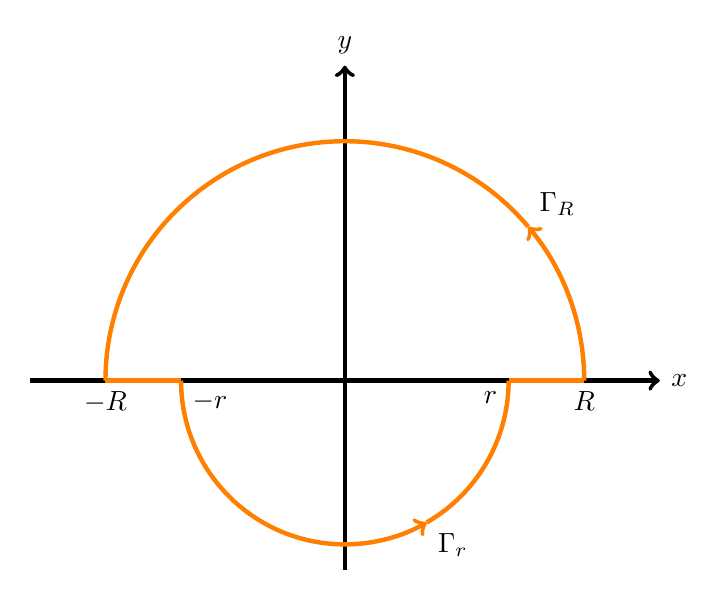
\begin{tikzpicture}[scale=.8]
		\draw[ultra thick,->]
			(-5,0)--(5,0)node[right]{\(x\)};
		\draw[ultra thick,->]
			(0,-3)--(0,5)node[above]{\(y\)};
		\pgfmathsetmacro{\R}{3.8}
		\pgfmathsetmacro{\r}{2.6}
		\begin{scope}[ultra thick,orange]
			\draw (-\R,0)node[below,black]{\(-R\)}--(-\r,0)node[below right,black]{\(-r\)} (\r,0)node[below left,black]{\(r\)}--(\R,0)node[below,black]{\(R\)};
			\draw[->] (-\r,0)arc[start angle=180,end angle=300,radius=\r]node[below right,black]{\(\Gamma_r\)};
			\draw (\r,0)arc[start angle=0,end angle=-60,radius=\r];
			\draw[->] (\R,0)arc[start angle=0,end angle=40,radius=\R]node[above right,black]{\(\Gamma_R\)};
			\draw (-\R,0)arc[start angle=180,end angle=40,radius=\R];
		\end{scope}
	\end{tikzpicture}
	\caption{狄利克雷积分的辅助积分路径}
	\label{figure:留数定理.狄利克雷积分的辅助积分路径}
\end{figure}

设\(f(z) = \frac{1}{z}\),
\(F(z) = \frac{e^{\iu z}}{z}\),
则\(F(z)\)中的\(z\)取实值\(x\)时,
其虚部即所求实积分的被积函数.
因为\(z=0\)是\(F(z)\)的一阶极点,
它处在\cref{theorem:留数定理.利用留数定理计算实积分3} 中
对辅助函数\(F(z) = e^{\iu\alpha z} f(z)\)的围线积分的积分路径上,
所以不能直接应用\cref{equation:留数定理.利用留数定理计算实积分3.1}.
我们改为考虑取\cref{figure:留数定理.狄利克雷积分的辅助积分路径} 所示的积分路径来绕开奇点,
再应用\hyperref[theorem:留数定理.柯西留数定理]{留数定理},
得\begin{align*}
	&\hspace{-20pt}\int_r^R F(x) \dd{x}
	+ \int_{\Gamma_R} F(z) \dd{z}
	+ \int_{-R}^{-r} F(x) \dd{x}
	+ \int_{\Gamma_r} F(z) \dd{z} \\
	&= 2\pi\iu \Res_{z=0} F(z)
	= 2\pi\iu \Res_{z=0} \frac{e^{\iu z}}{z}
	= 2\pi\iu,
\end{align*}
又由\hyperref[theorem:留数定理.计算积分路径上没有奇点的无穷限积分.引理2]{若尔当引理},
有\[
	\lim_{R\to+\infty} \int_{\Gamma_R} F(z) \dd{z} = 0.
\]
在\(\Gamma_r\)上的积分,
根据\(\lim_{z\to0} z F(z) = 1\),
以及\cref{theorem:留数定理.计算积分路径上没有奇点的无穷限积分.引理1},
有\[
	\lim_{r\to0} \int_{\Gamma_r} F(z) \dd{z} = \pi\iu.
\]
又因\[
	\int_{-R}^{-r} F(x) \dd{x}
	= \int_{-R}^{-r} \frac{e^{\iu x}}{x} \dd{x}
	= -\int_r^R \frac{e^{-\iu x}}{x} \dd{x},
\]
所以\[
	\int_r^R \frac{e^{\iu x} - e^{-\iu x}}{x} \dd{x}
	+ \int_{\Gamma_R} F(z) \dd{z}
	+ \int_{\Gamma_r} F(z) \dd{z}
	= 2\pi\iu,
\]
即\[
	2\iu \int_r^R \frac{\sin x}{x} \dd{x}
	+ \int_{\Gamma_R} F(z) \dd{z}
	+ \int_{\Gamma_r} F(z) \dd{z}
	= 2\pi\iu.
\]
令\(r\to0, R\to+\infty\),
即得\(\int_0^{+\infty} \frac{\sin x}{x} \dd{x} = \frac{\pi}{2}\).
\end{solution}
\end{example}

\subsection{其他情形}
还有一些无穷限积分,
不满足\cref{theorem:留数定理.利用留数定理计算实积分2,theorem:留数定理.利用留数定理计算实积分3} 的条件,
不能简单地引用这些定理来进行计算,
但我们可以借鉴这些定理的证明思路:
构造围线积分,
应用留数定理(或作为其特殊情形的柯西积分定理),
估计或计算辅助函数在辅助积分路径上的积分,
再取极限,
进而得到我们所要计算的广义积分.

\begin{example}
计算泊松积分\[
	I = \int_0^{+\infty} e^{-ax^2} \cos bx \dd{x} \quad(a>0).
\]
\begin{solution}
若\(b=0\),
则令\(t=\sqrt{a}x\)之后,
\[
	I = \int_0^{+\infty} e^{-ax^2} \dd{x}
	= \frac{1}{\sqrt{a}} \int_0^{+\infty} e^{-t^2} \dd{t}
	= \frac{1}{\sqrt{a}} \cdot \frac{\sqrt{\pi}}{2}
	= \frac{1}{2} \sqrt{\frac{\pi}{a}}.
	\eqno(1)
\]

若\(b\neq0\),
因为\(\cos bx\)是偶函数,
所以只需考虑\(b > 0\)的情形.
首先取辅助函数\(F_1(z) = e^{-az^2} e^{\iu bz}\),
则\begin{align*}
	I &= \frac{1}{2} \Re \int_{-\infty}^{+\infty} e^{-(ax^2+\iu bx)} \dd{x} \\
	&= \frac{1}{2} \Re\left\{
			e^{-\frac{b^2}{4a}}
			\int_{-\infty}^{+\infty}
			e^{-a\left(x+\frac{b}{2a}\iu\right)^2} \dd{x}
		\right\} \\
	&= \frac{1}{2} e^{-\frac{b^2}{4a}}
		\int_{-\infty+\frac{b}{2a}\iu}^{+\infty+\frac{b}{2a}\iu} e^{-az^2} \dd{z}.
	\tag2
\end{align*}

又由(1)式可知\[
	\int_{-\infty}^{+\infty} e^{-ax^2} \dd{x}
	= \sqrt{\frac{\pi}{a}}.
	\eqno(3)
\]

\begin{figure}[ht]
	\centering
	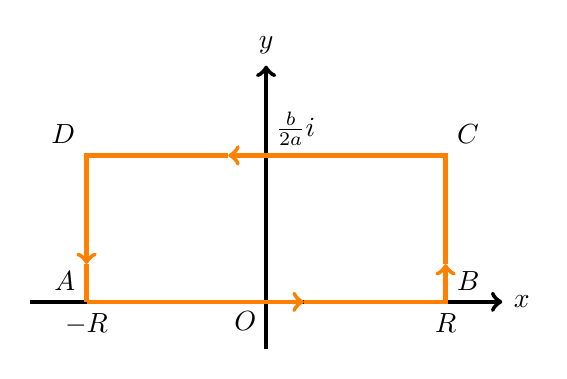
\begin{tikzpicture}[scale=.6]
		\draw[ultra thick,->]
			(-5,0)--(5,0)node[right]{\(x\)};
		\draw[ultra thick,->]
			(0,-1)--(0,5)node[above]{\(y\)};
		\pgfmathsetmacro{\R}{3.8}
		\pgfmathsetmacro{\b}{3.1}
		\begin{scope}[ultra thick,orange]
			\draw[->] (-\R,0)node[above left,black]{\(A\)}node[below,black]{\(-R\)}--(.8,0);
			\draw[->] (.8,0)--(\R,0)node[above right,black]{\(B\)}node[below,black]{\(R\)}--(\R,.8);
			\draw[->] (\R,.8)--(\R,\b)node[above right,black]{\(C\)}--(-.8,\b);
			\draw[->] (-.8,\b)--(-\R,\b)node[above left,black]{\(D\)}--(-\R,.8);
			\draw (-\R,.8)--(-\R,0);
		\end{scope}
		\draw (0,\b)node[above right]{\(\frac{b}{2a}i\)};
		\draw (0,0)node[below left]{\(O\)};
	\end{tikzpicture}
	\caption{泊松积分的辅助积分路径}
	\label{figure:留数定理.泊松积分的辅助积分路径}
\end{figure}
取辅助函数\(F(z) = e^{-az^2}\),
再取\cref{figure:留数定理.泊松积分的辅助积分路径} 所示的积分路径\(\Gamma = AB+BC+CD+DA\).
由\hyperref[theorem:解析函数的积分表示.柯西积分定理]{柯西积分定理}得\[
	\int_\Gamma e^{-az^2} \dd{z} = 0.
	\eqno(4)
\]

比较(2)式与(4)式,
得到\begin{align*}
	I &\xlongequal{\rm(2)}
		\frac{1}{2} e^{-\frac{b^2}{4a}}
		\Re\left[
			\lim_{R\to+\infty}
			\left( \int_{DC} e^{-az^2} \dd{z} \right)
		\right] \\
	&\xlongequal{\rm(4)}
		\frac{1}{2} e^{-\frac{b^2}{4a}}
		\Re\left[
			\lim_{R\to+\infty}
			\left( \int_{AB} + \int_{BC} + \int_{DA}\right)
			e^{-az^2} \dd{z}
		\right].
\end{align*}
在线段\(BC\)及\(DA\)上,
\(z=\pm R+\iu y\ (0 \leq y \leq \frac{b}{2a})\),
\[
	\abs{e^{-az^2}}
	= e^{-a(R^2-y^2)}
	\leq e^{\frac{b^2}{4a}} \cdot e^{-aR^2},
\]
故\[
	\lim_{R\to+\infty} \int_{BC} e^{-az^2} \dd{z} = 0,
	\qquad
	\lim_{R\to+\infty} \int_{DA} e^{-az^2} \dd{z} = 0.
\]
最后得到\[
	I = \frac{1}{2} e^{-\frac{b^2}{4a}} \Re\left[ \lim_{R\to+\infty} \int_{AB} e^{-az^2} \dd{z} \right]
	\xlongequal{\rm(3)} \frac{1}{2} \sqrt{\frac{\pi}{a}} e^{-\frac{b^2}{4a}},
\]
即\begin{equation}\label{equation:留数定理.泊松积分}
	\int_0^{+\infty} e^{-ax^2} \cos bx \dd{x}
	= \frac{1}{2} \sqrt{\frac{\pi}{a}} e^{-\frac{b^2}{4a}}
	\quad(a>0).
\end{equation}
\end{solution}
\end{example}

\begin{example}
计算菲涅耳积分\[
	\int_0^{+\infty} \cos x^2 \dd{x}
	\quad\text{及}\quad
	\int_0^{+\infty} \sin x^2 \dd{x}.
\]
\begin{solution}
\begin{figure}[ht]
	\centering
	\begin{tikzpicture}
		\draw[thick,->]
			(-.1,0)--(4.3,0)node[right]{\(x\)};
		\pgfmathsetmacro{\R}{4}
		\pgfmathsetmacro{\bx}{\R*cos(45)}
		\pgfmathsetmacro{\by}{\R*sin(45)}
		\coordinate (O) at (0,0);
		\coordinate (A) at (\R,0);
		\coordinate (B) at (\bx,\by);
		\draw pic["\(\frac{\pi}{4}\)",draw=blue,-,angle eccentricity=1.5,angle radius=8mm]{angle=A--O--B};
		\begin{scope}[ultra thick,orange]
			\draw[->] (O)--(3,0)node[below,black]{\(\Gamma_R\)};
			\draw (3,0)--(A)node[below,black]{\(R\)}arc[start angle=0,end angle=45,radius=\R]--(O);
		\end{scope}
		\draw (O)node[below left]{\(O\)};
	\end{tikzpicture}
	\caption{菲涅耳积分的辅助积分路径}
	\label{figure:留数定理.菲涅耳积分的辅助积分路径}
\end{figure}

选取辅助函数\(F(z) = e^{-z^2}\),
并取如\cref{figure:留数定理.菲涅耳积分的辅助积分路径} 所示的辅助积分路径\(C_R\),
则由柯西积分定理有\[
	\int_{C_R} e^{-z^2} \dd{z}
	= \int_0^R e^{-x^2} \dd{x}
	+ \int_{\Gamma_R} e^{-z^2} \dd{z}
	+ \int_R^0 \exp[-\left(x e^{\frac{1}{4}\pi\iu}\right)^2] \dd(x e^{\frac{1}{4}\pi\iu})
	= 0.
\]
在\(\Gamma_R\)上,
\(z = R e^{\iu\theta}\ (0\leq\theta\leq\frac{\pi}{4})\),
\(z^2 = R^2 e^{\iu2\theta}\).
利用\hyperref[equation:微分中值定理.若尔当不等式]{若尔当不等式}\[
	0\leq\theta\leq\frac{\pi}{2}
	\implies
	\sin\theta\geq\frac{2\theta}{\pi},
\]
可得\begin{align*}
	\abs{\int_{\Gamma_R} e^{-z^2} \dd{z}}
	&\leq
	\int_0^{\frac{\pi}{4}} \exp(-R^2 \cos2\theta) R\dd{\theta} \\
	&\xlongequal{2\theta=\frac{\pi}{2}-\phi}
	\frac{R}{2} \int_0^{\frac{\pi}{2}} \exp(-R^2 \sin\phi) \dd{\phi} \\
	&\leq
	\frac{R}{2} \int_0^{\frac{\pi}{2}} \exp(-\frac{2R^2}{\pi}\phi) \dd{\phi} \\
	&= \frac{\pi}{4R} (1-e^{-R^2})
	\to0\quad(R\to+\infty).
\end{align*}
所以\[
	\lim_{R\to+\infty} \left[
		\int_0^R \exp(-x^2) \dd{x}
		+ \int_R^0 \exp(-x^2 e^{\frac{1}{2}\pi\iu})
		\cdot \exp(\frac{1}{4}\pi\iu) \dd{x}
	\right] = 0,
\]\[
	\int_0^{+\infty} \exp(-x^2) \dd{x}
	- \exp(\frac{1}{4}\pi\iu)
	\int_0^{+\infty} (\cos x^2 - \iu \sin x^2) \dd{x} = 0.
\]
又因为\(\int_0^{+\infty} e^{-x^2} \dd{x} = \frac{\sqrt{\pi}}{2}\),
故\[
	\int_0^{+\infty} \cos x^2 \dd{x}
	- \iu \int_0^{+\infty} \sin x^2 \dd{x}
	= \frac{\sqrt{\pi}}{2} \exp(-\frac{1}{4}\pi\iu)
	= \frac{\sqrt{\pi}}{2} \left(\cos\frac{\pi}{4} - \iu \sin\frac{\pi}{4}\right).
\]
比较实部、虚部得\begin{equation}\label{equation:留数定理.菲涅耳积分}
	\int_0^{+\infty} \cos x^2 \dd{x}
	= \int_0^{+\infty} \sin x^2 \dd{x}
	= \frac{1}{2} \sqrt{\frac{\pi}{2}}.
\end{equation}
\end{solution}
\end{example}

从前面的几个模式可见,
利用留数定理计算实积分,
难点和关键在于选择恰当的辅助函数以及一条相应的辅助积分路径.
除了一些标准模式外,
辅助函数尤其是辅助积分路径的选择很不规则.
一般来说,辅助函数\(F(z)\)总要选得使\(z\)取实值\(x\)时,
\(F(x)\)等于实积分的被积函数\(f(x)\),
或\(\Re{F(z)} = f(x)\),
或\(\Im{F(z)} = f(x)\).
辅助积分路径的选择原则是:
使添加的积分路径上的复积分能够通过一定的办法估计或计算出来,
或者能够转化为原来要计算的实积分.
但具体选择时,形状则是多种多样的,
有半圆周围线、长方形围线、扇形围线、三角形围线等等.
此外,围线上有奇点时还要绕开奇点.

\subsection{计算多值函数的积分}
在计算某些广义实积分时,
需要选择的辅助函数有时是多值函数,
这时必须适当割破复平面,
使多值函数能够分出单值解析分支,
才能应用柯西留数定理或柯西积分定理,
进而求出所给广义实积分的值.

\subsubsection{计算\texorpdfstring{\(\int_0^{+\infty} f(x) \ln x \dd{x}\)型}{含有对数函数的}无穷限积分}
利用留数定理计算这种形式的积分时,
其辅助函数的选择就避不开多值函数\(\Ln z\).
为了使\(z\)取实值时\(\Ln z\)取实积分被积函数中的\(\ln x\),
我们必须割破\(z\)平面,
使\(\Ln z\)能够分出单值的解析分支,
并取其中的主值\(\ln z\).
在前面谈到将\(\Ln z\)分出单值解析分支时,
我们总是从原点起沿负实轴割破\(z\)平面.
其实从原点起沿正实轴割破\(z\)平面也能将\(\Ln z\)分出单值解析分支.
在下面的定理,限制\(0 < \Im \ln z = \arg z < 2\pi\),
也就意味着是沿正实轴割破\(z\)平面的.

\begin{theorem}\label{theorem:留数定理.利用留数定理计算实积分4}
若函数\(f(z)\)在扩充复平面\(\mathbb{C}_\infty\)上只有有限个孤立奇点\(\AutoTuple{a}{n}\),
且这些奇点不在包括原点的正实轴上,
\(f(z)\)在实轴上取实值,
此外\(z=\infty\)是\(f(z)\)的\(m\ (m\geq2)\)阶零点,
则\begin{equation}\label{equation:留数定理.利用留数定理计算实积分4.1}
	\int_0^{+\infty} f(x) \ln x \dd{x}
	= -\frac{1}{2} \Re{ \sum_{k=1}^n \Res_{z=a_k} \left[ f(z) \ln^2 z \right] },
\end{equation}
其中\(\ln z\)是复对数函数\(\Ln z\)的主值,
\(0<\Im \ln z<2\pi\).

特别地,若\(f(x) = \frac{P_n(x)}{Q_m(x)}\)是实系数的有理分式函数,
分母多像是\(Q_m(x)\)的零点不在包括原点的正实轴上,
且\(Q_m(x)\)的次数\(m\)至少比\(P_n(x)\)的次数\(n\)大\(2\),
即\(m-n\geq2\),
则\cref{equation:留数定理.利用留数定理计算实积分4.1} 成立.
\begin{proof}
\begin{figure}[ht]
	\centering
	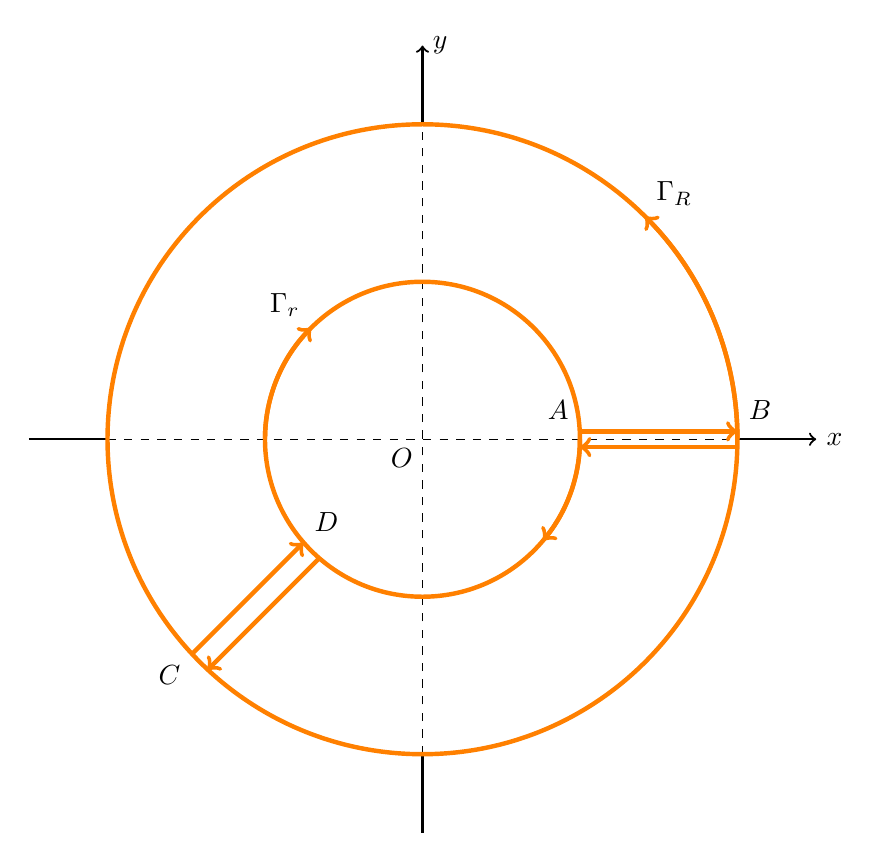
\begin{tikzpicture}
		\pgfmathsetmacro{\R}{4}
		\pgfmathsetmacro{\r}{2}
		\pgfmathsetmacro{\cx}{\R*cos(225)}
		\pgfmathsetmacro{\cy}{\R*sin(225)}
		\pgfmathsetmacro{\dx}{\r*cos(225)}
		\pgfmathsetmacro{\dy}{\r*sin(225)}
		\draw[thick,->]
			(-5,0)--(-\R,0) (\R,0)--(5,0)node[right]{\(x\)};
		\draw[thick,->]
			(0,-5)--(0,-\R) (0,\R)--(0,5)node[right]{\(y\)};
		\draw[dashed] (-\R,0)--(\R,0) (0,-\R)--(0,\R);
		\coordinate (O) at (0,0);
		\coordinate (A) at (\r,.1);
		\coordinate (B) at (\R,.1);
		\begin{scope}[ultra thick,orange]
			\draw (O)circle(\R)circle(\r);
			\begin{scope}[->]
				\draw (A)node[above left,black]{\(A\)}--(B)node[above right,black]{\(B\)};
				\draw (\R,-.1)--(\r,-.1);
				\draw (\R,0)arc[start angle=0,end angle=45,radius=\R]node[above right,black]{\(\Gamma_R\)};
				\draw (-\r,0)arc[start angle=180,end angle=135,radius=\r]node[above left,black]{\(\Gamma_r\)};
				\draw (\r,0)arc[start angle=0,end angle=-40,radius=\r];
				\draw (\cx-.1,\cy+.1)node[below left,black]{\(C\)}--(\dx-.1,\dy+.1)node[above right,black]{\(D\)};
				\draw (\dx+.1,\dy-.1)--(\cx+.1,\cy-.1);
			\end{scope}
		\end{scope}
		\draw (O)node[below left]{\(O\)};
	\end{tikzpicture}
	\caption{}
	\label{figure:留数定理.利用留数定理计算实积分4的辅助积分路径1}
\end{figure}
取辅助围线如\cref{figure:留数定理.利用留数定理计算实积分4的辅助积分路径1} 所示的\[
	\Gamma = AB \cup \Gamma_R \cup BA \cup \Gamma_r^-,
\]
其中\(AB\)沿支割线上岸,
\(BA\)沿支割线下岸\footnote{曲线\(\Gamma\)虽不是简单闭曲线,
但用连接内外圆周的直线段\(CD\)可将\(\Gamma\)变为两条简单闭曲线,
在它们所围的两个区域内应用留数定理,
由于在线段\(CD\)上来回积分两次,
其和为零,
所以可在\(\Gamma\)所围区域内应用留数定理.}.
取辅助函数\[
	F(z) = f(z) \ln^2 z,
\]
其中\(\ln z\)是\(\Ln z\)的主值,
而\(0<\Im\ln z<2\pi\).
\(F(z)\)在\(\Gamma\)的“内部”(除\(\AutoTuple{a}{n}\))解析,
且连续到边界\(\Gamma\)(在\(AB,BA\)上分别是从上、下半平面连续到\(AB,BA\)).
由留数定理,
得\[
	\left(\int_{AB}+\int_{\Gamma_R}+\int_{BA}+\int_{\Gamma_r^-}\right) F(z) \dd{z}
	= 2\pi\iu \sum_{k=1}^n \Res_{z=a_k} F(z).
\]

在线段\(AB\)上,\(z=x\),\(F(z) = f(x) \ln^2 x\),
因此\[
	\int_{AB} F(z) \dd{z}
	= \int_r^R f(x) \ln^2 x \dd{x}.
\]

在线段\(BA\)上,\(z = x e^{2\pi\iu}\),\(F(z) = f(x) (\ln x + 2\pi\iu)^2\),
所以\[
	\int_{BA} F(z) \dd{z}
	= -\int_r^R f(x) (\ln x + 2\pi\iu)^2 \dd{x}.
\]

在\(\Gamma_R\)上,\(z = R e^{\iu\theta}\ (0\leq\theta\leq2\pi)\),\[
	\abs{\ln z}^2 = \ln^2 R + \theta^2 \leq 2 \ln^2 R.
\]

点\(z=\infty\)是\(f(z)\)的\(m\)阶零点.
当\(R\)充分大时,\(\abs{f(z)} \leq M/R^m\ (M>0)\).
于是,\[
	\abs{\int_{\Gamma_R} F(z) \dd{z}}
	\leq \frac{M}{R^m} \cdot 2 \ln^2 R \cdot 2\pi R
	= \frac{4M \ln^2 R}{R^{m-1}} \to 0 \quad(R\to+\infty).
\]

在\(\Gamma_r\)上,\(z = r e^{\iu\theta}\ (0\leq\theta\leq2\pi)\),
从而\[
	\abs{\ln z}^2 = \ln^2 r + \theta^2
	\leq 2 \ln^2 \frac{1}{r}.
\]

\(f(z)\)在点\(z=0\)的邻域内有界,
所以\[
	\abs{F(z)} \leq 2M_1 \ln^2 \frac{1}{r},
\]\[
	\abs{\int_{\Gamma_r} F(z) \dd{z}}
	\leq 4\pi M_1 r \ln^2 \frac{1}{r}
	\to 0 \quad(r\to0^+).
\]

于是,\(r\to0^+, R\to+\infty\)时,
有\[
	\int_0^{+\infty} f(x) \ln^2 x \dd{x}
	- \int_0^{+\infty} f(x) (\ln x + 2\pi\iu)^2 \dd{x}
	= 2\pi\iu \sum_{k=1}^n \Res_{z=a_k} F(z),
\]\[
	-4\pi\iu \int_0^{+\infty} f(x) \ln x \dd{x}
	+ 4\pi^2 \int_0^{+\infty} f(x) \dd{x}
	= 2\pi\iu \sum_{k=1}^n \Res_{z=a_k} F(z).
\]
在上式两边取虚部,
即得\begin{equation}\label{equation:留数定理.利用留数定理计算实积分4.2}
	\int_0^{+\infty} f(x) \ln x \dd{x}
	= -\frac{1}{2} \Re{ \sum_{k=1}^n \Res_{z=a_k} \left[ f(z) \ln^2 z \right] };
\end{equation}
取实部,
即得\begin{equation}\label{equation:留数定理.利用留数定理计算实积分4.3}
	\int_0^{+\infty} f(x) \dd{x}
	= -\frac{1}{2\pi} \Im{ \sum_{k=1}^n \Res_{z=a_k} \left[ f(z) \ln^2 z \right] }.
\end{equation}
\end{proof}
\end{theorem}

\begin{figure}[ht]
	\centering
	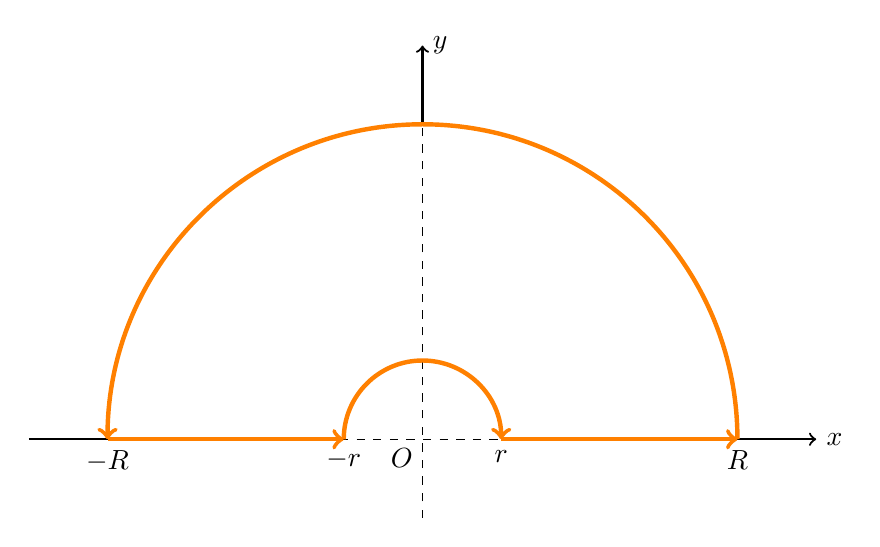
\begin{tikzpicture}
		\pgfmathsetmacro{\R}{4}
		\pgfmathsetmacro{\r}{1}
		\draw[thick,->]
			(-5,0)--(-\R,0) (\R,0)--(5,0)node[right]{\(x\)};
		\draw[thick,->]
			(0,\R)--(0,5)node[right]{\(y\)};
		\draw[dashed] (-\R,0)--(\R,0) (0,-1)--(0,\R);
		\coordinate (O) at (0,0);
		\begin{scope}[ultra thick,orange]
			\begin{scope}[->]
				\draw (\r,0)node[below,black]{\(r\)}--(\R,0)node[below,black]{\(R\)};
				\draw (\R,0)arc[start angle=0,end angle=180,radius=\R];
				\draw (-\R,0)node[below,black]{\(-R\)}--(-\r,0)node[below,black]{\(-r\)};
				\draw (-\r,0)arc[start angle=180,end angle=0,radius=\r];
			\end{scope}
		\end{scope}
		\draw (O)node[below left]{\(O\)};
	\end{tikzpicture}
	\caption{}
	\label{figure:留数定理.利用留数定理计算实积分4的辅助积分路径2}
\end{figure}
若\(f(x)\)是偶函数,
\(f(z)\)在上半平面\(\Im z > 0\)内
除去有限多个孤立奇点\(\AutoTuple{a}{n}\)外是解析的,
在\(\Im z \geq 0\)上除去\(\AutoTuple{a}{n}\)外连续,
且\[
	(\exists M>0)
	(\forall m\geq2)
	(\exists N>0)
	[
		\abs{z}>N
		\implies
		\abs{f(z)}\leq\frac{M}{\abs{z}^m}
	]
\]
则令\(F(z) = f(z) \ln z\),
并取如\cref{figure:留数定理.利用留数定理计算实积分4的辅助积分路径2} 所示的辅助围线,
则有\begin{gather}
	\int_0^{+\infty} f(x) \ln x \dd{x}
		= -\pi \Im{ \sum_{k=1}^n \Res_{z=a_k}[ f(z) \ln z ] },
		\label{equation:留数定理.利用留数定理计算实积分4.4} \\
	\int_0^{+\infty} f(x) \dd{x}
		= 2 \Re{ \sum_{k=1}^n \Res_{z=a_k}[ f(z) \ln z ] }.
		\label{equation:留数定理.利用留数定理计算实积分4.5}
\end{gather}

\begin{example}
计算积分\[
	I = \int_0^{+\infty} \frac{\ln x}{(1+x^2)^2} \dd{x}.
\]
\begin{solution}
因为函数\(f(x) = \frac{1}{(1+x^2)^2}\)是偶函数,
也可用\cref{equation:留数定理.利用留数定理计算实积分4.4}
计算这个积分:\begin{align*}
	\Res_{z=\iu} \frac{\ln z}{(1+z^2)^2}
	&= \eval{\left\{ \dv{z} \left[ \frac{\ln z}{(z+\iu)^2} \right] \right\}}_{z=\iu} \\
	&= \eval{\left\{ \frac{1}{z(z+\iu)^2} - \frac{2 \ln z}{(z+\iu)^3} \right\}}_{z=\iu} \\
	&= \frac{\pi}{8} + \frac{\iu}{4},
\end{align*}\[
	\int_0^{+\infty} \frac{\ln x}{(1+x^2)^2} \dd{z}
	= -\pi \Im\left(\frac{\pi}{8}+\frac{\iu}{4}\right)
	= -\frac{\pi}{4}.
\]
\end{solution}
\end{example}

\subsubsection{计算\texorpdfstring{\(\int_0^{+\infty} f(x) x^{p-1} \dd{x}\ (0<p<1)\)型}{含有幂函数的}无穷限积分}
\begin{theorem}\label{theorem:留数定理.利用留数定理计算实积分5}
若函数\(f(z)\)在扩充复平面\(\mathbb{C}_\infty\)上
除去有限个点\(\AutoTuple{a}{n}\)外解析,
且\(\AutoTuple{a}{n}\)不在包括原点的正实轴上,
点\(z=\infty\)是\(f(z)\)的\(m\ (m\geq1)\)阶零点,
则\begin{equation}\label{equation:留数定理.利用留数定理计算实积分5.1}
	\int_0^{+\infty} f(x) x^{p-1} \dd{x}
	= \frac{2\pi\iu}{1-e^{2\pi p\iu}} \sum_{k=1}^n \Res_{z=a_k}[f(z) z^{p-1}],
\end{equation}
其中\(z^{p-1} = e^{(p-1) \ln z}\ (0<\Im\ln z = \arg z<2\pi)\).

特别地,若\(f(x) = \frac{P_n(x)}{Q_m(x)}\)是有理分式函数,
\(Q_m(x)\)在包括原点的正实轴上没有零点,
分母多项式\(Q_m(x)\)的次数\(m\)比分子多项式\(P_n(x)\)的次数\(n\)至少大\(1\),
即\(m-n\geq1\),
则\cref{equation:留数定理.利用留数定理计算实积分5.1} 成立.
\begin{proof}
取辅助函数\(F(z) = z^{p-1} f(z) = e^{(p-1)\ln z} f(z)\),
其中\[
	\ln z = \ln\abs{z} + \iu\arg z \quad(0<\arg z<2\pi).
\]
取辅助围线\(C\)如\cref{figure:留数定理.利用留数定理计算实积分4的辅助积分路径1} 所示,
\(C=AB+\Gamma_R+BA+\Gamma_r^-\).
由留数定理,
得\begin{align*}
	&\hspace{-20pt}\int_r^R e^{(p-1)\ln x} f(x) \dd{x}
		+ \int_{\Gamma_R} F(z) \dd{z}
		+ \int_R^r e^{(p-1)(\ln x+2\pi\iu)} f(x) \dd{x}
		+ \int_{\Gamma_r^-} F(z) \dd{z} \\
	&= 2\pi\iu \sum_{k=1}^n \Res_{z=a_k} F(z),
\end{align*}
整理得\[
	(1-e^{2\pi p\iu}) \int_r^R x^{p-1} f(x) \dd{x}
	+ \left(\int_{\Gamma_r^-}+\int_{\Gamma_R}\right) F(z) \dd{z}
	= 2\pi\iu \sum_{k=1}^n \Res_{z=a_k} F(z).
	\eqno(1)
\]

在\(\Gamma_r\)上有\begin{align*}
	\abs{\int_{\Gamma_r^-} F(z) \dd{z}}
	&= \abs{\int_{\Gamma_r^-} e^{(p-1)(\ln r + \iu\arg z)} f(z) \dd{z}} \\
	&= r^{p-1} \max_{z\in\Gamma_r} \abs{f(z)} \cdot 2\pi r \\
	&= 2\pi r^p \max_{z\in\Gamma_r} \abs{f(z)} \to0\quad(r\to0),
\end{align*}
同理有\[
	\abs{\int_{\Gamma_R} F(z) \dd{z}}
	\leq 2\pi R^p \max_{z\in\Gamma_R} \abs{f(z)}.
\]

由于\(z=\infty\)为\(f(z)\)的\(m\)阶零点,
当\(R\)充分大时,
在\(\Gamma_R\)上\(\abs{f(z)}<M/R^m\),
\(M\)是正常数,
\(m\geq1\),
所以\[
	\abs{\int_{\Gamma_R} F(z) \dd{z}}
	\leq \frac{2\pi M}{R^{m-p}} \to0\quad(R\to+\infty).
\]
在(1)式中令\(r\to0^+,R\to+\infty\),
得到\[
	(1-e^{2\pi p\iu}) \int_0^{+\infty} x^{p-1} f(x) \dd{x}
	= 2\pi\iu \sum_{k=1}^n \Res_{z=a_k} F(z).
\]
于是得到\cref{equation:留数定理.利用留数定理计算实积分5.1}
或者\begin{equation}\label{equation:留数定理.利用留数定理计算实积分5.2}
	\int_0^{+\infty} x^{p-1} f(x) \dd{x}
	= -\frac{\pi}{e^{p\pi\iu} \sin p\pi} \sum_{k=1}^n \Res_{z=a_k}[z^{p-1} f(z)].
\end{equation}
注:关于\(p\),只要假定\(0<p<m\),
且\(p\notin\mathbb{Z}\),
则\cref{equation:留数定理.利用留数定理计算实积分5.1} 成立.
若\(f(x)\)是偶函数,
仍可采用\cref{figure:留数定理.利用留数定理计算实积分4的辅助积分路径2} 所示的积分路径,
得出相应的结果.
\end{proof}
\end{theorem}

\begin{example}
计算欧拉积分\[
	I = \int_0^{+\infty} \frac{x^{p-1}}{1+x} \dd{x} \quad(0<p<1).
\]
\begin{solution}
这里\(f(x) = \frac{1}{1+x}\)满足\cref{theorem:留数定理.利用留数定理计算实积分5} 的条件.
点\(z=-1\)是\(f(z) = \frac{1}{1+z}\)的一阶极点,
\(z=\infty\)是\(f(z)\)的一阶零点.
\(F(z) = z^{p-1} \frac{1}{1+z}\)在点\(z=-1\)处的留数\[
	\Res_{z=-1} F(z)
	= \lim_{z\to-1} (z+1) \frac{z^{p-1}}{1+z}
	= \lim_{\substack{\abs{z}\to1 \\ \theta\to\pi}} \exp[(p-1)(\ln\abs{z}+\iu\theta)]
	= e^{(p-1)\pi\iu}
	= -e^{p\pi\iu}.
\]
应用\cref{equation:留数定理.利用留数定理计算实积分5.2}
即有\begin{equation}
	\int_0^{+\infty} \frac{x^{p-1}}{1+x} \dd{x} = \frac{\pi}{\sin p\pi}.
\end{equation}
\end{solution}
\end{example}

\begin{example}%https://www.bilibili.com/video/BV1Vb4y1Y7Sn/
计算定积分\[
	\int_0^1 \frac{\ln x}{x^2-x-1} \dd{x}.
\]
\begin{solution}
首先求出所求积分\(I = \int_0^1 \frac{\ln x}{x^2-x-1} \dd{x}\)的奇点,
即方程\(x^2-x-1=0\)的根,
得\[
	x_1 = \frac{1-\sqrt{5}}{2}, \qquad
	x_2 = \frac{1+\sqrt{5}}{2}.
\]

取割线\(L = \Set{x \given x\in[0,1]} \cup \Set{1+\iu y \given y\in[0,+\infty)}\).
我们利用复对数函数\(\Ln z\)作为辅助函数,
并令\(\Ln\frac{1}{2} = \ln\frac{1}{2}\).
以\(L_1,L_2\)分别表示射线\(\Set{1+\iu y \given y\in[0,+\infty)}\)的右侧和左侧,方向向上;
以\(L_3,L_4\)分别表示线段\(\Set{x \given x\in[0,1]}\)的上侧和下侧,方向向右.

根据留数定理\[
	\left(\int_{L_2} - \int_{L_1} - \int_{L_4} + \int_{L_3}\right) \frac{\Ln^2 z}{z^2-z-1} \dd{z}
	= 2\pi\iu \left[\Res_{z=x_1} f(z) + \Res_{z=x_2} f(z)\right].
	\eqno(1)
\]

在\(L_2\)上,\(z=1+\iu y\),从而\(\abs{z}=\sqrt{1+y^2},
\arg z = \arctan y,
\dd{z} = \iu \dd{y}\),
\[
	\int_{L_2} \frac{\Ln^2 z}{z^2-z-1} \dd{z}
	= \int_0^{+\infty} \frac{\left(\ln\sqrt{1+x^2} + \iu \arctan x\right)^2}{-x^2+\iu x-1} \iu \dd{x}.
\]

在\(L_1\)上,因为它是下沿,所以\[
	\Ln^2 z = \left(\ln\sqrt{1+x^2} + \iu \arctan x + 2\pi\iu\right)^2,
\]
那么\[
	\int_{L_1} \frac{\Ln^2 z}{z^2-z-1} \dd{z}
	= \int_0^{+\infty} \frac{\left(
		\ln\sqrt{1+x^2}
			+ \iu \arctan x + 2\pi\iu
		\right)^2}{-x^2+\iu x-1}
		\iu \dd{x}.
\]

在\(L_4\)上,\(z=x\),
因为它是下沿,
所以\[
	\int_{L_4} \frac{\Ln^2 z}{z^2-z-1} \dd{z}
	= \int_0^1 \frac{\left(\ln x + 2\pi\iu\right)^2}{x^2-x-1} \dd{x}.
\]

在\(L_3\)上,\(z=x\),\[
	\int_{L_3} \frac{\Ln^2 z}{z^2-z-1} \dd{z}
	= \int_0^1 \frac{\ln^2 x}{x^2-x-1} \dd{x}.
\]

因为\[
	\Res_{z=x_1} f(z)
	= \frac{\left(\ln\abs{x_1} + \pi\iu\right)^2}{x_1 - x_2},
	\qquad
	\Res_{z=x_2} f(z)
	= \frac{\left(\ln\abs{x_2} + 2\pi\iu\right)^2}{x_2 - x_1},
\]
且(1)式左侧可化简得\begin{align*}
	2\pi \left(
		\int_0^{+\infty} \frac{2\ln\sqrt{1+x^2} + 2\iu \arctan x + 2\pi\iu}{-x^2+\iu x-1} \dd{x}
		+ \int_0^1 \frac{-2\iu \ln x + 2\pi}{x^2-x-1} \dd{x}
	\right),
\end{align*}
那么对(1)式两边取虚部并同除以\((-2\pi)\)可得\[
	-\Im \int_0^{+\infty} \frac{2\ln\sqrt{1+x^2} + 2\iu \arctan x + 2\pi\iu}{-x^2+\iu x-1} \dd{x}
	+ 2I = \frac{3\pi^2}{\sqrt{5}}.
\]

进行分母有理化,
有\begin{align*}
	&-\Im \int_0^{+\infty} \frac{2\ln\sqrt{1+x^2} + 2\iu \arctan x + 2\pi\iu}{-x^2+\iu x-1} \dd{x} \\
	&= -\Im \int_0^{+\infty} \frac{\left(2\ln\sqrt{1+x^2} + 2\iu \arctan x + 2\pi\iu\right) \left(-x^2-\iu x-1\right)}{(x^2+1)^2+x^2} \dd{x} \\
	&= \int_0^{+\infty} \frac{x \ln(1+x^2) + 2(\arctan x + \pi) (x^2+1)}{(x^2+1)^2+x^2} \dd{x} \\
	&= \int_0^{+\infty} \left[
	\frac{x \ln(1+x^2)}{(x^2+1)^2+x^2}
	+ 2\pi \cdot \frac{x^2+1}{(x^2+1)^2+x^2}
	+ 2 \cdot \frac{(x^2+1) \arctan x}{(x^2+1)^2+x^2}
	\right] \dd{x}.
\end{align*}

注意到\begin{align*}
	\int_0^{+\infty} \frac{x \ln(1+x^2)}{(x^2+1)^2+x^2} \dd{x}
	&= \frac{1}{2} \int_0^{+\infty} \frac{\ln(1+x)}{(x+1)^2+x} \dd{x} \\
	&= \frac{1}{2} \int_1^{+\infty} \frac{\ln x}{x^2+x-1} \dd{x}
	= \frac{I}{2},
\end{align*}
\begin{align*}
	\int_0^{+\infty} \frac{x^2+1}{(x^2+1)^2+x^2} \dd{x}
	&= \int_0^{+\infty} \frac{1}{\left(x-1/x\right)^2+5} \left(1+\frac{1}{x^2}\right) \dd{x} \\
	&= \int_{-\infty}^{+\infty} \frac{1}{u^2+5} \dd{u}
	= \frac{\pi}{\sqrt{5}},
\end{align*}
\begin{align*}
	\int_0^{+\infty} \frac{(x^2+1) \arctan x}{(x^2+1)^2+x^2} \dd{x}
	&= \int_0^{+\infty} \frac{(x^2+1) \arctan(1/x)}{(x^2+1)^2+x^2} \dd{x} \\
	&= \int_0^{+\infty} \frac{(x^2+1) (\pi/2 - \arctan x)}{(x^2+1)^2+x^2} \dd{x} \\
	&= \frac{\pi}{4} \int_0^{+\infty} \frac{x^2+1}{(x^2+1)^2+x^2} \dd{x}
	= \frac{\pi^2}{4\sqrt{5}},
\end{align*}
综上所述,\(\frac{I}{2} + \frac{2\pi^2}{\sqrt{5}} + \frac{\pi^2}{2\sqrt{5}} + 2I
= \frac{3\pi^2}{\sqrt{5}}\),
解得\[
	I = \int_0^1 \frac{\ln x}{x^2-x-1} \dd{x}
	= \frac{\pi^2}{5\sqrt{5}}.
\]
\end{solution}
\end{example}

\section{辐角原理及其应用}
这一节讨论在留数理论基础上建立起来的辐角原理,利用它可以解决一些解析函数的零点个数及分布问题.

\subsection{零点与极点个数定理}
\begin{lemma}
设\(a,b\)分别是函数\(f(z)\)的\(n\)阶零点和\(m\)阶极点,
则\(a,b\)都是函数\(\frac{f'(z)}{f(z)}\)的一阶极点,
且\[
	\Res_{z=a} \frac{f'(z)}{f(z)} = n,
	\qquad
	\Res_{z=b} \frac{f'(z)}{f(z)} = -m.
\]
\begin{proof}
设\(a\)是\(f(z)\)的\(n\)阶零点,
则在点\(a\)的邻域\(U(a)\)内有\[
	f(z) = (z-a)^n g(z),
\]
其中\(g(z)\)在\(N(a)\)内解析,且\(g(z)\neq0\).
于是\begin{align*}
	f'(z) &= n(z-a)^{n-1} g(z) + (z-a)^n g'(z), \\
	\frac{f'(z)}{f(z)} &= \frac{n}{z-a} + \frac{g'(z)}{g(z)}.
\end{align*}
由于\(\frac{g'(z)}{g(z)}\)在点\(a\)的邻域\(N(a)\)内解析,
故由上式得出\(a\)必是\(\frac{f'(z)}{f(z)}\)的一阶极点,
且\(\Res_{z=a} \frac{f'(z)}{f(z)} = n\).

若\(b\)是\(f(z)\)的\(m\)阶极点,
则在点\(b\)的去心邻域\(\mathring{U}(b)\)内有\[
	f(z) = \frac{h(z)}{(z-b)^m},
\]
其中\(h(z)\)在点\(b\)的邻域\(U(b)\)内解析,
且\(h(b)\neq0\).
由此易得\[
	\frac{f'(z)}{f(z)}
	= \frac{-m}{z-b} + \frac{h'(z)}{h(z)},
\]
而\(\frac{h'(z)}{h(z)}\)在点\(b\)的邻域\(U(b)\)内解析.
故\(b\)必是\(\frac{f'(z)}{f(z)}\)的一阶极点,
且\[
	\Res_{z=b} \frac{f'(z)}{f(z)} = -m.
	\qedhere
\]
\end{proof}
\end{lemma}

\begin{theorem}\label{theorem:留数定理.零点与极点个数定理}%定理5.3.1
设函数\(f(z)\)在围线\(C\)上解析且不为零,
在\(C\)的内部除可能有极点外是解析的,
则\begin{equation}\label{equation:留数定理.零点与极点个数定理1}
	\frac{1}{2\pi\iu}
	\int_C \frac{f'(z)}{f(z)} \dd{z}
	= N(f,C) - P(f,C),
\end{equation}
其中\(N(f,C)\)与\(P(f,C)\)分别表示
\(f(z)\)在\(C\)内部的零点与极点的个数
(一个\(n\)阶零点算作\(n\)个零点,而一个\(m\)阶极点算作\(m\)个极点).
\end{theorem}
\cref{theorem:留数定理.零点与极点个数定理} 被称为{解析函数的零点与极点个数定理}.

\begin{example}
计算积分\[
	I = \int_{\abs{z}=4} \frac{z^9}{z^{10}-1} \dd{z}.
\]
\begin{solution}
设\(f(z) = z^{10}-1\),
则\(f(z)\)在\(C: \abs{z}=4\)上解析且不等于零;
又因\(f(z)\)在\(\abs{z}<4\)内解析,
且有10个零点、0个极点,
即\[
	N(f,C) = 10, \qquad P(f,C) = 0.
\]
所以\begin{align*}
	I &= \frac{1}{10} \int_{\abs{z}=4} \frac{z^9}{z^{10}-1} \dd{z}
	= \frac{1}{10} \int_{\abs{z}=4} \frac{(z^{10}-1)'}{z^{10}-1} \dd{z} \\
	&= \frac{1}{10} \cdot 2\pi\iu (10-0) = 2\pi\iu.
\end{align*}
\end{solution}
\end{example}

\subsection{辐角原理及其应用}
\cref{theorem:留数定理.零点与极点个数定理} 的几何解释就称为辐角原理.
当变换\(w = f(z)\)满足\cref{theorem:留数定理.零点与极点个数定理} 的条件时,
它把\(z\)平面上围线\(C: z = z(t)\ (\alpha \leq t \leq \beta)\)
变成\(w\)平面上有向闭曲线\(\Gamma: w = f[z(t)]\ (\alpha \leq t \leq \beta)\).
由于\(z \in C\)时,
\(f(z)\neq0\),
所以\(w\)平面上曲线\(\Gamma\)不过原点.
于是\begin{equation}\label{equation:留数定理.辐角原理及其应用1}
	\frac{1}{2\pi\iu} \int_C \frac{f'(z)}{f(z)} \dd{z}
	= \frac{1}{2\pi\iu} \int_\Gamma \frac{\dd{w}}{w}.
\end{equation}

需要注意的是,虽然原象曲线\(C\)是简单闭曲线,
但其象曲线\(\Gamma\)只能肯定是有向闭曲线,
\(\Gamma\)未必是简单闭曲线.
当\(\Gamma\)是简单闭曲线时,
在\(\Gamma\)内部含有原点的情况下,
我们知道\cref{equation:留数定理.辐角原理及其应用1} 右端积分为\(1\);
在\(\Gamma\)内部不含原点的情况下,
\cref{equation:留数定理.辐角原理及其应用1} 右端积分为\(0\).
当\(\Gamma\)是一般的不过原点有向闭曲线时,
由\[
	\frac{1}{2\pi\iu} \int_\Gamma \frac{\dd{w}}{w}
	= \frac{1}{2\pi\iu} \int_\Gamma \dd(\ln w)
	= \frac{1}{2\pi\iu} \left[ \int_\Gamma \dd(\ln\abs{w}) + \iu \int_\Gamma \dd(\arg w) \right],
\]
函数\(\ln\abs{w}\)是\(w\)的单值函数.
\(w\)从\(w_0\)起沿\(\Gamma\)连续变动回到\(w_0\)时\[
	\int_\Gamma \dd(\ln\abs{w})
	= \ln\abs{w_0} - \ln\abs{w_0} = 0,
\]
得到\begin{equation}\label{equation:留数定理.辐角原理及其应用2}
	\frac{1}{2\pi\iu} \int_\Gamma \frac{\dd{w}}{w}
	= \frac{1}{2\pi} \int_\Gamma \dd(\arg w).
\end{equation}
上式右端是\(w\)沿\(\Gamma\)连续变化回到出发点时它的辐角增量除以\(2\pi\),
也就是说,上式左端\(\frac{1}{2\pi\iu} \int_\Gamma \frac{\dd{w}}{w}\)
等于\(\Gamma\)绕原点的圈数(或称为\(\Gamma\)关于原点的环绕次数).
因为\(\Gamma\)是闭曲线,故这个“圈数”总是整数.
\begin{equation}\label{equation:留数定理.辐角原理及其应用3}
	\frac{1}{2\pi} \int_\Gamma \dd(\arg w)
	= \frac{1}{2\pi} \increment_\Gamma \arg w
	= \frac{1}{2\pi} \increment_C \arg f(z).
\end{equation}
综合\cref{equation:留数定理.零点与极点个数定理1,equation:留数定理.辐角原理及其应用1,equation:留数定理.辐角原理及其应用2,equation:留数定理.辐角原理及其应用3},
得到\begin{equation}\label{equation:留数定理.辐角原理及其应用4}
	N(f,C)-P(f,C) = \frac{1}{2\pi} \increment_C \arg f(z).
\end{equation}

这样,\cref{theorem:留数定理.零点与极点个数定理} 的几何解释就是:
在\cref{theorem:留数定理.零点与极点个数定理} 的条件下,
函数\(f(z)\)在围线\(C\)内部的零点个数与极点个数之差,
等于当\(z\)沿\(C\)的正向绕行一周后\(f(z)\)的辐角改变量\(\increment_C \arg f(z)\)除以\(2\pi\),
或者说,等于象曲线关于象平面原点的环绕次数,
即\cref{equation:留数定理.辐角原理及其应用4} 成立.

特别地,若\(f(z)\)在围线\(C\)上及\(C\)之内部解析,
且\(f(z)\)在\(C\)上不为零,
则\begin{equation}\label{equation:留数定理.辐角原理及其应用5}
	N(f,C) = \frac{1}{2\pi} \increment_C \arg f(z).
\end{equation}

\begin{example}
函数\[
	f(z) = \frac{(z^2+1)(z-4)}{\sin^4 z}
\]
在圆周\(C: \abs{z}=3\)的内部有两个1阶零点\(z=\pm\iu\)和一个4阶极点\(z=0\),
故\[
	N=N(f,C)=2, \qquad P=P(f,C)=4,
\]
所以\[
	\increment_C \arg f(z) = 2\pi(N - P) = -4\pi.
\]
也就是说,当动点\(z\)沿\(\abs{z}=3\)的正向绕行一周后,
\(w = f(z)\)的辐角增量为\(-4\pi\).
或者说,\(z\)平面上动点\(z\)沿圆周\(\abs{z}=3\)的正向行进一周时,
\(w\)平面上象点\(w\)将围绕原点\(w=0\)按顺时针方向绕行两周.
\end{example}

\begin{theorem}[儒歇定理]
设函数\(f(z)\)及\(g(z)\)在围线\(C\)及其内部解析,
且在\(C\)上有不等式\(\abs{f(z)}>\abs{g(z)}\)成立,
则在\(C\)内部\(f(z)+g(z)\)与\(f(z)\)的零点个数相等,
即\[
	N(f+g,C) = N(f,C).
\]
\begin{proof}
由于在\(C\)上有\(\abs{f(z)}>\abs{g(z)}\geq0\),从而\[
\abs{f(z)+g(z)}\geq\abs{f(z)}-\abs{g(z)}>0,
\]故\(f(z)\)及\(f(z)+g(z)\)在\(C\)上均无零点;
又因\(f(z)\)及\(f(z)+g(z)\)均在围线\(C\)及其内部解析,
从而它们都满足\cref{theorem:留数定理.零点与极点个数定理} 的条件.
于是由\cref{equation:留数定理.辐角原理及其应用5},
下面只需证明\begin{equation}\label{equation:留数定理.辐角原理及其应用6}
	\increment_C \arg[f(z)+g(z)] = \increment_C \arg f(z).
\end{equation}
由于\[
	f(z)+g(z) = f(z) \left[1+\frac{g(z)}{f(z)}\right],
\]
则有\begin{equation}\label{equation:留数定理.辐角原理及其应用7}
	\increment_C \arg[f(z)+g(z)]
	= \increment_C \arg f(z)
	+ \increment_C \arg\left[1+\frac{g(z)}{f(z)}\right].
\end{equation}
因在\(C\)上\(\abs{f(z)}>\abs{g(z)}\),
当\(z\)沿\(C\)变动时\(\abs{\frac{g(z)}{f(z)}}<1\).
经变换\(\eta=1+\frac{g(z)}{f(z)}\)
将\(z\)平面上的围线\(C\)
变成\(\eta\)平面上的闭曲线\(\Gamma\)之后,
\(\Gamma\)将全含于圆周\(\abs{\eta-1}=1\)的内部.
注意到原点\(\eta=0\)并不在圆周\(\abs{\eta-1}=1\)的内部,
于是当\(z\)沿\(C\)变动一周时,
\(\eta\)平面上闭曲线\(\Gamma\)不会围着\(\eta=0\)绕行,
故\[
	\increment_C \arg\left[1+\frac{g(z)}{f(z)}\right] = 0.
\]
由\cref{equation:留数定理.辐角原理及其应用7}
即知\cref{equation:留数定理.辐角原理及其应用6} 成立.
再应用\cref{equation:留数定理.辐角原理及其应用5}
即得\[
	N(f+g,C) = N(f,C).
	\qedhere
\]
\end{proof}
\end{theorem}

\begin{example}
应用儒歇定理证明代数基本定理:
在复数域\footnote{需要注意的是,这里将代数方程限定在复数域上是非常必要的;
这是因为如果我们将数集扩大到四元数环甚至八元数环(无法满足域的定义的数集)上,
则代数方程的根的数量将会大于它的次数.}上,
任一\(n\)次方程\[
	P_n(z) = a_0 z^n + a_1 z^{n-1} + \dotsb + a_{n-1} z + a_n = 0 \quad(a_0\neq0)
\]有且仅有\(n\)个根(规定\(n\)重根算作\(n\)个根).
\begin{proof}
令\(f(z)=a_0 z^n\),\(g(z)=P_n(z)-f(z)\).
由于\(\lim_{z\to\infty} \frac{g(z)}{f(z)} = 0\),
故当\(R\)充分大时,
例如取\[
	R > \max\left\{\frac{\abs{a_1}+\dotsb+\abs{a_n}}{\abs{a_0}},1\right\},
\]在圆周\(C: \abs{z}=R\)上有\[
	\abs{\frac{g(z)}{f(z)}} < 1
	\quad\text{或}\quad
	\abs{g(z)}<\abs{f(z)},
\]
从而根据儒歇定理,
\(P_n(z)=f(z)+g(z)\)与\(f(z)\)在\(C\)的内部有相同个数的零点.
而\(f(z)=a_0 z^n=0\)在\(\abs{z}<R\)内只有一个\(n\)重根\(z=0\).
因此原\(n\)次方程\(P_n(z)=0\)在\(\abs{z}<R\)内有\(n\)个根.

另外,在圆周\(C\)或其外部区域\(D: \abs{z}\geq R\)上,
任取一点\(z_0\),
则有\(\abs{z_0}=R_0 \geq R\),
于是\begin{align*}
	\abs{P_n(z_0)}
	&= \abs{a_0 z_0^n + a_1 z_0^{n-1} + \dotsb + a_{n-1} z_0 + a_n} \\
	&\geq \abs{a_0 z_0^n} - \abs{a_1 z_0^{n-1} + \dotsb + a_{n-1} z_0 + a_n} \\
	&\geq \abs{a_0} R_0^n - (\abs{a_1} R_0^{n-1} + \dotsb + \abs{a_n}) \\
	&> \abs{a_0} R_0^n - (\abs{a_1} + \dotsb + \abs{a_n}) R_0^{n-1} \\
	&> \abs{a_0} R_0^n - \abs{a_0} R_0^n = 0,
\end{align*}
这说明原\(n\)次方程\(P_n(z)=0\)在圆周\(C\)上及其外部区域\(D\)都没有根.
\end{proof}
\end{example}

\begin{example}
设\(n\)次多项式\[
	P_n(z) = a_0 z^n + a_1 z^{n-1} + \dotsb + a_{n-1} z + a_n = 0 \quad(a_0\neq0)
\]满足\[
	\abs{a_k} > \abs{a_0} + \dotsb + \abs{a_{k-1}} + \abs{a_{k+1}} + \dotsb + \abs{a_n}.
\]
试证:\(P_n(z)=0\)在单位圆\(\abs{z}<1\)内有\(n-k\)个根.
\begin{proof}
取\(f(z) = a_k z^{n-k}\),\(g(z) = P_n(z) - f(z)\).
易证在单位圆周\(\abs{z}=1\)上有\(\abs{f(z)}>\abs{g(z)}\).
由儒歇定理知,
\(P_n(z) = f(z) + g(z)\)与\(f(z)\)
在\(\abs{z}<1\)内的零点个数相同,
因此,在\(\abs{z}<1\)内,
\(P_n(z) = 0\)和\(f(z) = 0\)一样都只有\(n-k\)个根.
\end{proof}
\end{example}

下面应用儒歇定理证明单叶解析函数的一个重要性质.
\begin{theorem}%定理5.3.3
若函数\(f(z)\)在区域\(D\)内单叶解析,则在\(D\)内\(f'(z)\neq0\).
\begin{proof}
用反证法.
设在\(D\)内有点\(z_0\)使\(f'(z_0)=\lim_{z \to z_0} \frac{f(z)-f(z_0)}{z-z_0}=0\),
则\(z_0\)必是\(f(z)-f(z_0)\)的一个\(n\ (n\geq2)\)阶零点.
由\hyperref[theorem:解析函数的级数表示.解析函数的零点的孤立性]{零点的孤立性},
必存在\(\delta>0\),
使在圆周\(C: \abs{z-z_0}=\delta\)上\(f(z)-f(z_0)\neq0\),
且在\(C\)的内部\(f(z)-f(z_0)\)及\(f'(z)\)没有异于\(z_0\)的零点.

记\(m = \inf_{z \in C} \abs{f(z) - f(z_0)}\).
则存在常数\(a\in\mathbb{C}\),
当\(0<\abs{-a}<m\)时,
由儒歇定理,
\(f(z)-f(z_0)-a\)在\(C\)的内部也恰好有\(n\)个零点.
但这些零点都不是多重零点,
这是因为\(f'(z)\)在\(C\)的内部除去\(z_0\)外无其他零点,
而\(z_0\)显然不是\(f(z)-f(z_0)-a\)的零点.

设\(f(z)-f(z_0)-a\)在\(C\)内部的\(n\)个相异零点为\(z_1,z_2,\dotsc,z_n\).
于是\[
	f(z_k) = f(z_0) + a \quad(k=1,2,\dotsc,n).
\]
但这与\(f(z)\)的单叶性假设相矛盾,
故在区域\(D\)内\(f'(z)\neq0\).
\end{proof}
\end{theorem}

